\documentclass[a4paper,11pt]{article}
\usepackage{amsmath}
\usepackage[UTF8]{ctex}
\usepackage{indentfirst}
\usepackage{enumerate}
\usepackage{graphicx}
\usepackage{wrapfig}
\usepackage{amssymb}
\usepackage{float}
\usepackage{subfigure}
\usepackage{cite}
\usepackage{caption}
\usepackage{setspace}
\usepackage{fancyhdr}
\usepackage{lastpage}
\usepackage{layout}
\usepackage{geometry}
\usepackage{tikz,mathpazo}
\usepackage{pifont}
\usepackage[colorlinks,linkcolor=blue,anchorcolor=red,citecolor=green]{hyperref}


\newtheorem{definition}{\hspace{2em}定义}[section]
\newtheorem{theorem}{\hspace{2em}定理}[section]
\newtheorem{lemma}{\hspace{2em}引理}[section]
\newtheorem{proof}{证明}[section]
\newtheorem{example}{例}[section]
\newtheorem{corollary}{推论}[section]
\newtheorem{hypothesis}{假设}[section]
\newtheorem{property}{性质}[section]
\newtheorem{problem}{问题}[section]

\newcommand{\cndash}{\rule{0.2em}{0pt}\rule[0.35em]{1.6em}{0.05em}\rule{0.2em}{0pt}}

\begin{document}
\title{Quantum Mechanics}
\author{大白菜\footnote{\ding{41} tlwyxzcx@sina.cn, QQ:243114781, QQ群:234674270. 作者是群主 ,本书需要继续完善欢迎提出本书的错误欢迎交流, 本书尚未完成, 请群友不要外传, 以免丢人现眼.}}
\date{起草于2018-12-13}
\maketitle
\newpage
\tableofcontents
\thispagestyle{empty}

\newpage
\setcounter{page}{1}
\part{非相对论量子力学}
\section{线性代数}
\subsection{简介}
量子力学最主要的数学工具是线性代数. 要学好量子力学, 必须非常熟悉线性代数中的基本概念和运算方法. 虽然我们假定读者已经学习过线性代数, 但考虑到不同读者采用的符号标记不同, 练习不够, 甚至接受了某些错误的概念, 有时会对量子力学学习造成一些不必要的麻烦. 因此本书之初, 我们结合物理学, 复习线性代数中的基本概念和运算方法, 统一符号, 强调某些容易混淆的概念, 我们愿意提醒读者, 理解这些概念和运算方法, 并不等于能熟练使用它们.
\subsection{向量空间和子空间}
\subsubsection*{向量空间和向量空间的基}
\indent如果数集$F$中任意两个数作某一运算后的结果仍然在$\mathbf{F}$中, 我们就称数集$\mathbf{F}$对这个运算是封闭的, 对加减乘除四则运算封闭的数集$\mathbf{F}$称为数域.

\indent最常见的数域是有理数域$\mathbf{Q}$、实数域$\mathbf{R}$、复数域$\mathbf{C}$.此外还有很多其他数域, 比如$\mathbf{Q}(\sqrt{2})$:
\begin{equation*}
  \mathbf{Q}(\sqrt{2})=\{a+b\sqrt{2}|a,b\in\mathbf{Q}\}
\end{equation*}
\begin{definition}[向量空间]
  设$E$是一个非空集合, $\mathbf{F}$是一个数域, 在集合$E$的元素之间定义了加法.在数域$\mathbf{F}$与集合$E$的元素之间还定义了数量乘法, 如果加法与数量乘法满足下述规则:
  \begin{enumerate}[(1)]
    \item 加法交换律\\$a+b=b+a$
    \item 加法结合律\\$(a+b)+c=a+(b+c)$
    \item 在$E$中有单位元$\mathbf{0}$\\$a+0=a$
    \item 对于$E$中每一个元素$a$都存在逆元素$b$\\$a+b=\mathbf{0}$
    \item $1a=a$
    \item $k(la)=(kl)a$
    \item $(k+l)a=ka+la$
    \item $k(a+b)=ka+kb$
  \end{enumerate}
  则称$E$为数域$\mathbf{F}$上的向量空间, 其中$k,l\in \mathbf{F}$,而$a,b\in E$,其中的元素也常称为向量,数域$F$中的元素也常称为标量.
\end{definition}
\indent例如矩阵元是$\mathbf{F}$中标量构成的矩阵, 对于矩阵加法和矩阵的数乘, 构成数域$\mathbf{F}$上的向量空间.全体实函数按照函数加法与乘法也构成实数域上的向量空间
\begin{definition}[向量空间的基]
  若向量空间$E$中, 有$n$个向量$a_1,a_2,a_3,\cdots,a_n$线性无关,而$E$中任意$n+1$个向量线性相关, 则把这$a_1,a_2,\cdots,a_n$称为向量空间$E$的一组基底, 由于向量空间中的所有基底都含有相同数量的向量, 称$n$为向量空间$E$的维数.记作:$dimE=n$
\end{definition}
\subsubsection*{向量空间的子空间}
\begin{definition}[子空间]
  如果数域$\mathbf{F}$上的向量空间$E$的非空子集$E_1,E_2$对于$E$的两种运算也构成向量空间,则称$E_1,E_2$为$E$的一个子空间
\end{definition}
\indent例如$\mathbb{W}=\{\begin{pmatrix}
                       a & b \\
                       0 & 0 \\
                     \end{pmatrix}
|a,b\in \mathbf{F}\}$是$F^{2\times 2}$的一个子空间.

\indent显然向量空间中, 由单个的零向量所构成的子集合是一个向量空间, 它叫做\textbf{零子空间}.

\indent向量空间$E$自己本身也是$E$的一个子空间.

\indent在向量空间总, 零子空间和向量空间本身这两个子空间有时候叫做\textbf{平凡子空间}, 而其他线性子空间叫做\textbf{非平凡子空间}.
\begin{definition}[子空间的和]
  设$E_1,E_2$是向量空间$E$的两个子空间.把所有能表示成$a_1+a_2(a_1\in E_1,a_2\in E_2)$的向量组成的子集合叫做$E_1$和$E_2$的和, 记作:$E_1+E_2$
\end{definition}
\indent很容易看出, 子空间的和$E_1+E_2$与子空间的交$E_1\bigcap E_2$也是都是子空间
\begin{definition}
  设$E_1,E_2$是向量空间$E$的两个子空间.
  \begin{equation*}
    dim(E_1)+dim(E_2)=dim(E_1+E_2)+dim(E_1\cap E_2)
  \end{equation*}
\end{definition}
\indent子空间和的维数一般比子空间维数之和要小.
\begin{definition}[子空间的直和]
  设$E_1,E_2$是向量空间$E$的两个子空间. 如果$E=E_1+E_2$并且$E_1\cap E_2=\{0\}$.则把$E$叫做$E_1,E_2$的直和, 记作$E=E_1\oplus E_2$.其中我们把$E_1,E_2$叫做$E$的互补子空间.
\end{definition}

\indent直和有三条等价条件
\begin{enumerate}[(1)]
  \item $E_1\cap E_2=\{0\}$
  \item $dim(E)=dim(E_1)+dim(E_2)$
  \item $E$中任意向量都可以唯一地分解成分别属于$E_1,E_2$中的向量之和
\end{enumerate}
\indent下面是几个向量空间的例子:
\begin{example}[函数空间]\label{function space}
  若$X$是一个非空集合, $E$是一个向量空间.记$F$是$X\longmapsto E$的所有函数构成的空间.如果加法和标量乘法满足下面的规则:
  \begin{enumerate}[(1)]
    \item $(f+g)(x)=f(x)+g(x)$
    \item $(\lambda f)(x)=\lambda f(x)$
  \end{enumerate}
  则$F$构成向量空间, 其中$0$矢量是对于$X$中每一个元素$x$都满足$f(x)=0$,映射到$\mathbb{E}$中的$0$向量所对应的映射.
\end{example}
\begin{example}
  $\Omega$是$R^N$的一个开子集, 所有$\Omega\longmapsto\mathbb{C}$的函数, 满足下列条件构成子空间:
  \begin{enumerate}[(1)]
    \item $\mathcal{C}(\Omega)=$定义在$\Omega$上的所有连续复函数的空间
    \item $\mathcal{C}^k(\Omega)=$定义在$\Omega$上的所有k阶连续可偏导复函数的空间
    \item $\mathcal{C}^\infty(\Omega)=$定义在$\Omega$上的所有无穷阶可微复函数的空间
    \item $\mathcal{P}(\Omega)=$定义在$\Omega$上的所有$N$元多项式的空间
  \end{enumerate}
\end{example}
\begin{example}[序列空间]
  如果在\ref{function space}中的非空集合$X$是正整数集, 那么对应的函数空间叫做\textbf{序列空间}.加法和标量乘法如下定义:
  \begin{enumerate}[(1)]
    \item $(x_1,x_2,\dots)+(y_1,y_2,\dots)=(x_1+y_1,x_2+y_2,\dots)$
    \item $\lambda(x_1,x_2,\dots)=(\lambda x_1,\lambda x_2,\dots)$
  \end{enumerate}
  所有复序列构成的空间是一个向量空间.有界复序列的空间是这个空间的真子空间.收敛复序列的空间是有界序列空间的真子空间
\end{example}
\indent我们用$(x_n)$或者$(x_1,x_2,\dots)$来表示序列的第$n$项$x_n$,用$\{x_n:n\in\mathbb{N}\}$去表示序列元素的集合.值得注意的是, 尽管$(x_n)$是无穷序列, 但$\{x_n:n\in\mathbb{N}\}$可以是有限集合.
\indent在大多数情况下, 证明一个空间是向量空间是容易的或者平凡的.下面给两个例子.
\begin{example}[$l^p$空间]
  无穷复序列$(z_n)$满足$\sum_{n=1}^{\infty}|z_n|^p<\infty$的空间记作\textbf{$\mathbf{l^p}$空间}$(p\geq1)$
\end{example}
\begin{proof}
  \indent$l^p$空间是复序列空间的子空间, 如果$(x_n),(y_n)\in l^p$, 很容易得到$(x_n+y_n)\in l^p$和$(\lambda x_n)\in l^p$

  \indent首先显然
  \begin{equation*}
    \sum_{n=1}^\infty|\lambda x_n|^p=|\lambda|^p\sum_{n=1}^{\infty}|x_n|^p<\infty
  \end{equation*}
而条件$\sum_{n=1}^{\infty}|x_n+y_n|<\infty$则可以用Minkowski不等式得到:
\begin{equation*}
  (\sum_{n=1}^{\infty}|x_n+y_n|^p)^{\frac{1}{p}}\leq(\sum_{n=1}^{\infty}|x_n|^p)^{\frac{1}{p}}+(\sum_{n=1}^{\infty}|y_n|^p)^{\frac{1}{p}}
\end{equation*}
\end{proof}
Minkowski不等式建立于H\"{o}lder不等式.读者可以自证,以下是参考证明:
\begin{theorem}[H\"{o}lder不等式]
  设$p>1,q>1$并且有$\frac{1}{p}+\frac{1}{q}=1$, 如果$(x_n)\in l^p$以及$(y_n)\in l^p$, 那么有:
  \begin{equation*}
    \sum_{n=1}^{\infty}|x_ny_n|\leq(\sum_{n=1}^{\infty}|x_n|^p)^{\frac{1}{p}}(\sum_{n=1}^{\infty}|y_n|^q)^{\frac{1}{q}}
  \end{equation*}
\end{theorem}
\begin{proof}
  不失一般性, 我们假设$\sum_{n=1}^{\infty}|x_n|\neq0,\sum_{n=1}^{\infty}|y_n|\neq0$. 首先我们观察:
  \begin{equation*}
    x^{\frac{1}{p}}\leq\frac{1}{p}x+\frac{1}{q}
  \end{equation*}
  对于$0<x<1$成立.设$a,b$是非负数, 且有$a^p\leq b^q$. 这样就有$0\leq\frac{a^p}{b^q}\leq1$. 因此我们有:
  \begin{equation*}
    ab^{-\frac{q}{p}}\leq\frac{1}{p}\frac{a^p}{b^q}+\frac{1}{q}
  \end{equation*}
  因为$-\frac{q}{p}=1-q$.
  \begin{equation*}
    ab^{1-q}\leq\frac{1}{p}\frac{a^p}{b^q}+\frac{1}{q}
  \end{equation*}
  两边同时乘以$b^q$, 得到
  \begin{equation}\label{holder inequality}
    ab\leq\frac{a^p}{p}+\frac{b^q}{q}
  \end{equation}
  证明\ref{holder inequality}用了假设条件$a^p\leq b^q$.同理可以证明\ref{holder inequality}同样对于$a^p\geq b^q$也成立. 对于\ref{holder inequality}我们假设:
  \begin{equation*}
    a=\frac{x_j}{(\sum_{k=1}^{n}|x_k|^p)^\frac{1}{p}}\quad\quad  b=\frac{y_j}{(\sum_{k=1}^{n}|y_k|^q)^\frac{1}{q}}
  \end{equation*}
  其中$n\in\mathbb{N}$,我们得到
  \begin{equation*}
    \frac{x_j}{(\sum_{k=1}^{n}|x_k|^p)^{\frac{1}{p}}}\frac{y_j}{(\sum_{k=1}^{n}|y_k|^q)^\frac{1}{q}}\leq\frac{1}{p}\frac{|x_j|^p}{\sum_{k=1}^{n}|x_k|^p}+\frac{1}{q}\frac{|y_j|^q}{\sum_{k=1}^{n}|y_k|^q}
  \end{equation*}
  对于$1\leq j\leq n$.叠加上式, 得到
  \begin{equation*}
    \frac{\sum_{k=1}^{n}|x_j||y_j|}{(\sum_{k=1}^{n}|x_k|^p)^{\frac{1}{p}}(\sum_{k=1}^{n}|y_k|^q)\frac{1}{q}}\leq\frac{1}{p}+\frac{1}{q}=1
  \end{equation*}
  让$n\rightarrow\infty$得到H\"{o}lder不等式
\end{proof}
\begin{theorem}[Minkowski不等式]
  设$p\geq1$. 如果$(x_n),(y_n)\in l^p$, 那么
  \begin{equation*}
    (\sum_{n=1}^{\infty}|x_n+y_n|^p)^{\frac{1}{p}}\leq(\sum_{n=1}^{\infty}|x_n|^p)^\frac{1}{p}+(\sum_{n=1}^{\infty}|y_n|^p)^\frac{1}{p}
  \end{equation*}
\end{theorem}
\begin{proof}
  对于$p=1$很显然退化成三角不等式. 如果$p>1$, 那么存在$q$满足$\frac{1}{p}+\frac{1}{q}=1$. 根据H\"{o}lder不等式, 有:
  \begin{equation*}
  \begin{split}
     \sum_{n=1}^{\infty}|x_n+y_n|^p&\leq\sum_{n=1}^{\infty}|x_n+y_n||x_n+y_n|^{p-1}\\
       &\leq\sum_{n=1}^{\infty}|x_n||x_n+y_n|^{p-1}+\sum_{n=1}^{\infty}|y_n||x_n+y_n|^{p-1}\\
       &\leq(\sum_{n=1}^{\infty}|x_n|^p)^\frac{1}{p}(\sum_{n=1}^{\infty}|x_n+y_n|^{q(p-1)})^\frac{1}{q}\\
       &+(\sum_{n=1}^{\infty}|y_n|^p)^\frac{1}{p}(\sum_{n=1}^{\infty}|x_n+y_n|^{q(p-1)})^\frac{1}{q}
  \end{split}
  \end{equation*}
  因为$q(p-1)=p$,所以有:
  \begin{equation*}
    \sum_{n=1}^{\infty}|x_n+y_n|^p\leq ((\sum_{n=1}^{\infty}|x_n|^p)^\frac{1}{p}+(\sum_{n=1}^{\infty}|y_n|^p)^\frac{1}{p})(\sum_{n=1}^{\infty}|x_n+y_n|^{p})^\frac{1}{q}
  \end{equation*}
  两边同时除以$(\sum_{n=1}^{\infty}|x_n+y_n|^p)^{\frac{1}{q}}$后, Minkowski不等式得证.
\end{proof}
\begin{definition}[向量空间的笛卡尔乘积]
  设$E_1,\dots,E_n$是在相同数域$\mathbf{F}$上的向量空间, 定义:
  \begin{equation*}
    E={(x_1,\dots,x_n):x_1\in E_1,x_2\in E_2,\dots,x_n\in E_n}
  \end{equation*}
  并且有:
  \begin{equation*}
    (x_1,\dots,x_n)+(y_1,\dots,y_n)=(x_1+y_1,\dots,x_n+y_n)
  \end{equation*}
  \begin{equation*}
    \lambda(x_1,\dots,x_n)=(\lambda x_1,\dots,\lambda x_n)
  \end{equation*}
  $E$是一个向量空间, 叫做$E_1,\dots,E_n$的笛卡尔乘积.记作$E=E_1\times E_2\times\dots\times E_n$
\end{definition}
设$x_1,\dots,x_n$是向量空间$E$的元素.如果存在标量$\alpha_1,\dots,\alpha_k$满足:
\begin{equation*}
  x=\alpha_1x_1+\dots+\alpha_kx_k
\end{equation*}
则向量$x\in E$叫做向量$x_1,\dots,x_n$的线性组合.例如$R^n$中的元素是
\begin{equation*}
  e_1=(1,0,\dots,0,0),\quad e_2=(0,1,\dots,0,0),\dots,\quad e_n=(0,0,\dots,0,1)
\end{equation*}
的线性组合.

\indent类似的, k阶多项式是$1,x,x^2,\dots,x^k$的线性组合

\begin{definition}[线性无关]
  如果$\alpha_1x_1+\dots+\alpha_kx_k=0$当且仅当$\alpha_1=\alpha_2=\dots=\alpha_k=0$, 那么矢量${x_1,x_2,\cdots,x_k}$线性无关
\end{definition}
\subsection{赋范空间}
\subsubsection*{范数}
\begin{definition}[范数]
  向量空间$E\mapsto\mathbb{R}$的函数$x\mapsto\|x\|$被称为范数, 如果满足下列条件:
  \begin{enumerate}[(a)]
    \item $\|x\|=0$,当且仅当$x=0$
    \item 对于任意$x\in E,\lambda\in F$,有$\|\lambda x\|=|\lambda|\|x\|$
    \item 对于任意$x,y\in E$,有$\|x+y\|\leq\|x\|+\|y\|$
  \end{enumerate}
\end{definition}
条件$(c)$叫做三角不等式
\begin{example}
  函数
  \begin{equation*}
    \|z\|=\sqrt{|z_1|^2+|z_2|^2+\dots+|z_n|^2},\quad z=(z_1,\dots,z_n)\in\mathbb{C}^n
  \end{equation*}
  定义了$\mathbb{C}^n$上的一个范数. 这个范数叫做$Euclidean$范数. 下列同样也是$\mathbb{C}^n$的范数:
  \begin{equation*}
    \begin{split}
       \|z\| & =|z_1|+|z_2|+\dots+|z_n| \\
       \|z\| & =max{|z_1|,\dots,|z_n|}
    \end{split}
  \end{equation*}
\end{example}
\begin{example}\label{norm1}
  设$\Omega$是$\mathbb{R}^n$上的有界闭子集. 函数$\|f\|=max_{x\in\Omega}|f(x)|$定义了$\mathcal{C}(\Omega)$上的范数
\end{example}
\begin{example}\label{norm2}
  设$z=(z_n)\in l^p$. $\|z\|=(\sum_{n=1}^{\infty}|z_n|^p)^\frac{1}{p}$定义了$l^p$上的一个范数$(p>1)$, Minkowski不等式保证了这一点.
\end{example}
\subsubsection*{赋范空间}
\begin{definition}
  具有范数的向量空间叫做赋范空间
\end{definition}
在同一个向量空间上可能定义不同的范数. 因此定义赋范空间需要具体的向量空间和范数定义. 我们也常说赋范空间指的是一对$(E,\|\cdot\|)$, 其中$E$是指向量空间, $\|\cdot\|$是指定义在$E$上的范数. 一些向量空间也具有标准的范数. 但我们谈论到$R^n$的时候, 我们立即意识到$Euclidean$范数:
\begin{equation*}
  \|x\|=\sqrt{x_1^2+\dots+x_n^2}
\end{equation*}
同样类似的, \ref{norm1}、\ref{norm2}里定义的范数也是标准的. 如果我们想要考虑这些空间上的不同范数, 我们就必须说清楚“考虑$\dots$上具有$\dots$范数的空间”.

\indent指的注意, 赋范空间的子空间也要有相同的范数定义.
\indent绝对值是$R$和$C$上的一个范数. 因为两个数差的绝对值表示是这些数的距离, 并且收敛是指"与极限点的接近", 所以绝对值通常用于定义收敛. 范数也扮演同样的角色. 当$\|x\|$被解释为$x$的大小时, $\|x-y\|$提供了$x$和$y$之间的距离尺度.
\subsubsection*{赋范空间中的收敛}
\begin{definition}
  设$(E,\|\cdot\|)$是一个赋范空间, 如果对于任意$\varepsilon>0$, 存在一个数$M$, 使得对于每一个$n\geq M$都有$\|x_n-x\|<\varepsilon$, 我们说$E$中元素序列$(x_n)$收敛于$x\in E$. 在这样的情况下, 可以写作$\lim_{n\to \infty} x_n=x$或者简单写作$x_n\to x$
\end{definition}
赋范空间上的收敛有和$\mathbb{R}$上收敛的相同性质:
\begin{enumerate}
  \item 如果$x_n\to x$和$\lambda_n\to\lambda$($\lambda_n,\lambda$是数域里的标量), 那么有$\lambda_n x_n\to\lambda x$
  \item 如果$x_n\to x$和$y_n\to y$, 那么有$x_n+y_n\to x+y$
\end{enumerate}
证明方法与$\mathbb{R}$中收敛的方法一样.

\indent 向量空间$E$中的范数诱导向量空间$E$的收敛. 换句话说, 如果我们有一个赋范空间$E$,我们自然地就在$E$中定义了收敛. 很自然的我们会想到, 反过来, 如果给定了$E$上的收敛, 是否可以找到$E$上的范数, 这个范数可以定义这个收敛. 答案是不一定.
\begin{example}
  考虑定义在有界闭集$\Omega\subset \mathbb{R}^n$上的所有连续函数空间$\mathcal{C}(\Omega)$. 若对于任意$\varepsilon>0$, 存在一个常数$n_0$, 使得对于所有$x\in\Omega$和$n\geq n_0$都有$|f(x)-f_n(x)|<\varepsilon$成立, 我们说序列$f_1,f_2,\dots,f_n\in\mathcal{C}(\Omega)$一致收敛于$f$. 显然\ref{norm1}中的范数定义了序列$f_n$一致收敛于$f$, 当且仅当$\|f_n-f\|=\max_{x\in\Omega}|f_n(x)-f(x)|\to 0(n\to 0)$. 这个范数叫做一致收敛范数
\end{example}
\subsubsection*{范数的等价}
\begin{definition}
  定义在相同向量空间的两个范数, 如果他们定义相同的收敛, 那么被称为等价范数. 更详细的说, 定义在$E$上的范数$\|\cdot\|_1$和$\|\cdot\|_2$, 如果对于在$E$上的任意序列$(x_n)$和$x\in E$都有,
  \begin{equation*}
    \|x_n-x\|_1\to 0 \quad \text{当且仅当}\quad \|x_n-x\|_2\to 0
  \end{equation*}
  那么被称为等价的.
\end{definition}
\begin{example}
  下列定义在$R^2$上的范数是等价的
  \begin{equation*}
  \begin{split}
       &\|(x,y)\|_1=\sqrt{x^2+y^2}\quad \|(x,y)\|_2=|x|+|y| \\
       &\|(x,y)\|_3=\max{|x|,|y|}
  \end{split}
  \end{equation*}
\end{example}
接下来将会证明定义在任意有限维向量空间的范数都是等价的. 证明需要一些准备.
\begin{theorem}\label{norm equivalence}
  设$\|\cdot\|_1$和$\|\cdot\|_2$是向量空间的两个范数. $\|\cdot\|_1$和$\|\cdot\|_2$被称为等价的, 当且仅当存在正数$\alpha$和$\beta$, 使得
  \begin{equation*}
    \alpha\|x\|_1\leq\|x\|_2\leq\beta\|x\|_1\quad x\in E
  \end{equation*}
\end{theorem}
\begin{proof}
  假设两个范数$\|\cdot\|_1$和$\|\cdot\|_2$等价, 也就是说$\|x_n-x\|_1\to 0$当且仅当$\|x_n-x\|_2\to 0$. 假设不存在$\alpha>0$使得对于任意$x\in E$都有$\alpha\|x\|_1\leq\|x\|_2$. 那么对于任意$n\in \mathbb{N}$都存在$x_n\in E$使得
  \begin{equation*}
    \frac{1}{n}\|x_n\|_1>\|x\|_2
  \end{equation*}
  定义
  \begin{equation*}
    y_n=\frac{1}{\sqrt{n}}\frac{x_n}{\|x_n\|_2}
  \end{equation*}
  显然$\|y_n\|_2=\frac{1}{\sqrt{n}}\to 0$. 另一方面, $\|y_n\|_1\geq n\|y_n\|_2\geq \sqrt{n}$. 这个矛盾表明了必须存在$\alpha>0$满足定理左半边. 同样的可以证明$\beta$的存在.
\end{proof}
\begin{lemma}\label{norm Lemma}
  如果$x_1,\dots,x_n$是赋范空间中线性无关的元素, 则存在常数$c>0$使得
  \begin{equation}\label{norm lemma}
    \|\alpha_1x_1+\dots+\alpha_nx_n\|\geq c(|\alpha_1|+\dots+|\alpha_n|)
  \end{equation}
  对于所有的$\alpha_1,\dots,\alpha_n\in\mathbb{R}$都成立
\end{lemma}
\begin{proof}
  当$|\alpha_1|+\dots+|\alpha_n|=0$时,\eqref{norm lemma}对与任意$c$都成立. 所以\eqref{norm lemma}等价于
  \begin{equation*}
    \|\beta_1x_1+\dots+\beta_nx_n\|\geq c,\quad|\beta_1|+\dots+|\beta_n|=1
  \end{equation*}
  连续函数$f:\mathbb{R}^n\mapsto\mathbb{R}$定义为:
  \begin{equation*}
    f(\beta_1,\dots,\beta_n)=\|\beta_1x_1+\dots+\beta_nx_n\|
  \end{equation*}
  因为集合$B={(\beta_1,\dots,\beta_n)\in\mathbb{R}^n:|\beta_1|+\dots+|\beta_n|=1}$是有界闭集. $f$在$B$上取得最小值. 值得注意最小值非零, 因为$\beta_1x_1+\dots+\beta_nx_n=0,|\beta_1|+\dots+|\beta_n|=1$与$x_1,\dots,x_n$线性无关矛盾.因此
  \begin{equation*}
    c=\min_{(\beta_1,\dots,\beta_n)\in B}f(\beta_1,\dots,\beta_n)=\min_{(\beta_1,\dots,\beta_n)\in B}\|\beta_1x_1+\dots+\beta_nx_n\|>0
  \end{equation*}
  证明完毕
\end{proof}
\begin{theorem}
  如果$E$是有限维向量空间, 则该空间任意两个范数都等价.
\end{theorem}
\begin{proof}
  $E$是有限维向量空间,$\{e_1,\dots,e_n\}$是$E$的基.定义$\|\cdot\|_0$范数如下:
  \begin{equation*}
    \|\alpha_1e_1+\dots+\alpha_ne_n\|_0=|\alpha_1|+\dots+|\alpha_n|
  \end{equation*}
  利用\ref{norm equivalence}
  \begin{equation*}
  \begin{split}
     \|\alpha_1e_1+\dots+\alpha_ne_n\|&\leq|\alpha_1|\|e_1\|+\dots+|\alpha_n|\|e_n\| \\
       &\leq\max{\|e_1\|,\dots,\|e_n\|}(|\alpha_1|+\cdots+|\alpha_n|)
  \end{split}
  \end{equation*}
  所以对于任意$x\in E$都有
  \begin{equation*}
    \|x\|\leq\beta\|x\|_0
  \end{equation*}
  其中$\beta=\max{\|e_1\|,\dots,\|e_n\|}$. 由于引理\ref{norm Lemma}立即可以得到, 对于任意$x\in E$
  \begin{equation*}
    \alpha\|x\|_0\leq\|x\|
  \end{equation*}
  证明完毕
\end{proof}
如果定义距离函数$d(x,y)=\|x-y\|$, 则赋范空间$(E,\|\cdot\|)$成为度规空间.由范数定义的收敛和由这个度规定义的收敛是一样的. $E$中的度规定义了$E$中的拓扑. 拓扑概念可以通过开集去定义,没有必要先定义度规, 然后用度规去定义拓扑.下面我介绍一些赋范空间的拓扑性质.
\paragraph*{开球、闭球和球面}
\begin{definition}
  $x$是度量空间$E$里的元素, $r$是正数, 则有如下概念:
  \begin{enumerate}
    \item $B(x,y)={y\in E:\|y-x\|<r}$(开球)
    \item $B(x,y)={y\in E:\|y-x\|\leq r}$(闭球)
    \item $B(x,y)={y\in E:\|y-x\|=r}$(球面)
  \end{enumerate}
  $x$叫做球心, $r$叫做半径
\end{definition}
\begin{example}
  下面是几个$R^2$中球的例子.
  \begin{equation*}
    \begin{split}
       \|(x,y)\|_1 & =\sqrt{x^2+y^2},\quad\|(x,y)\|_2=|x|+|y| \\
       \|(x,y)\|_3 & =\max{|x|,|y|}
    \end{split}
  \end{equation*}
\begin{figure}[H]
  \centering
  \begin{minipage}{3cm}
    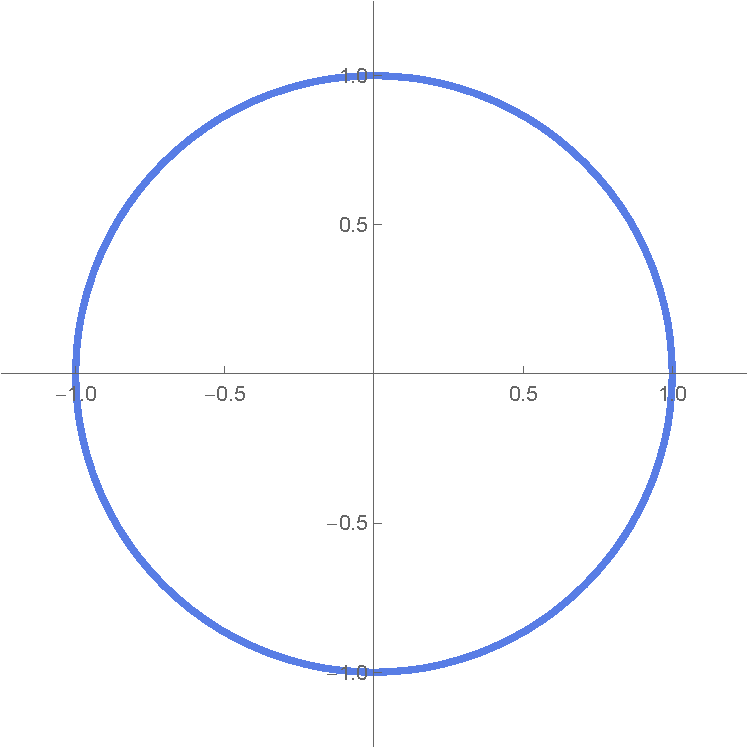
\includegraphics[width=3cm]{fig1.pdf}
  \end{minipage}
  \begin{minipage}{3cm}
    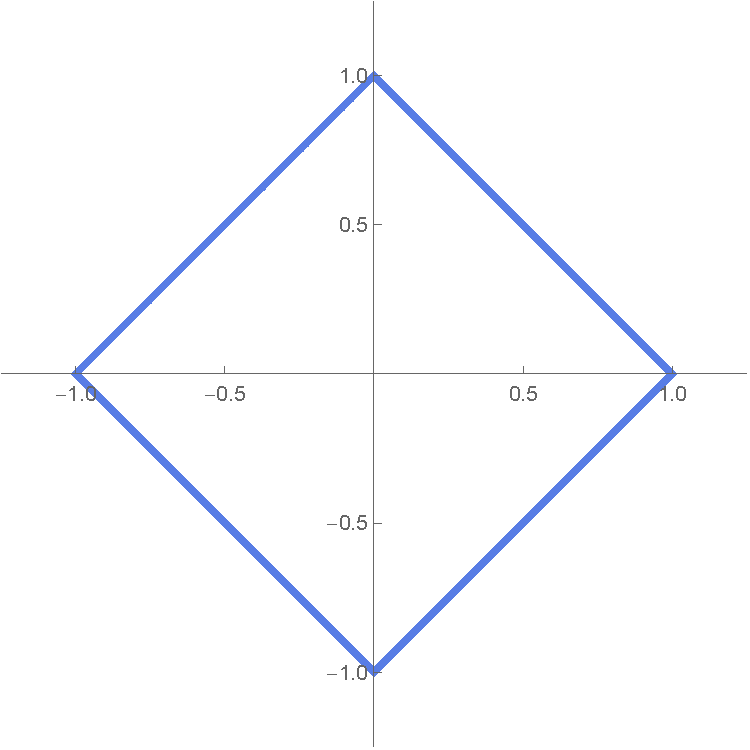
\includegraphics[width=3cm]{fig2.pdf}
  \end{minipage}
  \begin{minipage}{3cm}
    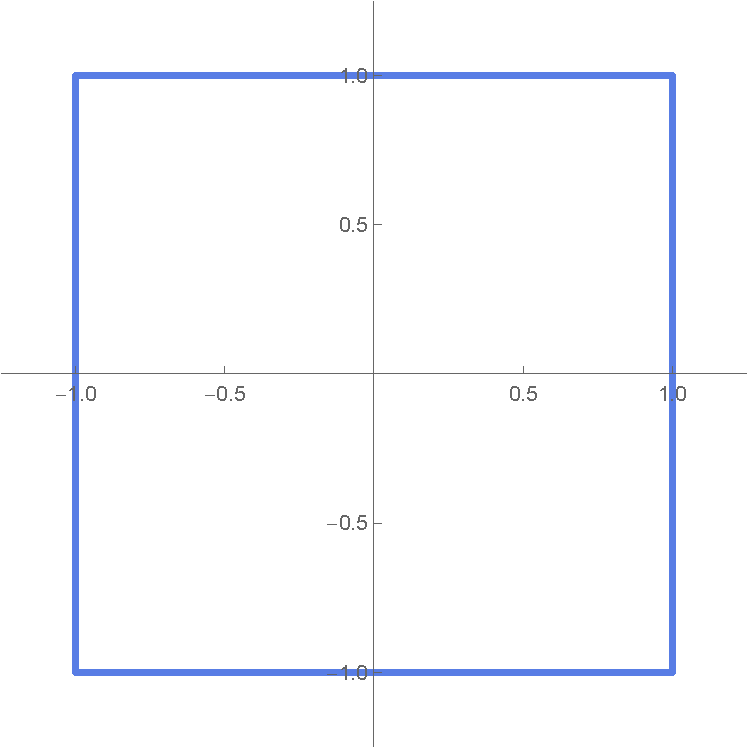
\includegraphics[width=3cm]{fig3.pdf}
  \end{minipage}
  \caption{$\mathbb{R}^2$中球的例子, $\|(x,y)\|_1\leq1, \|(x,y)\|_2\leq1, \|(x,y)\|_3\leq1$}
\end{figure}
\end{example}
\paragraph*{开集和闭集}
\begin{definition}
  $S$是赋范空间$E$的子集, 若对于任意$x\in S$都存在$\varepsilon>0$, 使得$B(x,\varepsilon)\subseteq S$,则称$S$为开集. 如果子集$S$的补集$(E\setminus S)$是开集, 则称$S$为闭集.
\end{definition}
很容易意识到, 尽管球的定义不同, 但范数的等价定义了相同的开集. 开集同样的定义了闭集、稠集和紧集以及其他的拓扑概念.
\begin{example}
  开球是开集. 闭球和球面是闭集.
\end{example}
\begin{theorem}\quad
\begin{enumerate}[(a)]
  \item 开集的任意并集是开集
  \item 开集的有限交集是开集
  \item 闭集的有限并集是闭集
  \item 闭集的任意交集是闭集
  \item 空集和全集既是开也是闭的
\end{enumerate}
\end{theorem}
\begin{theorem}
  赋范空间$E$的子集$S$是闭的, 当且仅当$S$的元素序列在$E$中收敛,并且极限在$S$中.
  \begin{equation*}
    x_1,x_2,\dots,x_n\in S,\quad x_n\to x,\quad x\in S
  \end{equation*}
\end{theorem}
\begin{proof}
  假设$S$是$E$的闭子集, $x_1,x_2,\dots\in S$, $x_n\to x$且$x\notin S$. 因为$S$是闭集, $E\setminus S$是开集. 所以存在$\varepsilon>0$使得$B(x,\varepsilon)\subseteq E\setminus S$. 换句话说,因为$\|x-x_n\|\to 0$, 对于充分大的$n\in \mathbb{N}$, 我们有$\|x-x_n\|<\varepsilon$. 这个矛盾表明了$x\in S$.

  \indent现在假设$x_1,x_2,\dots\in S$, 并且有$x_n\to x$,$x\in S$. 如果$S$不是闭集, 则$E\setminus S$非开. 所以存在$x\in E\setminus S$使得任意球$B(x,\varepsilon)$都包含$S$中的元素. 这样我们能找到$x_1,x_2,\dots\in S$使得$x_n\in B(x,\frac{1}{n})$. 但另一方面$x_n\to x$以及假设条件$x\in S$. 这与$x\in E\setminus S$假设相互矛盾. 因此$S$必须是闭集.
\end{proof}
\paragraph*{闭包}
\begin{definition}
  $S$是赋范空间$E$的子集, $S$的闭包定义为所有闭集的交, 记作$cl S$.表示最小的闭集.
\end{definition}
\begin{theorem}
  $S$是赋范空间$E$的子集, 闭包$cl S$是指$S$中所有收敛列极限的集合.
  \begin{equation*}
    cl S=\{x\in E:\exists x_1,x_2,\dots\in S s.t. x_n\to x\}
  \end{equation*}
\end{theorem}
读者自证
\paragraph*{稠密}
\begin{definition}
  赋范空间$E$有子集$S$, 如果$cl S=E$, 则$S$被称为稠密的,
\end{definition}
\begin{example}
  $[a,b]$上所有多项式的集合在$\mathcal{C}([a,b])$上稠密. 有限项非零项的所有复数列的集合在$l^p(p>1)$上稠密.
\end{example}
\begin{theorem}
  $S$是赋范空间$E$的子集, 以下条件相互等价:
  \begin{enumerate}[(a)]
    \item $S$在$E$中稠密
    \item 对于每一个$x\in E$, 都存在$x_1,x_2,\dots\in S$,使得$x_n\to x$
    \item 对于$E$的每一个非空子集至少包含$S$中的一个元素
  \end{enumerate}
\end{theorem}
\paragraph*{紧致}
\begin{definition}
  赋范空间$E$有子集$S$, 如果$S$中的每一个序列$(x_n)$都包含极限在$S$中的收敛子序列, 则称$S$为紧致集合
\end{definition}
\begin{example}
  $R^n,C^n$中的有界闭集紧致
\end{example}
\begin{theorem}
  当且仅当闭单位球是紧致的时候, 赋范空间$E$是有限维的
\end{theorem}
\paragraph*{有界}
\begin{definition}
  赋范空间$E$中有子集$S$, 如果存在$r>0$, $S\subseteq B(0,r)$, 则称$S$是有界子集
\end{definition}
\begin{theorem}
  紧致集合是有界闭的.
\end{theorem}
\begin{theorem}
  当且仅当$E$中的单位球是紧致的, 赋范空间$E$是有限维的.
\end{theorem}
读者自证
\subsection{Banach空间}
\subsubsection*{Cauchy序列}
\begin{definition}
  如果对于任意$\varepsilon>0$存在数$M$使得$\|x_m-x_n\|<\varepsilon$对于$m,n>M$都成立, 则称赋范空间中的向量序列$(x_n)$为Cauchy序列.
\end{definition}
Augustin Louis Cauchy(1789-1857)
\begin{theorem}
  下列条件相互等价
  \begin{enumerate}[(a)]
    \item $(x_n)$是Cauchy序列.
    \item 对于任意一对递增正整数序列$(p_n),(q_n)$, 都有$\|x_{p_n}-x_{q_n}\|\to0,n\to\infty$成立
    \item 对于任意递增正整数序列$(p_n)$, 都有$\|x_{p_{n+1}}-x_{p_n}\|\to0,n\to\infty$成立
  \end{enumerate}
\end{theorem}
显然每一个收敛序列都是Cauchy序列,事实上若$\|x_n-x\|\to0$, 则
\begin{equation*}
  \|x_{p_n}-x_{q_n}\|\leq\|x_{p_n}-x\|+\|x_{q_n}-x\|\to0
\end{equation*}
对于每一个递增序列$(p_n),(q_n)$都成立.收敛序列是Cauchy序列, 但Cauchy序列不一定是收敛序列.
\begin{example}
  设$\mathcal{P}([0,1])$是$[0,1]$上的多项式空间, 并且有一致收敛的范数$\|P\|=\max_{[0,1]}|P(x)|$. 定义
  \begin{equation*}
    P_n(x)=1+x+\frac{x^2}{2!}+\cdots+\frac{x^n}{n!}
  \end{equation*}
  其中$n=1,2,\dots$, $(P_n)$是一个Cauchy序列, 但显然并不收敛于$\mathcal{P}([0,1])$, 因为极限不是一个多项式.
\end{example}
\begin{lemma}
  若$(x_n)$是赋范空间的一个Cauchy序列, 则序列$(\|x_n\|)$收敛.
\end{lemma}
\begin{proof}
  因为$|\|x\|-\|y\||\leq\|x-y\|$, 所以有$|\|x_m\|-\|x_n\||\leq\|x_m-x_n\|\to0,(m,n\to \infty)$. 范数序列是实柯西序列, 因此它收敛.
\end{proof}
\subsubsection*{Banach空间}
\begin{definition}
  如果每一个Cauchy序列都收敛于$E$,则称$E$是完备的.完备的赋范空间称为Banach空间
\end{definition}
\begin{example}\label{l^2 complete}
  $l^2$是完备空间. 设$(a_n)$是$l^2$的柯西序列, 如果
  \begin{equation*}
    a_n=(\alpha_{n,1},\alpha_{n,2},\dots)
  \end{equation*}
  对于给定的任意$\varepsilon>0$都存在数$n_0$使得
  \begin{equation*}\label{banach l^2}
    \sum_{k=1}^{\infty}|\alpha_{m,k}-\alpha_{n,k}|^2<\varepsilon^2
  \end{equation*}
  对于所有的$m,n\geq n_0$都成立. 值得注意, 这实际上是对于每一个固定的$k\in \mathbb{N}$和每一个$\varepsilon$都存在一个数$n_0$使得
  \begin{equation*}
    |\alpha_{m,k}-\alpha_{n,k}|<\varepsilon
  \end{equation*}
  对于任意$mn,\geq n_0$都成立. 这也意味着对于任意$k$, 序列$(\alpha_{n,k})$是$\mathbb{C}$里的柯西序列, 所以是收敛序列.记
  \begin{equation*}
    \alpha_k=\lim_{n\to\infty}\alpha_{n,k},\quad k=1,2,\dots\quad a=(\alpha_{n})
  \end{equation*}
  进一步证明$a$是$l^2$的元素, 序列$(a_n)$收敛于$a$. 根据\eqref{banach l^2}, 令$m\to \infty$得到
  \begin{equation*}
    \sum_{k=1}^{\infty}|\alpha_k-\alpha_{n,k}|^2\leq\varepsilon^2
  \end{equation*}
  对于任意$n\geq n_0$都成立. 因为
  \begin{equation*}
    \sum_{k=1}^{\infty}|\alpha_{n_0,k}|^2<\infty
  \end{equation*}
  再利用$Minkowski$不等式
  \begin{equation*}
  \begin{split}
     \sqrt{\sum_{k=1}^{\infty}|\alpha_k|^2}&=\sqrt{\sum_{k=1}^{\infty}(|\alpha_k|-|\alpha_{n_0,k}|+|\alpha_{n_0,k}|)^2} \\
       &\leq\sqrt{\sum_{k=1}^{\infty}(|\alpha_k|-|\alpha_{n_0,k}|)^2}+\sqrt{\sum_{k=1}^{\infty}|\alpha_{n_0,k}|^2}\\
       &\leq\sqrt{\sum_{k=1}^{\infty}|\alpha_k-\alpha_{n_0,k}|^2}+\sqrt{\sum_{k=1}^{\infty}|\alpha_{n_0,k}|^2}<\infty
  \end{split}
  \end{equation*}
  这就证明了序列$a=(\alpha_n)$是$l^2$的元素. 因为$\varepsilon$是任意小的, 所以有
  \begin{equation*}
    \lim_{n\to\infty}\|a-a_n\|=\lim_{n\to\infty}\sqrt{\sum_{k=1}^{\infty}(|\alpha_k|-|\alpha_{n,k}|)^2}=0
  \end{equation*}
  序列$(a_n)$收敛于$a$,且$a\in l^2$
\end{example}
\paragraph*{收敛与绝对收敛}
\begin{definition}
  赋范空间$E$中有级数$\sum_{n=1}^{\infty}x_n$, 如果序列的部分和收敛于$E$, 也就是说, 存在$x\in E$使得当$n\to\infty$时$\|x_1+x_2+\cdots+x_n-x\|\to0$成立, 则叫做收敛级数. 这种情况下记作$\sum_{n=1}^{\infty}x_n=x$. 如果$\sum_{n=1}^{\infty}\|x_n\|<\infty$, 则称级数为绝对收敛.
\end{definition}
\begin{theorem}
  Banach空间的闭子空间是Banach空间自己
\end{theorem}
\subsection{线性映射}
我们先介绍一些概念. 设$E_1$和$E_2$是两个向量空间, $L$是$E_1$到$E_2$的映射. 如果$y=L(x)$, 则称$y$是$x$的像.

\indent如果$A$是$E_1$的子集, 则$L(A)$表示$A$的像集, 也就是说, $L(A)$是$A$中元素的像的集合,并且像在$E_2$里. 如果$B$是$E_2$的子集, 则$L^{-1}(B)$表示$B$的原像.
\begin{equation*}
  L(A)={L(x):x\in A},\quad L^{-1}(B)={x\in E_1:L(x)\in B}
\end{equation*}
值得注意的是$L^{-1}$并不意味着$L$是可逆的.

\indent我们通常考虑的映射是定义在向量空间的真子空间上的. 所以提出$L$的定义域这个概念是很重要的, 我们用$\mathcal{D}(L)$表示$L$的定义域. 集合$L(\mathcal{D}(L))$叫做$L$的值域, 用$\mathcal{R}(L)$表示.
\begin{equation*}
  \mathcal{R}(L)=\{y\in E_2:L(x)=y,x\in\mathcal{D}(L)\}
\end{equation*}
$L$的零空间记作$\mathcal{N}(L)$, 这指的是所有的$x\in \mathcal{D}(L)$使得$L(x)=0$. 在最后简单介绍一下映射的图, 用$\mathcal{G}(L)$表示映射$L$的图,指的是如下定义的$E_1\times E_2$的子集
\begin{equation*}
  \mathcal{G}(L)=\{(x,y):x\in\mathcal{D}(L),y=L(x)\}
\end{equation*}
\subsubsection*{线性映射}
\begin{definition}
  如果映射$L:E_1\mapsto E_2$对于任意的$x,y\in E_1,\alpha,\beta\in \mathbf{F}$满足$L(\alpha x+\beta y)=\alpha L(x)+\beta L(y)$, 则称$L$为线性映射
\end{definition}
在向量空间中, 我们常用$Lx$的写法替代$L(x)$.
\subsubsection*{连续映射}
\begin{definition}
  设$E_1$和$E_2$是赋范空间, $F$是$E_1$到$E_2$的映射, 如果对于所有$E_1$中的序列$(x_n)$都收敛于$x_0$, 有序列$(F(x_n))$收敛于$F(x_0)$, 即如果$\|x_n-x_0\|\to0$意味着$\|F(x_n)-F(x_0)\|\to0$, 那么就说$F$在$x_0$连续. 如果$F$在任意$x\in E_1$都连续, 则称$F$是连续的.
\end{definition}
我们将会在量子力学里面遇到很多连续性问题.
\begin{example}
  赋范空间$E$的范数是$E\mapsto\mathbb{R}$的连续映射.
  \begin{proof}
    如果有$\|x_n-x\|\to0$,则$|\|x_n\|-\|x\||\leq\|x_n-x\|\to 0$
  \end{proof}
\end{example}
\begin{theorem}
  设$F:E_1\mapsto E_2$. 下列条件相互等价.
  \begin{enumerate}[(a)]
    \item $F$是连续的
    \item $E_2$的任意开子集$U$的原象$F^{-1}(U)$在$E_1$中仍然是开的.
    \item $E_2$的任意闭子集$S$的原象$F^{-1}(S)$在$E_1$中仍然是闭的.
  \end{enumerate}
\end{theorem}
\begin{theorem}\label{continuous linear map}
  如果存在$x_0\in E_1$, 有线性映射$L:E_1\mapsto E_2$在$x_0$连续, 则线性映射$L$是连续映射的.
\end{theorem}
\begin{proof}
  假设$L$在$x_0\in E_1$连续. 设$x$是$E_1$的任意一个元素$(x_n)$是收敛于$x$的序列. 自然地有序列$(x_n-x+x_0)$收敛于$x_0$,这样我们有$\|Lx_n-Lx\|=\|L(x_n-x+x_0)-Lx_0\|\to 0$. 得证
\end{proof}
\subsubsection*{有界线性映射}
\begin{definition}
  线性映射$L:E_1\mapsto E_2$,如果存在数$\alpha>0$使得对于所有的$x\in E_1$都有$\|Lx\|\leq\|x\|$,则$L$叫做有界线性映射.
\end{definition}
值得注意的是, 这个定义相当于说$L$在$E_1$的单位球面上以$\alpha$为界, 也就是说对于所有的$x\in E_1$有$\|Lx\|\leq\alpha$使得$\|x\|=1$
\begin{theorem}
  线性映射是连续的, 当且仅当它是有界的.
\end{theorem}
\begin{proof}
  如果$L$是有界线性映射,且有$\|x_n\|\to 0$, 则$\|Lx_n\|\leq\alpha\|x_n\|\to 0$. 即线性映射$L$在$0$连续, 根据定理\ref{continuous linear map}, $L$是连续映射.
  \indent如果$L$不是有界的, 那么对于任意$n\in N$, 存在$x_n\in E_1$使得$\|Lx_n\|>n\|x_n\|$.定义序列:
  \begin{equation*}
    y_n=\frac{x_n}{n\|x_n\|}
  \end{equation*}
  显然$y_n\to 0$,而对于任意$n\in N$有$\|Ly_n\|>1$, 所以$L$不是连续映射
\end{proof}
有限维空间的线性映射是有界的,上述定理也意味着对于线性映射连续和一致连续是等价的.

\indent如果加法和数乘如下定义, 向量空间$E_1$到$E_2$的所有线性映射也构成向量空间:
\begin{equation*}
  (L_1+L_2)x=L_1x+L_2x,\quad (\lambda L)x=\lambda(Lx)
\end{equation*}
如果$E_1$和$E_2$是赋范空间, 则所有$E_1\mapsto E_2$的有界线性映射的集合是上面定义的空间的线性子空间, 记作$\mathcal{B}(E_1,E_2)$
\begin{theorem}
  如果$E_1$和$E_2$是赋范空间, 则$\mathcal{B}(E_1,E_2)$也是赋范空间, 范数如下定义:
  \begin{equation*}\label{B norm}
    \|L\|=\sup_{\|x\|=1}\|Lx\|
  \end{equation*}
\end{theorem}
\begin{proof}
  如果$L_1,L_2\in\mathcal{B}(E_1,E_2)$有$x\in E_1$使得$\|x\|=1$, 则有
  \begin{equation*}
    \|L_1x+L_2x\|\leq\|L_1x\|+\|L_2x\|
  \end{equation*}
  这意味着
  \begin{equation*}
    \|L_1x+L_2x\|\leq\sup_{\|x\|=1}\|L_1x\|+\sup_{\|x\|=1}\|L_2x\|=\|L_1\|+\|L_2\|
  \end{equation*}
  因此有,
  \begin{equation*}
    \|L_1+L_2\|=\sup_{\|x\|=1}\|L_1x+L_2x\|\leq\|L_1\|+\|L_2\|
  \end{equation*}
  所以上述范数定义的确满足三角不等式.
\end{proof}
\eqref{B norm}定义的范数是$\mathcal{B}(E_1,E_2)$的标准范数, 当我们谈论起$\mathcal{B}(E_1,E_2)$的范数时, 指的就是这个范数.
\begin{theorem}
  若$E_1$是赋范空间$E_2$是Banach空间, 则$\mathcal{B}(E_1,E_2)$是Banach空间
\end{theorem}
\begin{proof}
  首先说明$\mathcal{B}(E_1,E_2)$是完备的. $(L_n)$是$\mathcal{B}(E_1,E_2)$中的柯西序列, $x$是$E_1$的任意元素.则有:
  \begin{equation*}
    \|L_mx-L_nx\|\leq\|L_m-L_n\|\|x\|\to 0\quad m,n\to\infty
  \end{equation*}
  这表明了$(L_nx)$是$E_2$中的Cauchy序列. 由于$E_2$的完备性, 存在唯一的元素$y\in E_2$使得$L_nx\to y$. 因为$x$是$E_1$的任意元素, 这定义了一个从$E_1$到$E_2$的映射$L$:
  \begin{equation*}
    Lx=\lim_{n\to\infty}L_nx
  \end{equation*}
  接下来再证明$L\in\mathcal{B}(E_1,E_2)$和$\|L_n-L\|\to 0$.
  显然, $L$是一个线性映射. 因为Cauchy序列有界, 存在一个常数$\alpha$使得对于所有的$n\in \mathbb{N}$有$\|L_n\|\leq\alpha$成立. 所以
  \begin{equation*}
    \|Lx\|=\|\lim_{n\to\infty}L_nx\|=\lim_{n\to\infty}\|L_nx\|\leq\alpha\|x\|
  \end{equation*}
  因此$L$也是有界的, 这样$L\in\mathcal{B}(E_1,E_2)$. 接下来还有$\|L_n-L\|\to0$需要证明. 令$\varepsilon>0$, 存在$k$使得对于所有的$m,n\geq k$都有$\|L_m-L_n\|<\varepsilon$. 如果$\|x\|=1,m,n\geq k$,则
  \begin{equation*}
    \|L_mx-L_nx\|\leq\|L_m-L_n\|<\varepsilon
  \end{equation*}
  令$n\to\infty$得到对于任意$m\geq k,x\in E_1,\|x\|=1$有$\|L_mx-Lx\|\leq\varepsilon$. 所以对于所有的$m>k$, $\|L_m-L\|\leq\varepsilon$.得证
\end{proof}
\begin{theorem}
  (对角定理)$E$是一个赋范空间,$(x_{ij}),(i,j\in \mathbb{N})$是$E$中的无限维矩阵的矩阵元. 若有:
  \begin{enumerate}[(a)]
    \item 对于任意$j\in \mathbb{N}$有$\lim_{i\to\infty}x_{ij}=0$
    \item 对于每一个指标列$p_n$有子列$q_n$使得
    \begin{equation*}
      \lim_{i\to\infty}\sum_{j=1}^{\infty}x_{q_jq_j}=0
    \end{equation*}
    则$\lim_{i\to\infty}x_{ii}=0$
  \end{enumerate}
\end{theorem}
留作练习, 读者自证. 下面简单介绍一下压缩映射和不动点定理
\subsubsection*{压缩映射}
\begin{definition}
  赋范空间$E$的子集$A$到$E$之间有一映射$f$, 如果存在正数$\alpha<1$使得对于所有的$x,y\in A$都有:
  \begin{equation*}
    \|f(x)-f(y)\|\leq\alpha\|x-y\|
  \end{equation*}
  则把$f$叫做压缩映射.
\end{definition}
\begin{example}
  考虑一个非线性方程$x^3-x-1=0$. 方程有三个根. 把方程写成$Tx=x$形式有多种方式.例如
  \begin{equation*}
    Tx=(1+x)^{\frac{1}{3}},\quad Tx=x^3-1,\quad Tx=\frac{1}{x^2-1}
  \end{equation*}
  原方程的根在$[1,2]$. 由$T(x)=(1+x)^{\frac{1}{3}}$定义的映射$T$是一个压缩映射. 由均值定理可以得到
  \begin{equation*}
    |Tx-Ty|=|(1+x)^{\frac{1}{3}}-(1+y)^{\frac{1}{3}}|\leq\frac{2^{\frac{1}{3}}}{6}|x-y|
  \end{equation*}
  其余两个不是压缩映射
\end{example}
\subsubsection*{Banach不动点定理}
首先要介绍一下不动点. 如果映射$f$满足存在点$z$使得$f(z)=z$, 则称$z$为$f$的不动点. 这个定理在后面的微分积分方程里有很大的用处.
\begin{example}
  令$E=\mathcal{C}([0,1])$是定义在闭区间$[0,1]$上的连续复函数空间. 再令$T$如下定义
  \begin{equation*}
    (Tx)(t)=x(0)+\int_{0}^{t}x(\tau)d\tau
  \end{equation*}
  显然, 对于任意$a\in \mathbb{C}$, 函数$x(t)=ae^t$是$T$的不动点.
\end{example}
\begin{theorem}
  (不动点定理)令$F$是赋范空间$E$的闭子集, $f$是从$F$到$F$的压缩映射, 则存在唯一的$x\in F$使得$f(z)=z$
\end{theorem}
\begin{proof}
  令$0<\alpha<1$使得对于所有的$x,y\in F$有
  \begin{equation*}
    \|f(x)-f(y)\|\leq\alpha\|x-y\|
  \end{equation*}
  令$x_0$是$F$中的任意点, $x_n=f(x_{n-1}),n=1,2,\dots$. 我们将证明$(x_n)$是Cauchy序列. 首先观察到, 对于任意$n\in \mathbb{N}$
  \begin{equation*}
    \|x_{n+1}-x_n\|\leq\alpha\|x_n-x_{n-1}\|\leq\alpha^2\|x_{n-1}-x_{n-2}\|\leq\cdots\leq\alpha^n\|x_1-x_0\|
  \end{equation*}
  因此对于任意$m,n\in\mathbb{N}$使得$m<n$有
  \begin{equation*}
  \begin{split}
     \|x_n-x_m\| & \leq\|x_n-x_{n-1}\|+\|x_{n-1}-x_{n-2}\|+\cdots+\|x_{m+1}-x_{m}\| \\
       & \leq(\alpha^{n-1}+\alpha^{n-2}+\cdots+\alpha^m)\|x_1-x_0\| \\
       & \frac{\|x_1-x_0\|}{1-\alpha}\alpha^m\to 0,\quad m\to\infty
  \end{split}
  \end{equation*}
  这样$(x_n)$是Cauchy序列. 因为$F$是完备空间的闭子集, 所以存在$z\in F$使得当$n\to\infty$时$x_n\to z$.接下来证明唯一存在$z$使得$f(z)=z$.
  首先因为
  \begin{equation*}\
  \begin{split}
     \|f(z)-z\|&\leq\|f(z)-x_n\|+\|x_n-z\| \\
       &=\|f(z)-f(x_{n-1})\|+\|x_n-z\| \\
       &\leq\alpha\|x-z_{n-1}\|+\|x_n-z\|\to 0,\quad n\to\infty
  \end{split}
  \end{equation*}
  $\|f(z)-z\|=0$, 这样就有$f(z)=z$. 假设有另一个点$w\in F$,$f(w)=w$, 则
  \begin{equation*}
    \|z-w\|=\|f(z)-f(w)\|\leq\alpha\|z-w\|
  \end{equation*}
  因为$0<\alpha<1$,必有$\|z-w\|=0$,这意味着$z=w$
\end{proof}
\subsection{线性空间的同构}
\indent设$a_1,a_2,\cdots,a_n$是线性空间$E$的一组基, 在这组基下, $E$中每一个向量都有确定的坐标, 而向量的坐标可以看成$\mathbf{F}^n$的元素.因此向量与它的坐标之间的对应实质上就是$E$到$\mathbf{F}$的一个映射, 这个映射是单射且满射的. 坐标给出了线性空间$E$与$\mathbf{F}^n$的双射.这个对应最重要体现在运算关系的对应上.

\indent设
\begin{equation*}
\begin{split}
   \mathbf{x}&=x_1a_1+x_2a_2+\cdots+x_na_n=\sum_{i=1}^{n}x_ia_i \\
   \mathbf{y}&=y_1a_1+y_2a_2+\cdots+y_na_n=\sum_{j=1}^{n}y_ja_j
\end{split}
\end{equation*}
即向量$\mathbf{x},\mathbf{y}$的坐标分别是$(x_1,\cdots,x_n),(y_1,\cdots,y_n)$, 那么
\begin{equation*}
\begin{split}
  \mathbf{x}+\mathbf{y}&=(x_1+y_1)a_1+\cdots+(x_n+y_n)a_n\\
  k\mathbf{x}&=kx_1a_1+\cdots+kx_na_n
\end{split}
\end{equation*}
向量$\mathbf{x}+\mathbf{y},k\mathbf{x}$的坐标分别是
\begin{equation*}
\begin{split}
  &(x_1+y_1,x_2+y_2,\cdots,x_n+y_n)=(x_1,\cdots,x_n)+(y_1,\cdots,y_n)\\
  &(kx_1,kx_2,\cdots,kx_n)=k(x_1,x_2,\cdots,x_n)
\end{split}
\end{equation*}
向量的运算可以归结成它们坐标的运算, 因而线性空间$E$的讨论可以归结于$\mathbf{F}^n$的讨论
\begin{definition}
  数域$\mathbf{F}$上两个线性空间$E$与$E'$称为同构的, 如果从$E$到$E'$有一个双射$\sigma$. 具有以下性质:
  \begin{enumerate}[(1)]
    \item $\sigma(a+b)=\sigma(a)+\sigma(b)$
    \item $\sigma(ka)=k\sigma(a)$
  \end{enumerate}
  \indent其中$a,b$是$E$中任意向量, k是$\mathbb{F}$中任意数, 这样的映射称为同构映射.
\end{definition}
\indent同构映射基本性质:
\begin{enumerate}[(1)]
  \item $\sigma(0)=0,\sigma(-a)=-\sigma(a)$
  \item $\sigma(\sum_{i=1}^{n}k_ia_i)=\sum_{i=1}^{n}k_i\sigma(a_i)$
  \item $E$中向量组$a_1,\cdots,a_n$线性相关的充分必要条件是, 它们的像$\sigma(a_1),\sigma(a_2),\cdots,\sigma(a_n)$线性相关
  \item 如果$E_1$是$E$的一个线性子空间,那么, $E_1$在$\sigma$下像集合
  \begin{equation*}
    \sigma(E_1)={\sigma(a)|a\in E_1}
  \end{equation*}
  是$\sigma(E)$的子空间, 并且$dim(E_1)=dim(\sigma(E_1))$
  \item 同构映射的逆以及两个同构映射的乘积还是同构映射
\end{enumerate}
\subsection{线性变换}
\subsubsection*{线性变换基本概念}
\indent线性空间中,事物之间的联系反映为线性空间的映射,线性空间到自身的映射通常称为$E$的一个变换.线性变换是最简单最基本的一种变换,线性变换是量子力学里最常用的概念.
\begin{definition}
  如果对于线性空间$E$中任意元素$a,b$和数域$\mathbf{F}$中任意数$k$, 都有这样的线性变换$A$, 满足:
  \begin{equation*}
  \begin{split}
     A(a+b)=A(a)+A(b)\\
     &A(ka)=kA(a)
  \end{split}
  \end{equation*}
  则这个变换$A$称为线性变换, 以后使用大写$A,B,\cdots$代表$E$的变换,$A(a)$或$Aa$代表元素$a$在变换$A$下的像.\textbf{线性变换保持加法与数量乘法}.
\end{definition}
\begin{example}
  平面上的向量构成实数域上的二维线性空间.把平面围绕坐标原点绕逆时针方向转动$\theta$角, 就是一个线性变换, 用$A_\theta$表示.如果平面上一个向量$a$在直角坐标系下的坐标是$(x,y)$, 那么像$A_\theta(a)$的坐标(x',y')为:
  \begin{equation*}
    \begin{pmatrix}
      x' \\
      y' \\
    \end{pmatrix}=\begin{pmatrix}
                    cos\theta & -sin\theta \\
                    sin\theta & cos\theta \\
                  \end{pmatrix}\begin{pmatrix}
                                 x \\
                                 y \\
                               \end{pmatrix}
  \end{equation*}
  \indent同样的三维空间中绕轴有限转动也是一个线性变换
\end{example}
\begin{example}
  线性空间$E$中的恒等变换(单位变换)满足:
  \begin{equation*}
    I(a)=a\quad(a\in E)
  \end{equation*}
  以及零变换$0$:$0(a)=0\quad (a\in E)$
\end{example}
\subsubsection*{线性变换的运算}
线性变换作为映射, 利用映射的复合可以定义线性变换的乘法
\begin{definition}
  设$A,B$是线性空间$E$上的两个线性变换,定义他们乘积$AB$为
  \begin{equation*}
    (AB)(a)=A(B(a))\quad (a\in E)
  \end{equation*}
  容易得到, 线性变换的乘积也是线性变换(读者自证)
\end{definition}
通过以上定义可以看出线性变换满足乘法结合律
\begin{equation*}
  (AB)C=A(BC)
\end{equation*}
但线性变换的乘法一般是不可交换的.
\begin{example}
  实数域$R$上的线性空间$R[x]$中, 线性变换
  \begin{equation*}
    \begin{split}
       D(f(x))&=f'(x)\\
       F(f(x))&=\int_{0}^{x}f(t)dt
    \end{split}
  \end{equation*}
  的乘积$DF=I$,但一般$FD\neq I$
\end{example}
线性变换还可以定义加法.设$A,B$是线性空间$E$上的两个线性变换, 定义它们的和$A+B$为
\begin{equation*}
  (A+B)(a)=A(a)+B(a)\quad a\in E
\end{equation*}
线性变换的和还是线性变换, 不难证明线性变换的加法满足加法结合律与交换律. 对于加法, 零变换$0$有特殊地位, 它与所有线性变换$A$的和仍为$A$:
\begin{equation*}
  A+0=A
\end{equation*}
同样可以定义负变换
\begin{equation*}
  (-A)(a)=-A(a)\quad a\in E
\end{equation*}
显然:$A+(-A)=0$.

\subsection{Hilbert空间}\label{Hilbert Space}
在复习Hilbert空间之前,我们先复习对偶空间的概念.设$E$是实数域$\mathbb{R}$上的$n$维向量空间, 可定义$E$上的线性映射$L$. 即向量空间$E$与实数域$\mathbb{R}$间的线性映射
\begin{equation*}
\begin{split}
   L&:R\mapsto R \\
     x\mapsto&L(x)\in \mathbb{R},\quad x\in E
\end{split}
\end{equation*}
线性映射保持线性结构.
\begin{equation*}
  L(\alpha x+\beta y)=\alpha L(x)+\beta L(y),\quad x,y\in E,\alpha,\beta\in\mathbb{R}
\end{equation*}
在之前的线性映射章节里, 我们讨论了$E_1\mapsto E_2$的线性映射的集合也构成向量空间$\mathcal{B}(E_1,E_2)$.这里我们把这个向量空间$\mathcal{B}(E,\mathbb{R})$称为向量空间$E$的对偶空间, 记作$E^*$
\begin{equation*}
  L\in E^*=\mathcal{B}(E,\mathbb{R})
\end{equation*}
如果$(e_1,e_2,\dots,e_n)$为向量空间的$E$一组基底, 任意向量$x$可用这组基展开
\begin{equation*}
  x=x_1e_1+x_2e_2+\cdots+x_ne_n, \quad x_i\in\mathbb{R},n=1,2,\dots
\end{equation*}
由于线性映射保证线性结构不变.
\begin{equation*}
  Lx=x_1Le_1+x_2Le_2+\cdots+x_nLe_n, \quad x_i\in\mathbb{R},n=1,2,\dots
\end{equation*}
即所有的线性映射$L$都可以由它们在基底$e_i$上取的值决定.记
\begin{equation*}
  L_i=Le_i\in\mathbb{R}
\end{equation*}
称为对偶向量$L$的分量, 可将$L\in E^*$记作
\begin{equation*}
  f=f_1e_1^*+f_2e_2^*+\cdots f_ne_n^*
\end{equation*}
其中$e_i^*\in E^*$, 为向量空间中满足下列条件的线性映射.
\begin{equation*}
  e_i^*(e_k)=\delta_{ik}
\end{equation*}
显然这组线性映射$e_1^,e_2^*,\dots,e_n^*$线性无关. 它们形成了$E^*$中的一组基, 称为与基$(e_1,e_2,\dots,e_n)$对偶的基. 对偶空间$E^*$也为$n$维向量空间, 且空间$E$与空间$E^*$相互对偶.

\indent向量空间$E$和$E$上的线性映射空间$E^*$是两个重要概念, 为帮助熟悉他的含义, 我们采用熟悉的Dirac符号去表示.向量空间$E$上的元素$x$可以用$|x\rangle$去表示. 基组$(e_1,e_2,\dots,e_n)$可以用$(|1\rangle,|2\rangle,\dots,|n\rangle)$去表示.
\begin{equation*}
  |x\rangle=x_1|1\rangle+x_2|2\rangle+\cdots+x_n|n\rangle
\end{equation*}
对偶空间$E^*$上的元素$L$记作$\langle L|$, 基组$(e_1^*,e_2^*,\dots,e_n^*)$记作$(\langle1|,\langle2|,\dots,\langle n|)$
\begin{equation*}
  \langle L|=L_1\langle1|+L_2\langle2|+\cdots+L_n\langle n|
\end{equation*}
基矢$\langle i|,i=1,\dots,n$由它对整个向量空间$E$的作用决定
\begin{equation*}
  \langle i|j\rangle=\delta_{ij}
\end{equation*}
值得注意, $E$与$E^*$均为线性空间, 在$E$与$E^*$之间可以定义内积
\begin{equation*}
  \langle L|x\rangle=\sum_{k=1}^{k=n}L_kx_k
\end{equation*}
\subsubsection*{内积空间}
我们现在开始讨论定义了内积的复向量空间, 内积的定义如下. 这里$\mathbf{F}=\mathbb{C}$, 对于$x\in\mathbb{C}$, 复共轭的标记我们用$x^*$表示.
\begin{definition}\label{inner def}
  令$E$是一个复向量空间, 有映射$\langle\cdot,\cdot\rangle\mapsto\mathbb{C}$, 如果对于任意$x,y,z\in E$和$\alpha,\beta\in \mathbb{C}$满足下列条件
  \begin{enumerate}[(a)]
    \item\label{inner a} $\langle x,y\rangle=\langle y,x\rangle^*$
    \item\label{inner b} $\langle x,\alpha y+\beta z\rangle=\alpha\langle x,z\rangle+\beta\langle y,z\rangle$
    \item $\langle x,x\rangle\geq 0$
    \item $\langle x,x\rangle=0$当且仅当$x=0$
  \end{enumerate}
  则把这个映射叫做内积.具有内积的向量空间叫做向量空间
\end{definition}
根据定义, 两个向量的内积是复数. 根据条件\ref{inner a}, $\langle x,x\rangle=\langle x,x\rangle^*$, 对于任意$x\in E$, $\langle x,x\rangle$是实数. 根据\ref{inner b}可以得到关系式
\begin{equation*}
  \langle\alpha x+\beta y,z\rangle=\langle z,\alpha x+\beta y\rangle^*=(\alpha\langle z,x\rangle+\beta\langle z,y\rangle)^*=\alpha^*\langle z,x\rangle^*+\beta^*\langle z,y\rangle^*=\alpha^*\langle x,z\rangle+\beta^*\langle y,z\rangle
\end{equation*}
特别的
\begin{equation*}
  \langle\alpha x,y\rangle=\alpha^*\langle x,y\rangle,\quad \langle x,\alpha y\rangle=\alpha\langle x,y\rangle
\end{equation*}
因此如果$\alpha=0$我们有$\langle 0,y\rangle=\langle x,0\rangle=0$
\begin{example}
  最简单最重要的内积空间例子是复数空间$\mathbb{C}$. 其中内积的定义是$\langle x,y\rangle=x^*y$
\end{example}
\begin{example}
  $n$元复数数组$x=(x_1,\dots,x_n)$的空间$\mathbb{C}^n$, 构成内积空间, 其内积的定义是
  \begin{equation*}
    \langle x,y\rangle=\sum_{k=1}^{n}x_k^* y_k,\quad x=(x_1,\dots,x_n),y=(y_1,\dots,y_n)
  \end{equation*}
\end{example}
\begin{example}\label{l^2 inner space}
  所有复数序列$(x_1,x_2,x_3,\dots)$构成的$l^2$空间$(\sum_{k=1}^{\infty}|x_k|^2<\infty)$是一个内积空间, 其内积定义是
  \begin{equation*}
    \langle x,y\rangle=\sum_{k=1}^{\infty}x_k^*y_k,\quad x=(x_1,x_2,x_3,\dots),y=(y_1,y_2,y_3\dots)
  \end{equation*}
  之后我们将会见到, 这个空间是内积空间里最重要的例子.
\end{example}
\begin{example}\label{nonzero term}
  仅有限非零项的复数序列$(x_1,x_2,x_3,\dots)$构成的空间是一个内积空间, 内积的定义如\ref{l^2 inner space}.
\end{example}
\begin{example}\label{C[a,b]inner}
  区间$[a,b]$上的连续复函数的空间$\mathcal{C}([a,b])$是一个内积空间, 内积定义如下
  \begin{equation*}
    \langle f,g\rangle=\int_{a}^{b}f^*(x)g(x)dx
  \end{equation*}
\end{example}
\begin{example}
  $L^2(\mathbb{R})$是内积空间, 内积定义如下:
  \begin{equation*}
    \int_{-\infty}^{+\infty}f^*(x)g(x)dx
  \end{equation*}
  进一步说, $L^2(\mathbb{R}^n)$也是内积空间, 其内积定义是
  \begin{equation*}
    \int_{\mathbb{R}^n}f^*(x)g(x)dx
  \end{equation*}
\end{example}
\begin{example}
  令$E$是内积空间$E_1$和$E_2$的Cartesian乘积, $E=E_1\times E_2={(x,y):x\in E_1,y\in E_2}$. 空间$E$是一个内积空间, 其内积定义如下:
  \begin{equation*}
    \langle(x_1,y_1),(x_2,y_2)\rangle=\langle x_1,x_2\rangle+\langle y_1,y_2\rangle
  \end{equation*}
  值得注意$E_1$和$E_2$可以分别的看成子空间$E\times{0}$和${0}\times E_2$
\end{example}
内积空间是具有内积的向量空间, 每一个内积空间也是赋范空间, 范数如下定义
\begin{equation*}
  \|x\|=\sqrt{\langle x,x\rangle}
\end{equation*}
首先注意函数是良定义的, 因为$\langle x,x\rangle$总是非负的实数, 并且$\|x\|=0$当且仅当$x=0$. 进一步说
\begin{equation*}
  \|\lambda x\|=\sqrt{\langle\lambda x,\lambda x\rangle}=\sqrt{\lambda^*\lambda\langle x,x\rangle}=|\lambda|\|x\|.
\end{equation*}
还剩下三角不等式有待证明, 这不像前两个条件这样好证明. 首先我们介绍一下Cauchy-Schwarz不等式.
\begin{theorem}
  对于内积空间里的任意两个元素$x,y$, 有
  \begin{equation}\label{Cauchy-Schwarz}
    |\langle x,y\rangle|\leq\|x\|\|y\|
  \end{equation}
  当且仅当$x,y$线性相关时, 等式$|\langle x,y\rangle|=\|x\|\|y\|$成立.
\end{theorem}
\begin{proof}
  若$y=0$, 则\eqref{Cauchy-Schwarz}刚好满足, 左右两边均是$0$. 假设$y\neq 0$, 我们有
  \begin{equation*}\label{Cauchy-Schwarz proof1}
    0\leq\langle x+\alpha y,x+_\alpha y\rangle=\langle x,x\rangle+\alpha\langle x,y\rangle+\alpha^*\langle y,x\rangle+|\alpha|^2\langle y,y\rangle
  \end{equation*}
  在\eqref{Cauchy-Schwarz proof1}中令$\alpha=-\frac{\langle y,x\rangle}{\langle y,y\rangle}$. 两边同时乘以$\langle y,y\rangle$.
  \begin{equation*}
    0\leq\langle x,x\rangle\langle y,y\rangle-|\langle x,y\rangle|^2
  \end{equation*}
  这就给出了Cauchy-Schwarz不等式. 如果$x,y$线性相关, 存在$\alpha\in \mathbb{C}$有$x=\alpha y$. 因此
  \begin{equation*}
    |\langle x,y\rangle|=|\langle x,\alpha x\rangle|=|\alpha|\langle x,x\rangle=|\alpha|\|x\|\|x\|=\|x\|\|\alpha x\|=\|x\|\|\alpha y\|
  \end{equation*}
  令$x,y$是两个向量,使得$|\langle x,y\rangle|=\|x\|\|y\|$, 也就是说
  \begin{equation*}
    \langle x,y\rangle\langle y,x\rangle=\langle x,x\rangle\langle y,y\rangle
  \end{equation*}
  接下来利用Cauchy-Schwarz不等式等号成立条件去证明$\langle y,y\rangle x-\langle y,x\rangle y=0$, 这表明了$x,y$线性相关.
  \begin{equation*}
  \begin{split}
     \langle\langle y&,y\rangle x-\langle y,x\rangle y,\langle y,y\rangle x-\langle y,x\rangle y\rangle \\
       & =|\langle y,y\rangle|^2\langle x,x\rangle-\langle y,y\rangle\langle y,x\rangle\langle x,y\rangle-\langle y,x\rangle\langle y,y\rangle\langle y,x\rangle+|\langle x,y\rangle|\langle y,x\rangle\langle y,y\rangle \\
       & =0
  \end{split}
  \end{equation*}
  证毕.
\end{proof}
\begin{corollary}
  (三角不等式)对于内积空间中的任意两个元素$x,y$有:
  \begin{equation*}
    \|x+y\|\leq\|x\|+\|y\|
  \end{equation*}
\end{corollary}
\begin{proof}
  \begin{equation*}
  \begin{split}
     \|x+y\|^2& =\langle x+y,x+y\rangle=\langle x,x\rangle+2Re\langle x,y\rangle+\langle y,y\rangle \\
       & \leq\langle x,x\rangle+2|\langle x,y\rangle|+\langle y,y\rangle \\
       & \leq\|x\|^2+2\|x\|\|y\|+\|y\|^2 \\
       & (\|x\|+\|y\|)^2
  \end{split}
  \end{equation*}
  其中$Re z$表示$z\in \mathbb{C}$的实部.
\end{proof}
\paragraph*{内积空间的范数}
\begin{definition}
  根据$\|x\|=\sqrt{\langle x,x\rangle}$可以定义内积空间$E$的范数.
\end{definition}
我们已经证明了每一个内积空间都是赋范空间. 很自然的我们会问到, 是否每一个赋范空间是内积空间呢? 更精确地表述是:是否可能在赋范空间$(E,\cdot)$中定义一个内积$\langle\cdot,\cdot\rangle$使得对于每一个$x\in E$, 有 $\|x\|=\sqrt{\langle x,x\rangle}$? 一般来说, 答案是否定的. 接下来我们将会给出内积空间范数的性质, 这些性质对于赋范空间称为内积空间是充分必要的.
\begin{theorem}
  (平行四边形法则)对于内积空间中任意两个元素, 有:
  \begin{equation*}
    \|x+y\|^2+\|x-y\|^2=2(\|x\|^2+\|y\|^2)
  \end{equation*}
\end{theorem}
\begin{proof}
  我们有
  \begin{equation*}
    \|x+y\|^2=\langle x+y,x+y\rangle=\langle x,x\rangle+\langle x,y\rangle+\langle y,x\rangle+\langle y,y\rangle
  \end{equation*}
  因此
  \begin{equation*}
    \|x+y\|^2=\|x\|^2+\langle x,y\rangle+\langle y,x\rangle+\|y\|^2
  \end{equation*}
  现在令$y\to -y$, 上式得到
  \begin{equation*}
    \|x-y\|^2=\|x\|^2-\langle x,y\rangle-\langle y,x\rangle+\|y\|^2
  \end{equation*}
  两式叠加可得平行四边形法则
\end{proof}
内积空间里最重要的是可以定义正交向量.这使得Hilbert空间与Banach空间非常的不同.
\begin{definition}
  (正交向量)内积空间里有两个向量$x,y$, 如果$\langle x,y\rangle=0$, 则称这两个向量正交,记作$x\perp y$
\end{definition}
如果$x\perp y$, 则有$\langle y,x\rangle=\langle x,y\rangle^*=0$, 因此$y\perp x$. 换句话说, $\perp$关系式对称的.
\begin{theorem}
  (勾股定理)对于任意一对正交向量$x,y$, 我们有
  \begin{equation*}
    \|x+y\|^2=\|x\|^2+\|y\|^2
  \end{equation*}
\end{theorem}
\begin{proof}
  如果$x\perp y$, 则$\langle x,y\rangle=0$, 根据平行四边形法则, 立即可以得到上式.
\end{proof}
在之前我们定义的内积空间都是在$\mathbb{C}$中定义的. 我们也可以在$\mathbb{R}$上定义内积空间, 也就是说任意两个向量的内积是一个实数. 内积的定义\ref{inner def}中的\ref{inner b}要修改成$\langle x,y\rangle=\langle y,x\rangle$, 而之前所有的定理和例子都要修改成$\mathbb{R}$上成立. 有限维实内积空间也叫做Euclidean空间

\indent如果$R^n$上有$x=(x_1,x_2,\dots),y=(y_1,y_2,\dots)$, 则内积的定义$\langle x,y\rangle=\sum_{k=1}^{n}x_ky_k$等价于定义$\langle x,y\rangle=\|x\|\|y\|cos\theta$, 其中$\theta$是向量$x,y$的夹角. 在这种情况下, Cauchy-Schwarz不等式成为
\begin{equation*}
  \frac{|\langle x,y\rangle|}{\|x\|\|y\|}=cos\theta\leq 1,\quad x\neq0,y\neq0
\end{equation*}
\subsubsection*{希尔伯特空间}
\begin{definition}
  完备内积空间叫做Hilbert空间
\end{definition}
这里$E$的完备性是指用$E$的内积定义的范数的完备性.我们现在给出一些内积空间和Hilbert空间的例子
\begin{example}
  由于$\mathbb{C}$与$\mathbb{C}^n$是完备的, 它们都是Hilbert空间.
\end{example}
\begin{example}
  $l^2$是Hilbert空间, 其完备性在之前例子\ref{l^2 complete}已经证明过了, 这里不再复述.
\end{example}
\begin{example}
  例子\ref{nonzero term}里的空间$E$不是Hilbert空间, 考虑柯西序列序列
  \begin{equation*}
    x_n=(1,\frac{1}{2},\frac{1}{3},\dots,\frac{1}{n},0,0,\dots)
  \end{equation*}
  序列满足
  \begin{equation*}
    \lim_{m,n\to\infty}\|x_m-x_m\|=\lim_{n,m\to\infty}\left[\sum_{k=\min{\{m,n\}+1}}^{\max\{m,n\}}\frac{1}{k^2}\right]^{\frac{1}{2}}=0
  \end{equation*}
  然而这个序列并不收敛于$E$中. 因为极限$(1,\frac{1}{2},\frac{1}{3},\dots)$不在$E$中.
\end{example}
\begin{example}
  例子\ref{C[a,b]inner}中的空间是另一个不完备的内积空间例子. 事实上,考虑$\mathcal{C}([0,1])$中的如下函数序列:
  \begin{equation*}
    f_n{x}=\begin{cases}
             1  & \text{如果$0\leq x\leq\frac{1}{2}$} \\
             1-2n\left(x-\frac{1}{2}\right)  & \text{如果$\frac{1}{2}\leq x\leq \frac{1}{2n}+\frac{1}{2}$} \\
             0  & \text{如果$\frac{1}{2n}+\frac{1}{2}\leq x\leq 1$}
           \end{cases}
  \end{equation*}
  显然$f_n$是连续的. 进一步可知
  \begin{equation*}
    \|f_n-f_m\|\leq\left(\frac{1}{n}+\frac{1}{m}\right)^\frac{1}{2}\to 0,\quad\text{当$m,n\to\infty$}
  \end{equation*}
  因此$(f_n)$是柯西序列. 显然这个序列是逐点收敛于函数
  \begin{equation*}
    f(x)=\begin{cases}
           1 & \text{如果$0\leq x\leq \frac{1}{2}$}\\
           0 & \text{如果$\frac{1}{2}\leq x\leq 1$}
         \end{cases}
  \end{equation*}
  函数极限不连续, 因此它不属于$\mathcal{C}([0,1])$, 序列$(f_n)$不收敛于$\mathcal{C}([0,1])$. $\mathcal{C}([0,1])$不是Hilbert空间.
\end{example}
\begin{example}
  $L^2(R)$和$L^2([a,b])$是Hilbert空间
\end{example}
\begin{example}
  $\rho$是区间$[a,b]$上的可测函数且在$[a,b]$上$\rho(x)>0$.记$L^{2,\rho}([a,b])$为$[a,b]$上复可测函数构成的空间
  \begin{equation*}
    \int_{a}^{b}|f(x)|^2\rho(x)dx<\infty
  \end{equation*}
  这是定义了内积
  \begin{equation*}
    \langle f,g\rangle=\int_{a}^{b}f^*(x)g(x)\rho(x)dx
  \end{equation*}
  的一个Hilbert空间. 为了证明完备性, 考虑$L^{2,\rho}([a,b])$上的柯西序列$(f_n)$.
  \begin{equation*}
    \|f_m-f_n\|^2_{L^{2,\rho}([a,b])}=\int_{a}^{b}|f_m(x)-f_n(x)|^2\rho(x)dx\to 0\quad\text{当$n\to\infty$}
  \end{equation*}
  定义
  \begin{equation*}
    F_n=f_n\sqrt{\rho},\quad n\in\mathbb{N}
  \end{equation*}
  因为
  \begin{equation*}\
  \begin{split}
     \|F_m-F_n\|^2_{L^2{([a,b])}} & =\int_{a}^{b}|F_m(x)-F_n(x)|^2dx \\
       & =\int_{a}^{b}|f_m(x)\sqrt{\rho(x)}-f_n(x)\sqrt{\rho(x)}|^2dx\\
       & =\int_{a}^{b}|f_m(x)-f_n(x)|^2\rho(x)dx \\
       & =\|f_m-f_n\|^2_{L^{2,\rho}([a,b])}
  \end{split}
  \end{equation*}
  $(F_n)$是$L^2([a,b])$中的柯西序列.因此存在$F\in L^2([a,b])$使得
  \begin{equation*}
    \|F_n-F_m\|^2_{L^2([a,b])}=\int_{a}^{b}|F_n(x)-F(x)|^2dx\to 0
  \end{equation*}
  我们很容易看到$f_n\to\frac{F}{\sqrt{\rho}} \in L^{2,\rho}([a,b])$, 证明完毕
\end{example}
\begin{example}
  (Sobolev空间)$\Omega$是$\mathbb{R}^n$的一个开集. 所有复函数$f\in\mathcal{C}^m(\Omega)$构成的空间记作$\tilde{H}^m(\Omega),m=1,2,\dots$, 使得对于所有的$|\alpha|\leq m$有$D^\alpha f\in L^2(\Omega)$成立, 其中$\alpha=(\alpha_1,\dots,\alpha_n), \alpha_1,\dots,\alpha_n$是非负整数, $|\alpha|=\alpha_1+\cdots+\alpha_n$, 以及
  \begin{equation*}
    D^\alpha f=\frac{\partial^{|\alpha|f}}{\partial x_1^{\alpha_1}\partial x_2^{\alpha_2}\dots\partial x_n^{\alpha_n}}
  \end{equation*}
  例如, 如果$n=2,\alpha=(2,1)$, 我们有
  \begin{equation*}
    D^\alpha f=\frac{\partial^3 f}{\partial x_1^2\partial x_2}
  \end{equation*}
  对于$f\in\tilde{H}^m(\Omega)$, 对于每一个多元指标$\alpha=(\alpha_1,\alpha_2,\dots,\alpha_n)$, 我们有
  \begin{equation*}
    \int_{\Omega}|\frac{\partial^{|\alpha| f}}{\partial x_1^{\alpha_1}\partial x_2^{\alpha_2}\dots\partial x_n^{\alpha_n}}|^2<\infty
  \end{equation*}
  使得$|\alpha|\leq m$. $\tilde{H}^m(\Omega)$中的内积如下定义:
  \begin{equation*}
    \langle f,g\rangle=\int_{\Omega}\sum_{|\alpha|\leq m}(D^\alpha f)^*D^\alpha g
  \end{equation*}
  如果$\Omega\in \mathbb{R}^2$, $\tilde{H}^2(\Omega)$的内积就是
  \begin{equation*}
    \langle f,g\rangle=\int_{\Omega}(f^*g+f_x^*g_x+f_y^*g_y+f_{xx}^*g_{xx}+f_{yy}^*g_{yy}+f_{xy}^*g_{xy})
  \end{equation*}
  如果$\Omega=(a,b)\subset \mathbb{R}$, $\tilde{H}^m(a,b)$的内积就是
  \begin{equation*}
    \langle f,g\rangle=\int_{a}^{b}\sum_{n=0}^{m}(\frac{d^n f}{dx^n})^* \frac{d^n g}{dx^n}
  \end{equation*}
  $\tilde{H}^m(\Omega)$是一个内积空间, 但不是Hilbert空间, 因为它不完备. 完备的$\tilde{H}^m(\Omega)$记作$H^m(\Omega)$, 它是希尔伯特空间. $H^m(\Omega)$是更一般空间$W^{m,p}(\Omega)$(Sobolev空间)的特殊情况. 我们有$H^m(\Omega)=W^{m,2}(\Omega)$. 由于偏微分方程的广泛应用, $H^m(\Omega)$是最重要的一个Hilbert空间.
\end{example}
因为每一个内积空间都有范数, 所以它也有由范数定义的收敛. 这个收敛叫做强收敛
\paragraph*{强收敛}
\begin{definition}
  内积空间$E$中的序列$(x_n)$, 如果当$n\to\infty$时有$\|x_n-x\|\to 0$, 则称序列$(x_n)$强收敛于$E$中的向量$x$.
\end{definition}
强收敛这个词是为了区别于弱收敛.
\paragraph*{弱收敛}
\begin{definition}
  内积空间$E$中有序列$(x_n)$, 如果当$n\to \infty$时对于任意$y\in E$有$\langle x_n,y\rangle\to\langle x,y\rangle$, 则称序列$(x_n)$弱收敛于$E$中的向量$x$
\end{definition}
上述定义可以写成当$n\to\infty$时, 对于任意$y\in E$有$\langle x_n-x,y\rangle\to 0$. 我们通常用$x_n\to x$表示强收敛, $x_n\stackrel{w}{\to} x$表示弱收敛
\begin{theorem}
  强收敛必定弱收敛, 也就是说, $x_n\to x$意味着$x_n\stackrel{w}{\to}x$
\end{theorem}
\begin{proof}
  设序列$(x_n)$强收敛于$x$. 也就是说当$n\to \infty$时, 有$\|x_n-x\|\to 0$. 根据Cauchy-Schwarz不等式
  \begin{equation*}
    |\langle x_n-x,y\rangle|\leq\|x_n-x\|\|y\|\to 0\text{当$n\to\infty$}
  \end{equation*}
  这样, 当$n\to \infty$时, 对于任意$y\in E$, 有$\langle x_n-x,y\rangle\to 0$.
\end{proof}
对于内积空间$E$中任意的固定点$y$, 映射$\langle\cdot,y\rangle:E\mapsto\mathbb{C}$是$E$上的一个线性泛函. 上述定理告诉了我们对于任意$y\in E$, 这个线性泛函连续. 同样的线性泛函$\langle x,\cdot\rangle\mapsto\mathbb{C}$也连续.
\begin{theorem}
  如果$x_n\to x,y_n\to y$, 则$\langle x_n,y_n\rangle\to\langle x,y\rangle$
\end{theorem}
\begin{proof}
  若$x_n\to x,y_n\to y$, 则有
  \begin{equation*}
  \begin{split}
     |\langle x_n,y_n\rangle-\langle x,y\rangle|& \leq|\langle x_n,y_n\rangle-\langle x,y_n\rangle|+|\langle x,y_n\rangle-\langle x,y\rangle| \\
       & =|\langle x_n-x,y_n\rangle|+|\langle x,y_n-y\rangle| \\
       & \leq\|x_n-x\|\|y_n\|+\|x\|\|y_n-y\|\to 0
  \end{split}
  \end{equation*}
  其中序列$(y_n)$有界.
\end{proof}
根据这个定理, 我们立马可以获得强收敛的一个性质:
\begin{equation*}
  x_n\to x\text{意味着$\|x_n\|\to\|x\|$}
\end{equation*}
\begin{theorem}
  若$x_n\stackrel{w}{\to}x$且$\|x_n\|\to\|x\|$, 则$x_n\to x$.
\end{theorem}
\begin{proof}
  若对于所有的$y$,有$x_n\stackrel{w}{\to}x$, 我们有:
  \begin{equation*}
    \langle x_n,x\rangle\to\langle x,y\rangle,\quad n\to\infty
  \end{equation*}
  因此
  \begin{equation*}
    \langle x_n,x\rangle\to\langle x,x\rangle=\|x\|^2
  \end{equation*}
  现在, 当$n\to\infty$时
  \begin{equation*}
    \begin{split}
       \|x_n-x\|^2 & =\langle x_n-x,x_n-x\rangle \\
         & =\langle x_n,x_n\rangle-\langle x_n,x\rangle-\langle x,x_n\rangle+\langle x,x\rangle \\
         & =\|x_n\|^2-2Re\langle x_n,x\rangle+\|x\|^2\to\|x\|^2-2\|x\|^2+\|x\|^2=0
    \end{split}
  \end{equation*}
  因此序列$(x_n)$强收敛于$x$
\end{proof}
\subsection{正交归一系统}
向量空间中可以给定一族基$\mathcal{B}$, 使得任意向量$x\in E$能被写成$\sum_{n=1}^{m}\lambda_nx_n$, 其中$x_n\in \mathcal{B}$, $\lambda_n$是标量. 在内积空间里正交基非常重要. 无限求和可以取代有限求和$\sum_{n=1}^{m}\lambda_nx_n$, 并且线性无关的条件可以替换成正交条件.
\subsubsection*{正交和正交归一系统}
\begin{definition}
  内积空间$E$中的一族非零向量族$S$, 如果对于$S$中任何不同的两个元素$x,y$都有$x\perp y$, 则叫做正交系统. 除此之外, 如果对于任意$x\in S$都有$\|x\|=1$, 则叫$S$正交归一系统.
\end{definition}
每一个正交非零向量的集合都可以归一化: 如果$S$是一个正交系统, 则$S={\frac{x}{\|x\|}:x\in S}$是一个正交归一系统.

\indent指的注意如果$x$于每一个$y_1,y_2,\dots,y_n$都正交, 则$x$与$y_1,y_2,\dots,y_n$的任意线性组合都正交. 事实上如果$y=\sum_{k=1}^{n}\lambda_ky_k$, 我们有:
\begin{equation*}
  \langle x,y\rangle=\langle x,\sum_{k=1}^{n}\lambda_ky_k\rangle=\sum_{k=1}^{n}\lambda_k\langle x,y_k\rangle=0
\end{equation*}
\begin{theorem}
  正交系统是线性无关的系统
\end{theorem}
\begin{proof}
  令$S$是一个正交系统. 假设存在$x_1,x_2\dots,x_n\in S$和$\alpha_1,\alpha_2,\dots,\alpha_n$有$\sum_{k=1}^{n}\alpha_kx_k=0$, 则
  \begin{equation*}
    0=\sum_{m=1}^{n}\langle0,\alpha_mx_m\rangle=\sum_{m=1}^{n}\langle\sum_{k=1}^{n}\alpha_kx_k,\alpha_mx_m\rangle=\sum_{m=1}^{n}|\alpha_m|^2\|x_m\|^2
  \end{equation*}
  这表明了对于任意$m\in \mathbb{N}$都有$\alpha_m=0$, 因此$x_1,\dots,x_n$是线性无关的.
\end{proof}
\paragraph*{正交序列}
\begin{definition}
  组成正交归一系统的向量序列叫做正交归一序列.
\end{definition}
在实际中, 我们经常用全体整数$\mathbb{Z}$来表示序列指标. 正交归一序列$(x_n)$的条件可以用$Kronecker$符号去表示.
\begin{equation*}
  \langle x_m,x_n\rangle=\delta_{mn}=\begin{cases}
                                       0 & \text{如果$m\neq n$ }\\
                                       1 & \text{如果$m=n$}
                                     \end{cases}
\end{equation*}
\begin{example}
  对于向量$e_n=(0,0,\dots,1,0,\dots,\dots)$, 其中$1$在第$n$个位置.集合$S={e_1,e_2,\dots,e_n,\dots}$构成$l^2$中的正交归一系统.
\end{example}
\begin{example}
  令$\varphi_n(x)=\frac{e^{inx}}{\sqrt{2\pi}},n\in \mathbb{Z}$. 集合${\varphi_n:n\in\mathbb{Z}}$是$L^2([-\pi,\pi])$中的一个正交归一系统. 的确, 对于$m\neq n$, 我们有
  \begin{equation*}
    \langle\varphi_n,\varphi_m\rangle=\frac{1}{2\pi}\int_{-\pi}^{\pi}e^{i(m-n)x}dx=\frac{e^{i\pi(m-n)-e^{i\pi(n-m)}}}{2\pi i(m-n)}=0
  \end{equation*}
  另一方面
  \begin{equation*}
    \langle\varphi_n,\varphi_n\rangle=\frac{1}{2\pi}\int_{-\pi}^{\pi}e^{i(n-n)x}dx=1
  \end{equation*}
  因此$\langle\varphi_m,\varphi_n\rangle=\delta_{mn},m,n\in\mathbb{Z}$.
\end{example}
\begin{example}
  Legendre多项式如下定义
  \begin{equation*}
    \begin{split}
       P_0(x) & =1 \\
       P_n(x) & =\frac{1}{2^n n!}\frac{d^n}{dx^n}(x^2-1)^n,\quad n=1,2,3,\dots
    \end{split}
  \end{equation*}
  构成$L^2([-1,1])$上的正交系统. 为了方便, 我们记$(x^2-1)^n=p_n(x)$, 这样
  \begin{equation*}
    \int_{-1}^{1}P_n(x)x^mdx=\frac{1}{2^n n!}\int_{-1}^{1}p_n^{(n)}(x)x^mdx
  \end{equation*}
  对于$m<n$, 我们通过递推计算这个积分. 首先我们注意到
  \begin{equation*}
    \int_{-1}^{1}p_n^{(n)}(x)x^mdx=-m\int_{-1}^{1}p_n^{(n-1)}(x)x^{m-1}dx
  \end{equation*}
  重复这个操作直到最后推导出
  \begin{equation*}
    (-1)^m m!\int_{-1}^{1}p_n^{n-m}(x)dx=(-1)^m m![p_n^{(n-m-1)}(x)]|^1_{-1}=0
  \end{equation*}
  所以
  \begin{equation*}
    \int_{-1}^{1}P_n(x)x^mdx=0,\quad m<n
  \end{equation*}
  因为$P_m(x)$是$m$阶多项式, 这显然可以导出
  \begin{equation*}
    \langle P_n,P_m\rangle=\int_{-1}^{1}P_n(x)P_m(x)dx=0,\quad m\neq n
  \end{equation*}
  这样我们证明了Legendre多项式的正交性. 为了获得Legendre多项式的正交归一系统. 我们还需要计算$L^2([-1,1])$中$P-n$的范数:
  \begin{equation*}
    \|P_n\|=\sqrt{\int_{-1}^{1}(P_n(x))^2dx}
  \end{equation*}
  首先我们得到
  \begin{equation*}
  \begin{split}
     \int_{-1}^{1}(1-x^2)^ndx & =\int_{-1}^{1}(1-x)^n(1+x)^ndx \\
       & =\frac{n}{n+1}\int_{-1}^{1}(1-x)^{n-1}(1+x)^{n+1}dx=\cdots \\
       & =\frac{n(n-1)\cdots2\cdot1}{(n+1)(n+2)\cdots 2n}\int_{-1}^{1}(1+x)^{2n}dx \\
       & =\frac{(n!)^2 2^{2n+1}}{(2n)!(2n+1)}
  \end{split}
  \end{equation*}
  类似的过程
  \begin{equation*}
  \begin{split}
     \int_{-1}^{1}(p_n^{(n)}(x))^2 & =0-\int_{-1}^{1}p_n^{(n-1)}(x)p_n^{(n+1)}(x)dx \\
       & =\cdots \\
       & =(-1)^n\int_{-1}^{1}p_n(x)p_n^{(2n)}(x)dx \\
       & =(2n)!\int_{-1}^{1}(1-x)^n(1+x)^ndx
  \end{split}
  \end{equation*}
  其中我们有$p_n(x)$的$2n$次导数, 这样就只剩下$2n$次项. 根据以上各个式子可以得到:
  \begin{equation*}
    \int_{-1}^{1}(P_n(x))^2 dx=\frac{1}{(2^n n!)^2}(2n)!\frac{(n!)^2 2^{2n+1}}{(2n)!(2n+1)}=\frac{2}{2n+1}
  \end{equation*}
  这样多项式$\sqrt{n+\frac{1}{2}}P_n(x)$构成$L^2([-1,1])$中的正交归一系统.
\end{example}
\begin{example}
  我们用$H_n$表示$n$阶Hermite多项式.
  \begin{equation*}
    H_n(x)=(-1)^ne^{x^2}\frac{d^n}{dx^n}e^{-x^2}
  \end{equation*}
  函数$\varphi_n(x)=e^{-\frac{x^2}{2}}H_n(x)$构成$L^2(\mathbb{R})$上的正交系统. 内积为
  \begin{equation*}
    \langle\varphi_n,\varphi_m\rangle=(-1)^{n+m}\int_{-\infty}^{\infty}e^{x^2}\frac{d^n}{dx^n}e^{-x^2}\frac{d^m}{dx^m}e^{-x^2}dx
  \end{equation*}
  两边乘以$(-1)^{n+m}$
  \begin{equation}\label{Hermite polynomial}
    (-1)^{n+m}\langle\varphi_n,\varphi_m\rangle=\left[ e^{x^2}\frac{d^n}{dx^n}e^{-x^2}\frac{d^m}{dx^m}e^{-x^2}\right]^{\infty}_{-\infty}-\int_{-\infty}^{\infty}\frac{d}{dx}\left[e^{x^2}\frac{d^n}{dx^n}e^{-x^2}\right]\frac{d^{m-1}}{dx^{m-1}}e^{-x^2}dx
  \end{equation}
  在微分符号里的所有项都包含因子$e^{-x^2}$. 因此对于所有的$k\in \mathbb{N}$我们有
  \begin{equation*}
    x^ke^{-x^2}\to 0\text{当}x\to\infty
  \end{equation*}
  所以\eqref{Hermite polynomial}第一项收敛. 不断重复分部积分最后就能得到
  \begin{equation*}
    \langle\varphi_n,\varphi_m\rangle=0, n\neq m
  \end{equation*}
  为了获得正交归一系统, 我们计算范数
  \begin{equation*}
    \|\varphi_n\|^2=\int_{-\infty}^{\infty}e^{-x^2}(H_n(x))^2dx=\int_{-\infty}^{\infty}e^{-x^2}\left[e^{x^2}\frac{d^n}{dx^n}e^{-x^2}\right]^2dx
  \end{equation*}
  因为$H_n(x)$是$n$次多项式, 直接求导得到
  \begin{equation*}
    e^{x^2}\frac{d^n}{dx^n}e^{-x^2}=(-2x)^n+\cdots
  \end{equation*}
  然后在求导
  \begin{equation*}
    \frac{d^n}{dx^n}\left[e^{x^2}\frac{d^n}{dx^n}e^{-x^2}\right]=\frac{d^n}{dx^n}((-2x)^n+\cdots)=(-1)^n2^nn!
  \end{equation*}
  所以得到
  \begin{equation*}
    \|\varphi_n\|^2=2^nn!\int_{-\infty}^{\infty}e^{-x^2}dx=2^nn!\sqrt{\pi}
  \end{equation*}
  因此函数
  \begin{equation*}
    \psi_n(x)=\frac{1}{\sqrt{2^nn!\sqrt{\pi}}}e^{-\frac{x^2}{2}}H_n(x)
  \end{equation*}
  构成$L^2(\mathbb{R})$中的正交归一系统.
\end{example}
在之前的例子里, 正交函数序列是正交的但不是归一的. 尽管计算比较复杂, 但我们总是可以对函数归一化获得正交归一的函数序列. 同样的对于线性无关的函数序列, 我们也可以通过Schmidt正交化的方案获得正交归一序列. 过程如下

\indent给定内积空间中线性无关的序列$(y_n)$, 定义序列$(w_n),(x_n)$
\begin{equation*}
\begin{split}
   w_1 & =y_1\quad\quad\quad\quad\quad\quad\quad\quad x_1=\frac{w_1}{\|w_1\|}\\
    w_k & =y_k-\sum_{n=1}^{k}\langle x_n,y_k\rangle x_n,\quad x_k=\frac{w_k}{\|w_k\|}
\end{split}
\end{equation*}
序列$(w_n)$是正交的. 我们注意到
\begin{equation*}
\begin{split}
   \langle w_1,w_2\rangle & =\langle y_2-\langle x_1,y_2\rangle x_1,y_1\rangle=\langle y_2,y_1\rangle-\langle y_2,x_1\langle x_1,y_1\rangle \\
     & =\langle y_2,y_1\rangle-\frac{\langle y_2,y_1\rangle\langle y_1,y_1\rangle}{\|y_1\|^2}=0
\end{split}
\end{equation*}
假设$w_2,\dots,w_{k-1}$都是正交的, 对于任意$m<k$都有
\begin{equation*}
\begin{split}
   \langle w_k,w_m\rangle & =\langle y_k,w_m\rangle-\frac{\sum_{m-1}^{k-1}\langle y_k,w_n\rangle\langle w_n,w_m\rangle}{\|w_m\|^2} \\
     & =\langle y_k,w_m\rangle-\frac{\langle y_k,w_m\rangle\langle w_m,w_m\rangle}{\|w_m\|^2}=0
\end{split}
\end{equation*}
因此向量$w_1,w_2,\dots,w_k$是正交的.根据数学归纳法, 序列$(w_n)$是正交序列, 因此$(x_n)$是正交归一序列. 很容易检验向量$x_1,x_2,\dots,x_n$的线性组合也是$y)1,\dots,y_n$的线性组合, 反之亦然.换句话说对于任意$n\in \mathbb{N}$有$span{x_1,\dots,x_n}=span{y_1,\dots,y_n}$.

\indent在上一章节我们证明了在内积空间中任意正交向量都满足勾股定理, 显然这可以推广到任意有限个正交向量.
\begin{theorem}[勾股定理]
  如果$x_1,x_2,\dots,x_n$是内积空间中的正交向量, 则有
  \begin{equation*}\label{n-Pythagorean}
    \|\sum_{k=1}^{n}x_k\|^2=\sum_{k=1}^{n}\|x_k\|^2
  \end{equation*}
\end{theorem}
\begin{proof}
  如果$x_1\perp x_2$则$\|x_1+x_2\|^2=\|x_1\|^2+\|x_2\|^2$. 显然这个定理对于$n=2$成立. 现在假设\eqref{n-Pythagorean}对于$n-1$都成立, 也就是说
  \begin{equation*}
    \|\sum_{k=1}^{n-1}x_k\|^2=\sum_{k=1}^{n-1}\|x_k\|^2
  \end{equation*}
  令$x=\sum_{k=1}^{n-1}x_k$, 并因为$x\perp y$, 我们有
  \begin{equation*}
    \|\sum_{k=1}^{n}x_k\|^2=\|x+y\|^2=\|x\|^2+\|y\|^2=\sum_{k=1}^{n-1}\|x_k\|^2+\|x_n\|^2=\sum_{k=1}^{n}\|x_k\|^2
  \end{equation*}
  得证
\end{proof}
勾股定理将会帮我们证明正交归一集合更重要的性质.
\begin{theorem}[Bessel等式和不等式]
  令$x_1,\dots,x_n$是内积空间$E$中的正交归一集合的向量. 对于每一个$x\in E$, 我们有
  \begin{equation}\label{Bessel neq}
    \left\|x-\sum_{k=1}^{n}\langle x_k,x\rangle x_k\right\|^2=\|x\|^2-\sum_{k=1}^{n}|\langle x_k,x\rangle|^2
  \end{equation}
  并且有
  \begin{equation*}
    \sum_{k=1}^{n}|\langle x_k,x\rangle|^2\leq\|x\|^2
  \end{equation*}
\end{theorem}
\begin{proof}
  由于有勾股定理\eqref{n-Pythagorean}, 我们可以得到
  \begin{equation*}
    \left\|\sum_{k-1}^{n}\alpha_k x_k\right\|^2=\sum_{k=1}^{n}\|\alpha_k x_k\|^2=\sum_{k=1}^{n}|\alpha_k|^2
  \end{equation*}
  对于任意复数$\alpha_1\dots,\alpha_n$都成立.因此
  \begin{equation*}
  \begin{split}
     \left\|x-\sum_{k=1}^{n}\alpha_k x_k\right\|^2&=\left\langle x-\sum_{k=1}^{n}\alpha_kx_k,x-\sum_{k=1}^{n}\alpha_kx_k\right\rangle \\
       &=\|x\|^2-\left\langle x,\sum_{k=1}^{n}\alpha_kx_k\right\rangle-\left\langle\sum_{k=1}^{n}\alpha_kx_k,x\right\rangle+\sum_{k=1}^{n}|\alpha_k|^2\|x_k\|^2 \\
       &=\|x\|^2-\sum_{k=1}^{n}\alpha_k\langle x_k,x\rangle^*-\sum_{k=1}^{n}\alpha_k^*\langle x_k,x\rangle \\
       &=\|x\|^2-\sum_{k=1}^{n}|\langle x_k,x\rangle|^2+\sum_{k=1}^{n}|\langle x_k,x\rangle-\alpha_k|^2
  \end{split}
  \end{equation*}
  若$\alpha_k=\langle x_k,x\rangle$, 这将得到\eqref{Bessel neq}.根据\eqref{Bessel neq}由可以得到
  \begin{equation*}
    0\leq\|x\|^2-\sum_{k=1}^{n}|\langle x_k,x\rangle|^2
  \end{equation*}
  Q.E.D.
\end{proof}
若$(x_n)$是正交归一序列, 则令$n\to \infty$我们可以得到
\begin{equation}\label{Bessel neq infty}
  \sum_{k=1}^{\infty}|\langle x_k,x\rangle|^2\leq\|x\|^2
\end{equation}
所以
\begin{equation*}
  \lim_{n\to\infty}\langle x_n,x\rangle=0
\end{equation*}
因此正交归一序列是弱收敛于$0$的. 另一方面来说, 因为对于所有的$n\in \mathbb{N}$都有$\|x\|-1$, 正交归一序列不是强收敛的.

\indent 方程\ref{Bessel neq infty}暗含了这样的一个关系, 对于任意$x\in E$都有$\sum_{n=1}^{\infty}|\langle x_k,x\rangle|^2$收敛. 换句话说, 序列$(\langle x_n,x\rangle)$是$l^2$中的元素. 我们可以说$E$中的正交归一序列诱导$E$到$l^2$的映射. 展开式:
\begin{equation}\label{expansion}
  x\sim\sum_{n=1}^{\infty}\langle x_n,x\rangle x_n
\end{equation}
叫做$x$的广义傅里叶级数. 标量$\langle x_n,x\rangle$叫做$x$对于正交归一序列$(x_n)$的广义傅里叶系数.
\begin{theorem}\label{norm in orthonormal}
  令$(x_n)$是Hilbert空间中得到正交归一序列, $(\alpha_n)$是一个复序列. 则当且仅当满足$\sum_{n=1}^{\infty}|\alpha_n|^2<\infty$且
  \begin{equation}\label{orthonormal series}
    \left\|\sum_{n=1}^{\infty}\alpha_n x_n\right\|^2=\sum_{n=1}^{\infty}|\alpha_n|^2
  \end{equation}
级数$\sum_{n=1}^{\infty}\alpha_n x_n$收敛.
\end{theorem}
\begin{proof}
  对于任意$m>k>0$, 利用勾股定理我们可以得到,
  \begin{equation}\label{orthonormal series proof}
    \|\sum_{n=k}^{m}\alpha_n x_n\|^2=\sum_{n=k}^{m}|\alpha_n|^2
  \end{equation}
  若$\sum_{n=1}^{\infty}|\alpha_n|^2<\infty$, 则根据方程\eqref{orthonormal series proof}可以得到序列$s_m=\sum_{n=1}^{m}\alpha_n x_n$是一个柯西序列. 这意味着由于$H$的完备性序列$\sum_{n=1}^{\infty}\alpha_n x_n$是收敛的.
  \indent 所以, 若级数$\sum_{n=1}^{\infty}\alpha_n x_n$收敛, 则方程\eqref{orthonormal series proof}意味着$\sum_{n=1}^{\infty}|\alpha_n|^2$的收敛. 因为序列$\sigma_m=\sum_{n=1}^{m}|\alpha_n|^2$是$\mathbb{R}$的柯西序列.
  \indent为了获得方程\eqref{orthonormal series}只需要令$k=1,m\to\infty$即可得.
\end{proof}
这个定理和等式\eqref{Bessel neq infty}意味着在Hilbert空间$H$中, 对于任意$x\in H$都有级数$\sum_{n=1}^{\infty}\langle x_n,x\rangle x_n$收敛
\begin{example}
  令$H=L^2([-\pi,\pi]),x_n(t)=\frac{1}{\sqrt{\pi}}\sin nt,n=1,2,\dots$. 序列$(x_n)$是$H$中的正交归一序列. 换句话说, 对于$x(t)=\cos t$, 我们有
  \begin{equation*}
  \begin{split}
     \sum_{n=1}^{\infty}\langle x,x_n\rangle x_n(t)&=\sum_{n=1}^{\infty}\left[\frac{1}{\sqrt{\pi}}\int_{-\pi}^{\pi}\cos t\sin ntdt\right]\frac{\sin nt}{\sqrt{\pi}} \\
       &=\sum_{n=1}^{\infty}0\cdot \sin nt=0\neq\cos t
  \end{split}
  \end{equation*}
\end{example}
\begin{definition}[完备正交归一序列]
  若内积空间$E$中, 对于任意$x\in E$有
  \begin{equation}\label{complete orthonormal series}
    x=\sum_{n=1}^{\infty}\langle x_n,x\rangle x_n
  \end{equation}
  则正交归一序列$(x_n)$被叫做完备序列
\end{definition}
方程\eqref{complete orthonormal series}的右边是无穷级数, 这意味着
\begin{equation*}
  \lim_{n\to\infty}\|x-\sum_{k=1}^{n}\langle x_k,x\rangle x_k\|=0
\end{equation*}
其中$\|\cdot\|$是$E$中的范数. 例如$E=([-\pi,\pi])$并且$(f_n)$是$E$中的正交归一序列, 则有
\begin{equation*}
  f=\langle f_m,f\rangle f_n
\end{equation*}
同时也有
\begin{equation*}
  \lim_{n\to\infty}\int_{-\pi}^{\pi}\left|f(t)-\sum_{k=1}^{n}\alpha_k f_k(t)\right|^2=0,\quad \text{其中}\alpha_k=\int_{-\pi}^{\pi}f_k^*(t)f(t)dt
\end{equation*}
一般来说, 这并不意味逐点收敛, 所以我们不能说$f(x)=\sum_{n=1}^{\infty}\alpha_n f_n(x)$
\begin{definition}[正交归一基]
  内积空间$E$中有一个正交归一系统$B$, 若任意$x\in E$有唯一的表示
  \begin{equation*}
    x=\sum_{n=1}^{\infty}\alpha_n x_n
  \end{equation*}
  则该系统叫做一组正交归一基, 其中$\alpha_n\in \mathbb{C}$.
\end{definition}
值得注意的是, 完备正交归一序列$(x_n)$是正交基, 并且是唯一的.
\begin{equation*}
  x=\sum_{n=1}^{\infty}\alpha_n x_n,\quad x=\sum_{n=1}^{\infty}\beta_n x_n
\end{equation*}
则有
\begin{equation*}
  0=\|x-x\|^2=\left\|\sum_{n=1}^{\infty}\alpha_n x_n-\sum_{n=1}^{\infty}\beta_n x_n\right\|^2=\left\|\sum_{n=1}^{\infty}(\alpha_n-\beta_n)x_n\right\|^2=\sum_{n=1}^{\infty}|\alpha_n-\beta_n|^2
\end{equation*}
这意味着对于所有$n\in\mathbb{N}$都有$\alpha_n=\beta_n$. 唯一性得证.
\begin{theorem}
  Hilbert空间$H$中有正交归一序列$(x_n)$是完备的条件为, 对于所有的$n\in\mathbb{N}$有$\langle x_n,x\rangle=0$成立当且仅当$x=0$.
  \begin{proof}
    假设$(x_n)$是$H$中的完备正交归一序列, 则对于任意$x\in H$有
    \begin{equation*}
      x=\sum_{n=1}^{\infty}\langle x_n,x\rangle x_n
    \end{equation*}
    这样, 若对于所有的$n\in \mathbb{N}$有$\langle x_n,x\rangle=0$, 则$x=0$.

    \indent反过来, 假设对于所有的$n\in \mathbb{N}$都有$\langle x_n,x\rangle=0$, 这意味着$x=0$. 令$x$是$H$中的元素. 定义
    \begin{equation*}
      y=\sum_{n=1}^{\infty}\langle x,x_n\rangle x_n
    \end{equation*}
    根据式子\eqref{Bessel neq infty}和定理\ref{norm in orthonormal}, $y$在$H$中存在. 因此对于任意$n\in \mathbb{N}$
    \begin{equation*}
      \begin{split}
         \langle x_n,x-y\rangle & =\langle x_n,x\rangle-\left\langle\sum_{k=1}^{\infty}\langle x_n,x_k,x\rangle x_k\right\rangle \\
           & =\langle x_n,x\rangle-\sum_{k=1}^{\infty}\langle x_n,x_k\rangle\langle x_k,x\rangle \\
           & =\langle x_n,x\rangle-\langle x_n,x\rangle=0
      \end{split}
    \end{equation*}
    我们有$x-y=0$, 因此$x=\sum_{n=1}^{\infty}\langle x_n,x\rangle x_n$
  \end{proof}
  这个定理的一个推论叫做Parseval公式.
  \begin{theorem}[Parseval公式]
    Hilbert空间$H$中的正交归一序列$(x_n)$是完备的, 当且仅当对于任意$x\in H$
    \begin{equation}\label{Parseval formula}
      \|x\|^2=\sum_{k=1}^{\infty}|\langle x,x_n\rangle|^2
    \end{equation}
  \end{theorem}
\end{theorem}
\begin{proof}
  令$x\in H$, 由方程\eqref{Bessel neq}对于任意$n\in\mathbb{N}$我们有
  \begin{equation*}
    \left\|x-\sum_{k=1}^{n}\langle x_k,x\rangle x_k\right\|^2=\|x\|^2-\sum_{k=1}^{n}|\langle x_k,x\rangle|^2
  \end{equation*}
  若$(x_n)$是完备序列, 则上式左边在$n\to \infty$收敛, 因此
  \begin{equation*}
    \lim_{n\to\infty}\left[\|x\|^2-\sum_{k=1}^{n}|\langle x_k,x\rangle|^2\right]=0
  \end{equation*}
  \eqref{Parseval formula}成立.

  \indent相反地, 若\eqref{Parseval formula}成立, 则\eqref{Parseval formula}右边表达式在$n\to\infty$收敛, 这样
  \begin{equation*}
    \lim_{n\to\infty}\left\|x-\sum_{k=1}^{n}\langle x_k,x\rangle x_k\right\|^2=0
  \end{equation*}
\end{proof}
这就证明了序列$(x_n)$是完备的.
\begin{example}
  正交系
  \begin{equation*}
    \varphi_n(x)=\frac{e^{inx}}{\sqrt{2\pi}},\quad n=0,\pm1,\pm2,\dots,
  \end{equation*}
  在$L^2([-\pi,\pi])$中是完备的, 这个系统的正交性并不是那么容易证明, 证明将会用到我们后面要讲的$\delta$函数.
\end{example}
\begin{example}
  序列函数
  \begin{equation*}
    \frac{1}{\sqrt{2\pi}},\frac{1}{\sqrt\pi}\cos x,\frac{1}{\sqrt{\pi}}\sin x,\frac{1}{\sqrt{\pi}}\cos 2x,\frac{1}{\sqrt{\pi}}\sin 2x,\dots
  \end{equation*}
  是$L^2([-\pi,\pi])$中的完备正交归一系统.
\end{example}
下列两个序列函数分别构成$L^2([0,\pi])$的正交归一系统.
\begin{equation*}
  \begin{split}
       & \frac{1}{\sqrt{\pi}},\sqrt{\frac{2}{\pi}}\cos x,\sqrt{\frac{2}{\pi}}\cos 2x,\sqrt{\frac{2}{\pi}}\cos 3x,\dots \\
       & \sqrt{\frac{2}{\pi}}\sin x,\sqrt{\frac{2}{\pi}}\sin 2x,\sqrt{\frac{2}{\pi}}\sin 3x
  \end{split}
\end{equation*}
\section{基本物理图像}
\indent自牛顿力学以来, 经典力学不断发展, 并广泛应用于动力学系统, 包括与物质相互作用的电磁场. 基本思想与支配它们应用的规律形成了一个简单而优美的方案, 人们不禁认为, 如果对这种方案作重大修改, 必然破坏其所有吸引人的特点. 尽管如此, 现在发展了一种新的方案, 称为量子力学, 它不仅更适合描述原子尺度的现象, 而且在某些方面, 它比经典方案更优美, 更令人满意. 这是由于新方案所包含的改变具有十分深刻的特征, 而且这一改变与那些使得经典力学如此吸引人的特点并不冲突, 因而新方案能够兼容经典理论学的所有这些特点.
\indent在这一节, 我们对于量子力学基本架构将会做一个简短的描述. 量子力学里详细的数学讨论将会在后面章节里陆续介绍.首先我们很有必要回顾一下旧的经典力学.
\subsection{经典力学}\
\subsubsection{基本力学概念}
对于力学系统, 设有$N$个质点, 通常用位矢$\mathbf{r}_a(a=1,2,\dots,N)$表示其中各个质点的位置, 也就是所谓的系统位形, 系统位形一共有$3N$个坐标. 但是实际系统会受到各种约束的限制, $3N$个坐标并不都是独立的, 其中有可能存在各种各样的约束条件.
\begin{definition}[广义坐标]
  能唯一确定系统位形所需要的独立变量数目叫做系统的自由度(设为s), 所对应的独立变量称为广义坐标, 记作$q_1,q_2,\dots,q_s$, 其导数$\dot{q}_i$和$\ddot{q}_i(i=1,2,\dots,s)$分别称为广义速度和广义加速度. 广义坐标不一定是Cartesian坐标系, 广义坐标与Cartesian坐标之间的变换关系称为坐标变换.
\begin{equation*}
  \mathbf{r}_a=\mathbf{r}_a(q_1,q_2,\dots,q_s,t),\quad (a=1,2,\dots,N)
\end{equation*}
\end{definition}
\indent系统的状态由广义坐标和广义速度确定, 原则上它们可以确定系统任意时刻的位形和位形变化. 值得注意的是如果系统具有一定的对称性, 选取与对称变换相关联的参量作为广义坐标可以为运动的求解带来一定的便利, 因为这种坐标将不会出现在系统的Lagrangian中, 这样的坐标称为循环坐标, 将会存在对应的运动积分

\indent在力学中处理问题时, 第一步要做的就是明确系统, 这是讨论所有问题的基本出发点. 系统各质点或者质量微元的位置集合称为系统的位形.
\begin{definition}[约束]
  约束是对系统位形和位形变化的一种限制.
\end{definition}
\indent按照约束是否对位形以及位形变化有所约束可以分为完整约束(几何约束)和非完整约束两类. 前者仅仅对位形有限制, 约束表达式通常可以写成
\begin{equation*}
  f_i(\mathbf{r}_1,\mathbf{r}_2,\dots,\mathbf{r}_N,t)=0,\quad (i=1,2,\dots,l)
\end{equation*}
其中$l$为完整约束个数. 非完整约束对位形以及位形变化均有限制, 约束表达式通常可以写成
\begin{equation*}
  f_i(\mathbf{r}_1,\mathbf{r}_2,\dots,\mathbf{r}_N,\dot{\mathbf{r}_1},\dot{\mathbf{r}_2},\dots,\dot{\mathbf{r}_N},t)=0,\quad(i=1,2,\dots,l')
\end{equation*}
根据约束方程是否显含时间, 可以把约束方程分为定常约束和非定常约束. 前者显含时间, 后者则否. 根据约束是否可以解除, 又可以把约束分为单侧约束和双侧约束. 单侧约束是可以解除的约束, 表达式通常为不等式. 在实际情况中约束是否可以解除通常取决于约束力的情况. 约束方程为等式的约束叫做双侧约束.

\indent根据约束力虚功的代数和是否为$0$可以把约束分为理想约束和非理想约束. 设各个质点的虚位移为$\delta\mathbf{r}_a$ , 受到的约束力为$\mathbf{F'}_a$ , 如果有
\begin{equation*}
  \sum_{a=1}^{N}\mathbf{F}_a'\cdot\delta\mathbf{r}_a=0
\end{equation*}
则约束是理想约束.
\paragraph*{最小作用量原理与拉格朗日方程}\label{Least Action section}
\begin{definition}[最小作用量原理]\label{Least Action rule}
  力学系统的运动规律是作用量泛函
\begin{equation*}
  S=\int_{t_1}^{t_2}Ldt
\end{equation*}
取极值的时候, 也就是$\delta S=0$时广义坐标所满足的微分方程所描述的. 其中$L$是系统的拉格朗日函数(lagrangian). 这个原理称为最小作用量原理
\end{definition}
\begin{theorem}
  在固定边界条件下, 即$\delta q_i(t_1)=\delta q_2(t_2)=0$时, 哈密顿原理给出拉格朗日方程
  \begin{equation*}
    \frac{\mathrm{d}}{\mathrm{d}t}(\frac{\partial {L}}{\partial{\dot{q_i}}})-\frac{\partial{L}}{\partial{q_i}}=0,(i=1,2,\dots,s)
  \end{equation*}
\end{theorem}
\indent这是关于$q_i$的二阶微分方程, 也就是系统的运动方程.
\begin{proof}
  根据最小作用量原理\ref{Least Action rule}可以知道
  \begin{equation*}
    \begin{split}
       0=\delta S &= \delta\int_{t_1}^{t_2}L(q_i,\dot{q_i})dt,\quad (i=1,2,\dots,s) \\
         & =\int_{t_1}^{t_2}\sum_{i=1}^{s}\left[\frac{\partial L}{\partial{q_i}}\delta q_i+\frac{\partial{L}}{\partial{\dot{q_i}}}\delta q_i\right]dt \\
         & =\sum_{i=1}^{s}\int_{t_1}^{t_2}\left[\frac{\partial L}{\partial{q_i}}\delta q_i+\frac{\partial L}{\partial{\dot{q_i}}}\delta\dot{q_i}\right]dt \\
         & =\sum_{i=1}^{s}\int_{t_1}^{t_2}\left[\frac{\partial L}{\partial{q_i}}\delta q_i+\frac{\mathrm{d}}{\mathrm{d}t}\left(\frac{\partial L}{\partial{\dot{q_i}}}\delta q_i\right)-\frac{\mathrm{d}}{\mathrm{d}t}\left(\frac{\partial L}{\partial{\dot{q_i}}}\right)\delta q_i\right]dt \\
         & \left.=\sum_{i=1}^{s}\frac{\partial L}{\partial{\dot{q_i}}}\delta q_i\right|^{t_2}_{t_1}+\sum_{i=1}^{s}\int_{t_1}^{t_2}\left[\frac{\partial L}{\partial{q_i}}\delta q_i-\frac{\mathrm{d}}{\mathrm{d}t}\left(\frac{\partial L}{\partial{\dot{q_i}}}\right)\delta q_i\right]dt \\
    \end{split}
  \end{equation*}
  上式最后一行第一项根据边界条件$\delta q_i(t_1)=\delta q_2(t_2)=0$可知为零.所以进一步可以推导出
  \begin{equation*}
    \sum_{i=1}^{s}\int_{t_1}^{t_2}\left[\frac{\partial L}{\partial{q_i}}\delta q_i-\frac{\mathrm{d}}{\mathrm{d}t}\left(\frac{\partial L}{\partial{\dot{q_i}}}\right)\delta q_i\right]dt=0
  \end{equation*}
  即, 得证
\end{proof}
值得注意的是, 上述变分是指等时变分, 而不是指全变分. 全变分与时间求导算子是不可以交换的, 但是等时变分可以. 此外根据上面的推导过程我们可以知道拉格朗日函数具有如下三条性质:
\begin{enumerate}[(1)]
  \item 若系统可以拆分成几个独立系统, 则系统总的拉格朗日函数为所有独立子系统拉格朗日函数之和;
  \item 拉格朗日函数乘以任意常数不会改变运动方程;
  \item\label{Lagrangian inv} 两个Lagrangian, $L'(q,\dot{q},t)$和$L(q,\dot{q},t)$, 如果他们相差某个坐标和时间的函数$f(q,t)$对时间的全导数
  \begin{equation*}
    L'(q,\dot{q},t)=L(q,\dot{q},t)+\frac{\mathrm{d}}{\mathrm{d}t}f(q,t)
  \end{equation*}
  则$L',L$将给出完全一样的动力学方程.
\end{enumerate}
\indent通常\ref{Lagrangian inv}这种关系称为规范变换. 在规范变换下系统的运动方程不发生变化, 这种性质通常称为系统具有规范不变性.
\subsubsection{运动积分与诺特定理}
当我们求解一个力学系统的时候, 我们总是优先从守恒力学量去简化方程, 而如何找到非平凡守恒量则是物理学中至关重要的问题. 诺特原理告诉了我们, 系统的对称性和守恒量是密不可分的, 每一种对称性都对应了一个守恒量. 这样我们把寻找对称性的问题归咎于如何找到系统的对称性. 具体而言, 动量守恒与空间的均匀性以及平移变换下的不变性相联系, 角动量守恒与空间的各向同性以及在转动变换下的不变性相联系, 而机械能守恒与时间的均匀性, 即时间平移下的不变性相联系.
\begin{definition}[运动积分]
  在运动过程中, 变量$q_i,\dot{q_i}(i=1,2,\dots,s)$的某些函数如果不随时间变换则称为运动积分. 对于$s$个自由度的封闭力学系统, 独立的运动积分的个数最多为$2s-1$. 运动积分的值完全由初始条件决定.
\end{definition}
我们考虑$2s-1$个运动积分与系统运动的关系. 首先$2s-1$个运动积分可以表示为
\begin{equation*}
  C_\alpha=C_\alpha(q_1,q_2,\dots,q_s,\dot{q_1},\dot{q_2},\dots,\dot{q_s},t),\quad \alpha=1,2,\dots,2s-1
\end{equation*}
换一个视角, 我们在广义坐标$q_i$和广义动量$\dot{q_i}$构成的$2s$维相空间中去看运动积分, 则每一个运动积分都表示该空间的一个$2s-1$维子空间(超曲面). 因为轨迹$(q_i(t),\dot{q_i})(i=1,2,\dots,s)$必须同时位于这$2s-1$个$2s-1$维子空间(超曲面)上, 这意味着轨迹必须位于这些子空间(超曲面)的交集上. 并且交集在$t$时刻是$2s$维相空间中的一条曲线.

\indent值得注意的是, 如若$C_\alpha$显含时间, 则该交集并不是相空间的一条固定曲面. 若$C_\alpha$中的某些运动积分不显含时, 这样的积分将会对运动给出一些限制, 有助于简化系统的求解, 这种运动积分叫做整体运动积分. 整体运动积分常常与系统的时空对称性有关.
\begin{definition}[广义能量]
  对于封闭系统, 时间具有均匀性. 拉格朗日函数在时间平移变换下不变. 也就是说拉格朗日函数不显含时间$t$, 系统的能量$E$是一个运动积分, 定义为
  \begin{equation}\label{General Enery}
    E=\sum_{i}\dot{q_i}\frac{\partial{L}}{\partial{\dot{q_i}}}-L
  \end{equation}
\end{definition}
\begin{proof}
系统的自由度为$s$, 拉格朗日方程一共有$s$个二阶微分方程
\begin{equation*}
  \frac{\mathrm{d}}{\mathrm{d}t}\frac{\partial{L}}{\partial{\dot{q_i}}}-\frac{\partial{L}}{\partial{q_i}}=0,\quad i=1,2,\dots,s
\end{equation*}
上式两边乘以$\dots{q_i}$, 然后对$i$求和. 得到:
\begin{equation*}
  \sum_{i=1}^{s}\left(\frac{\mathrm{d}}{\mathrm{d}t}\frac{\partial{L}}{\partial{\dot{q_i}}}\right)\dot{q_i}-\sum_{i=1}^{s}\frac{\partial{L}}{\partial{q_i}}\dot{q_i}=0
\end{equation*}
等式左边第一项可以写成:
\begin{equation*}
  \sum_{i=1}^{s}\left(\frac{\mathrm{d}}{\mathrm{d}t}\frac{\partial{L}}{\partial{\dot{q_i}}}\right)\dot{q_i}=\sum_{i=1}^{s}\frac{\mathrm{d}}{\mathrm{d}t}\left(\frac{\partial L}{\partial{\dot{q_i}}}\dot{q_i}\right)-\sum_{i=1}^{s}\frac{\partial L}{\partial{\dot{q_i}}}\ddot{q_i}
\end{equation*}
交换求和$\sum_{i=1}^{s}$和求导$\frac{\mathrm{d}}{\mathrm{d}t}$的次序
\begin{equation*}
  \frac{\mathrm{d}}{\mathrm{d} t } \sum _ { i = 1 } ^ { s } \frac { \partial L } { \partial\dot{q}_{i}}\dot{q}_{i}-\sum_{i=1}^{s}\frac{\partial L}{\partial q_{i}}\dot{q}_{i}-\sum_{i=1}^{s}\frac{\partial L}{\partial\dot{q}_{i}}\ddot{q}_{i}=0
\end{equation*}
由于
\begin{equation*}
  \frac{\mathrm{d}L}{\mathrm{d}t}=\sum_{i=1}^{s}\frac{\partial L}{\partial q_{i}}\dot{q}_{i}+\sum_{i=1}^{s}\frac{\partial L}{\partial\dot{q}_{i}}\ddot{q}_{i}+\frac{\partial L}{\partial t}
\end{equation*}
所以有
\begin{equation*}
  \frac{\mathrm{d}}{\mathrm{d}t}\left(\sum_{i=1}^{s}\frac{\partial L}{\partial\dot{q}_{i}}\dot{q}_{i}-L\right)=-\frac{\partial L}{\partial t}
\end{equation*}
令$E=\sum_{i=1}^{s}p_{i}\dot{q}_{i}-L$. 这样就得到了广义能量.并且有
\begin{equation*}
  \frac{\mathrm{d}E}{\mathrm{d}t}=-\frac{\partial L}{\partial t}
\end{equation*}
\end{proof}
这表明了一件事情, 若$L$不显含时间, 则$\frac{\partial L}{\partial t}=0$, 此时$E$是常量.它是拉格朗日方程的一个运动积分, 称为广义能量积分.

\indent值得注意的是, 广义能量具有能量的量纲, 但不一定就是相对惯性系的机械能. 对于完整有势系统, $L=T(q,\dot{q})-V(q)$. 在动能$T(q,\dot{q})$是广义速度$\dot{q_i}$的二次齐次函数时, 能量$E$的形式可以写成
\begin{equation*}
  E=T(q,\dot{q})+V(q)=\sum_{a=1}^{N}\frac{1}{2}m_av_a^2+V(\mathbf{r}_1,\mathbf{r}_2,\cdots)
\end{equation*}
在这种情况下, $E$表示系统的机械能.

\begin{definition}[广义动量]
  当我们用广义坐标去描述系统时, 定义广义动量
  \begin{equation}\label{momentum}
    p_i=\frac{\partial L}{\partial{\dot{q_i}}}
  \end{equation}
\end{definition}
广义动量包含了通常的动量、角动量等.
\begin{example}
  广义动量并不是唯一的
\end{example}
\begin{proof}
  相差广义坐标$q$和时间$t$的某一函数$f(q,t)$对时间的全微分的两个拉格朗日函数有相同的动力学方程, 也就是说
  \begin{equation*}
    L'(q,\dot{q},t)=L(q,\dot{q},t)+\frac{\mathrm{d}}{\mathrm{d}t}f(q,t)
  \end{equation*}
  $L,L'$通过拉格朗日方程可以得到相同的微分方程. 根据广义动量的定义\eqref{momentum}, 相应于$L'$有
  \begin{equation*}
    \begin{split}
       p'_i & =\frac{\partial L}{\partial{\dot{q_i}}} \\
         & =p_i+\frac{\partial}{\partial\dot{q_i}}\left(\frac{\mathrm{d}}{\mathrm{d}t}f(q,t)\right) \\
         & =p_i+\frac{\partial}{\partial{\dot{q_i}}}\left(\sum_{j=1}^{s}\frac{\partial f}{\partial{q_j}}\dot{q_j}+\frac{\partial f}{\partial t}\right) \\
         & =p_i+\frac{\partial{f}}{\partial{q_i}}
    \end{split}
  \end{equation*}
\end{proof}
对称性和守恒律之间是存在对应关系的, 对应关系由Noether定理所描述.
\begin{theorem}[Noether定理]
  任何一种在时间坐标连续变换下系统作用量保持不变的对称性都存在相对应的运动积分
\end{theorem}
\begin{proof}
  假设$L(q,\dot{q},t)$是描述一个封闭系统的拉格朗日函数. 设无穷小变换为
  \begin{equation}\label{infinite trans}
  \begin{split}
     t\mapsto t'&=t+\epsilon_\alpha\xi_\alpha(q(t),t) \\
       q_i\mapsto q'_i&=q_i+\epsilon_\alpha\eta_{i\alpha}(q(t),t)
  \end{split}
  \end{equation}
  其中$\epsilon_\alpha(\alpha=1,2,\dots,r)$是无穷小实数, $\xi_\alpha(q,t),\eta_{i\alpha}(q,t)$是$q,t$的连续函数.这里我们为了简化表达式, 采用了Einstein双重指标求和规则$(a_i b_i=\sum_{i}a_i b_i)$. 当无穷小实数$\epsilon_\alpha=0$时, $t'=t,q'_i=q_i$, 此时为恒等变换. 如果系统在变换\eqref{infinite trans}下, 作用量
  \begin{equation}\label{action inv inf}
    S=\int_{t_1}^{t_1}L(q(t),\dot{q}(t),t)
  \end{equation}
  不变, 也就是有
  \begin{equation*}
  \begin{split}
     S'&=\int_{t'_1}^{t'_2}L'(q'(t'),\dot{q}'(t'),t')dt' \\
       &=\int_{t_1}^{t_2}L(q(t),\dot{q}(t),t)dt=S
  \end{split}
  \end{equation*}
  则存在相应的运动积分. 注意上式中$\dot{q'}_i=\frac{d{q'_i}}{dt'}$. 我们继续往下面推导出具体的运动积分形式.

  \indent注意到方程\eqref{action inv inf}的第一行可以写成
  \begin{equation*}
    \int_{t'_1}^{t'_2}L'(q'(t'),\dot{q}'(t'),t')dt'=\int_{t_1}^{t_2}L'(q'(t'),\dot{q}'(t'),t')\frac{dt'}{dt}dt
  \end{equation*}
  则方程\eqref{action inv inf}表明了变换前后拉格朗日函数之间存在这样的关系
  \begin{equation}\label{Lagrangian trans}
    L'(q'(t'),\dot{q'}(t'),t')\frac{dt'}{dt}=L(q(t),\dot{q}(t),t)
  \end{equation}
  值得注意的是变换前后拉格朗日函数的不变性并没有确定$L'(q'(t'),\dot{q'}(t'),t')$的形式.换句话说, 它现在还是不确定的. 当我们要求无穷小变换前后拉格朗日函数具有相同的形式, 可以按照下面两种方式指定$L'$的形式
  \begin{enumerate}[(1)]
    \item 不变性:\\\indent如果变换前后满足
    \begin{equation}\label{Lagrangian inv1}
      L'(q,\dot{q},t)=L(q,\dot{q},t)
    \end{equation}
    则称$L$在变换\eqref{infinite trans}下具有形式不变性
    \item 协变性:\\\indent如果变换前后满足
    \begin{equation}\label{Lagrangian inv2}
      L'(q,\dot{q},t)=L(q,\dot{q},t)+\frac{d}{dt}\Lambda(q,t)
    \end{equation}
    则称$L$在变换\eqref{infinite trans}下具有形式协变性.
  \end{enumerate}
  \eqref{Lagrangian inv2}是\eqref{Lagrangian inv1}的推广. 这里$\Lambda(q,t)$是$q,t$的连续可微函数. 具有性质\eqref{Lagrangian inv1}和性质\eqref{Lagrangian inv2}的变换\eqref{infinite trans}称为系统的对称变换, 相应地称系统在该变换下是对称的.

  \indent把式子\eqref{Lagrangian inv}代入式子\eqref{Lagrangian inv2}中, 有
  \begin{equation}\label{coninv Lagrangian}
      \left(L(q'(t'),\dot{q'}(t'),t')+\frac{d}{dt'}\Lambda(q'(t'),t')\right)\frac{dt'}{dt}=L(q(t),\dot{q}(t),t)
  \end{equation}
  由\eqref{infinite trans}可以得到
  \begin{equation*}
    \begin{split}
       \frac{dt'}{dt}&=1+\epsilon_\alpha\frac{d\xi_\alpha(q(t),t)}{dt},\\
        \dot{q'}_i&=\frac{d\dot{q'}_i}{dt}=\frac{\dot{q'}_i}{dt}\frac{dt}{dt'}=\frac{\left(\dot{q}_i+\epsilon_\alpha\frac{d\eta_{i\alpha}(q(t),t)}{dt}\right)}{\left(1+\epsilon_\alpha\frac{d\xi_{\alpha}(q(t),t)}{dt}\right)}\\
         &=\left(\dot{q}_i+\epsilon_\alpha\frac{d\eta_{i\alpha}(q(t),t)}{dt}\right)\left(1-\epsilon_\alpha\frac{d\xi_{\alpha}(q(t),t)}{dt}\right)\\
         &=\dot{q}_i+\epsilon_\alpha\left(\frac{\eta_{i\alpha}(q(t),t)}{dt}-\dot{q}_i\frac{d\xi_{\alpha}(q(t),t)}{dt}\right)
    \end{split}
  \end{equation*}
  其中均保留到$\epsilon$的一阶项. 有
  \begin{equation*}
    \begin{split}
       L(q'(t'),\dot{q'}(t'),t')&=L(q(t),\dot{q}(t),t)+\frac{\partial L}{\partial t}(t'-t)+\left[\frac{\partial{L}}{\partial{\dot{q}_i}}(q'_i-q_i)+\frac{\partial L}{\partial{\dot{q}_i}}(\dot{q'}_i-\dot{q}_i)\right]\\
         & =L(q(t),\dot{q}(t),t)+\frac{\partial L}{\partial t}\epsilon_\alpha\xi_\alpha(q(t),t)\\
         & +\epsilon_\alpha\left[\eta_{i\alpha}(q(t),t)\frac{\partial L}{\partial {q_i}}+\left(\frac{d\eta_{i\alpha}(q(t),t)}{dt}-\dot{q}_i\frac{d\xi_\alpha(q(t),t)}{dt}\right)\frac{\partial L}{\partial \dot{q}_i}\right]\\
         \Lambda(q'(t'),t')&=\Lambda(q(t),t)+\frac{\partial \Lambda}{\partial t}(t'-t)+\frac{\partial \Lambda}{\partial{q_i}}(q'_i-q_i)\\
         &=\Lambda(q(t),t)+\epsilon_\alpha\left[\frac{\partial \Lambda}{\partial t}\xi_\alpha(q(t),t)+\frac{\partial \Lambda}{\partial q_i}\eta_{i\alpha}(q(t),t)\right]\\
         &=\Lambda(q(t),t)+\epsilon_\alpha\Pi_\alpha(q(t),t)
    \end{split}
  \end{equation*}
  其中
  \begin{equation}\label{Pi_alpha}
    \Pi_\alpha(q(t),t)=\frac{\partial \Lambda}{\partial t}\xi_\alpha(q(t),t)+\frac{\partial \Lambda}{\partial{q_i}}\eta_{i\alpha}(q(t),t)
  \end{equation}
  它是$q,t$的函数. 注意到$L(q'(t'),\dot{q'}(t'),t')-L(q(t),\dot{q}(t),t)$在变换\eqref{infinite trans}下是一阶无穷小, 这意味着$\frac{d\Lambda(q'(t'),t')}{dt'}$是同阶无穷小. 将以上各式代入\eqref{coninv Lagrangian}保留一阶项可以得到
  \begin{equation}\label{Conclusion of Coinv}
  \begin{split}
     \xi_\alpha(q(t),t)\frac{\partial L}{\partial t}&+\left[\eta_{i\alpha}(q(t),t)\frac{\partial L}{\partial{q}_i}+\left(\frac{d\eta_{i\alpha}(q(t),t)}{dt}-\dot{q}_i\frac{d\xi_\alpha(q(t),t)}{dt}\right)\frac{\partial L}{dt}\right] \\
     &+L\frac{d\xi_\alpha(q(t),t)}{dt}=-\frac{d}{dt}\Pi_\alpha(q(t),t)
  \end{split}
  \end{equation}
  方程\eqref{Conclusion of Coinv}可以用来判断变换\eqref{infinite trans}是否为对称变换. 对于给定的$L$和变换, 计算上式左边, 若可以表示成某一函数对时间的全微分, 则变换是对称变换, 同时$\Pi_\alpha(q(t),t)$也就确定下来了. 注意到
  \begin{equation*}
    \frac{d}{dt}L(q(t),\dot{q}(t),t)=\frac{\partial L}{\partial t}+\left(\frac{\partial L}{\partial{q_i}}+\frac{\partial L}{\partial{\dot{q}_i}}\ddot{q}_i\right)
  \end{equation*}
  可以将式子\eqref{Conclusion of Coinv}改写成
  \begin{equation*}
    \frac{d}{dt}\left[(\eta_{i\alpha}-\dot{q}_i\xi_\alpha)\frac{\partial L}{\partial\dot{q}_i}+L\xi_\alpha+\Pi_\alpha\right]+\left(\frac{\partial L}{\partial{q}_i}-\frac{d}{dt}\frac{\partial L}{\partial\dot{q}_i}\right)(\eta_{i\alpha}-\dot{q}_i\xi_\alpha)=0
  \end{equation*}
  所以当系统运动满足拉格朗日方程时, 存在运动积分
  \begin{equation}\label{Movement Integrate}
  \begin{split}
     I_\alpha(q,t)&=(\eta_{i\alpha}-\dot{q}_i\xi_\alpha)\frac{\partial L}{\partial\dot{q}_i}+L\xi_\alpha+\Pi_\alpha \\
       &=\eta_{i\alpha}p_i-E\xi_\alpha+\Pi_\alpha,\quad (\alpha=1,2,\cdots,r)
  \end{split}
  \end{equation}
  其中第二等号用了广义动量和广义能量的定义, 得证
\end{proof}
举几个特殊的例子.
\begin{enumerate}
  \item 当拉格朗日函数不显含时间$t$的时候, $L=L(q,\dot{q})$, 如果仅作时间平移变换, 拉格朗日函数在时间平移变换下保持不变, 也就是说$\Lambda=0$, 取$\xi_\alpha=1,\eta_{i\alpha}=0$, 根据\eqref{Movement Integrate}可知运动积分为$I=-E$.也就是说时间平移不变性的条件会得到广义能量积分.
  \item 如果仅有空间变换, 即$\xi_\alpha=0$, 假设Lagrangian在这个变换下保持不变, 即$\Lambda=0$, 根据\eqref{Movement Integrate}可以得到运动积分为$I=\eta_{i\alpha}p_i$, 这就是动量守恒与角动量守恒.
\end{enumerate}
\subsubsection{哈密顿力学}
\begin{definition}[拉格朗日函数的勒让德变换]
  定义Hamiltonian $H$是拉格朗日函数$L$的勒让德变换
  \begin{equation}\label{Legendra trans}
    H(p,q,t)=\sum_{i=1}^{s}p_i\dot{q_i}-L
  \end{equation}
\end{definition}
值得注意, Hamiltonian是$p,q,t$的函数, 而$L$是$\dot{q},q,t$的函数. 勒让德变换表明, 拉格朗日函数和哈密顿函数对参数$\lambda$的偏导数之间存在关系
\begin{equation}\label{H,Lambda}
  \left(\frac{\partial H}{\partial \lambda}\right)_{p,q}=-\left(\frac{\partial L}{\partial \lambda}\right)_{\dot{q},q}
\end{equation}
一个特例是对时间的偏导
\begin{equation}\label{H,L}
  \left(\frac{\partial H}{\partial t}\right)_{p,q}=-\left(\frac{\partial L}{\partial t}\right)_{\dot{q},q}
\end{equation}
特别是
\begin{equation}\label{H,t}
  \frac{dH}{dt}=\frac{\partial H}{\partial t}
\end{equation}
\begin{definition}[哈密顿正则方程]
  用变量$p$和$q$描述系统的状态时, 对于自由度为$s$的完整保守系统, 其动力学方程为
  \begin{equation}\label{Hamilton equ}
  \begin{split}
     \dot{q}_i&=\frac{\partial H}{\partial{p_i}} \\
     \dot{p}_i&=-\frac{\partial H}{\partial{q_i}},\quad(i=1,2,\dots,s)
  \end{split}
  \end{equation}
\end{definition}
称为Hamilton方程, 它们构成$2s$个位置函数的$2s$个一阶微分方程组. $H$称为哈密顿函数, 它有一个特别的性质
\begin{equation*}
  \frac{dH}{dt}=\frac{\partial H}{\partial t}
\end{equation*}
\begin{proof}
  根据拉格朗日函数的勒让德变换
  \begin{equation*}
    H=\sum_{i=1}^{s}p_i\dot{q}_i-L
  \end{equation*}
  对上式两边做全微分
  \begin{equation*}
    \begin{split}
       dH&=d\left(\sum_{i=1}^{s}p_i\dot{q}_i-L\right) \\
         &=\left(\sum_{i=1}^{s}p_id\dot{q}_i+\sum_{i=1}^{s}\dot{q}_idp_i\right)-\left(\sum_{i=1}^{s}\dot{p}_idq_i+\sum_{i=1}^{s}p_id\dot{q}_i\right)\\
         &=\sum_{i=1}^{s}\dot{q}_idp_i-\sum_{i=1}^{s}\dot{p}_idq_i
    \end{split}
  \end{equation*}
  值得注意, 上面第二行我们使用了拉格朗日方程$\frac{d}{dt}\left(\frac{\partial L}{\partial{\dot{q}_i}}\right)-\frac{\partial L}{\partial{q_i}}$和广义动量的定义$p_i=\frac{\partial L}{\partial{q}_i}$同时我们对哈密顿函数$H=H(p_i,q_i)$进行全微分展开
  \begin{equation*}
    dH=\sum_{i=1}^{s}\frac{\partial H}{\partial{q_i}}dq_i+\sum_{i=1}^{s}\frac{\partial H}{\partial{p_1}}dp_i
  \end{equation*}
  上述两式比较可以得到哈密顿正则方程
  \begin{equation*}
  \begin{split}
     \dot{q}_i&=\frac{\partial H}{\partial{p_i}} \\
     \dot{p}_i&=-\frac{\partial H}{\partial{q_i}}
  \end{split}
  \end{equation*}
\end{proof}
\paragraph*{哈密顿运动积分}\quad\\
\indent关系式\eqref{H,L}表明拉格朗日函数不显含时间时, 相应的哈密顿函数也不显含时间. 又根据\eqref{H,t}可以知道此时有能量守恒. 当$L$中有循环坐标时, 根据\eqref{H,Lambda}可以知道它们也是$H$的循环坐标. 再根据哈密顿方程可以知道相应的运动积分是广义动量$p_i$.

\indent 假设有$m$个循环坐标$q_i(i=s-m+1,\dots,s)$, 则对应的广义动量为
\begin{equation*}
  p_i=\beta_i
\end{equation*}
将广义动量代入$H$中有
\begin{equation*}
  H=H(q_k,p_k,\beta_i,t),\quad (k=1,2,\dots,s-m,\quad i=s-m+1,\dots,s)
\end{equation*}
非循环坐标满足哈密顿正则方程
\begin{equation*}
  \begin{split}
     \dot{q}_k & =\frac{\partial H}{\partial{p_k}} \\
     \dot{p}_k & =-\frac{\partial H}{\partial{q_k}}
  \end{split}
\end{equation*}
由此解出$2(s-m)$个$q_k$和$p_k$. 将其代入$H$中, 并通过对$\dot{q}_k=\frac{\partial H}{\partial{p_i}}$积分可以得到
\begin{equation*}
  q_i=\int\frac{\partial H}{\partial{p_i}}dt
\end{equation*}
可以求出循环坐标. 哈密顿力学里, 与循环坐标有关的自由度是完全可以分离的. 从而对有$m$个循环坐标的情况可化为自由度为$s-m$的情况, 简化问题的求解.
\subsubsection{泊松括号}
\begin{definition}[泊松括号]
  任意一函数$f,g$, 它们是$q,p,t$的函数, 泊松括号定义为
  \begin{equation}\label{Poisson bracket}
    \{f,g\}=\sum_{k}\left(\frac{\partial f}{\partial{q_k}}\frac{\partial g}{\partial{p_k}}-\frac{\partial f}{\partial{p_k}}\frac{\partial g}{\partial{q_k}}\right)
  \end{equation}
\end{definition}
泊松括号有一系列基本性质:
\begin{enumerate}[(1)]
  \item\label{poisson 1} 反对称性
  \begin{equation*}
    \{f,g\}=-\{g,f\}
  \end{equation*}
  \item\label{poisson 2} 与常数的括号为$0$
  \begin{equation*}
    \{f,c\}=0,\quad\text{$c$为常数}
  \end{equation*}
  \item\label{poisson 3} 分配律(线性性)
  \begin{equation*}
    \{f_1+f_2,g\}=\{f_1,g\}+\{f_2,g\}
  \end{equation*}
  \item\label{poisson 4} 乘积法则
  \begin{equation*}
    \{f_1f_2,g\}=f_1\{f_2,g\}+\{f_1,g\}f_2
  \end{equation*}
  \item\label{poisson 5} 微分法则
  \begin{equation*}
    \frac{\partial}{\partial t}\{f,g\}=\{\frac{\partial f}{\partial t},g\}+\{f,\frac{\partial g}{\partial t}\}
  \end{equation*}
  \item\label{poisson 6} 雅克比恒等式(Jaccobi identity)
  \begin{equation*}
    \{f,\{g,h\}\}+\{g,\{h,f\}\}+\{h,\{f,g\}\}=0
  \end{equation*}
\end{enumerate}
有关这些性质的证明, 我们放在后面去证明.
\begin{definition}[正则变量]
  如果一组变量$q_k,p_k$满足下列关系
  \begin{equation*}
    \begin{split}
       \{q_k,f\} & =\frac{\partial f}{\partial{p_k}} \\
       \{p_k,f\} & =-\frac{\partial f}{\partial{q_k}} \\
       \{q_i,q_j\}=0,\quad \{p_i,p_j\}&=0,\quad \{p_i,q_j\}=\delta_{ij}
    \end{split}
  \end{equation*}
  则叫做正则变量.
\end{definition}
\begin{theorem}[泊松公式]
正则变量的函数$f(q,p,t)$对时间的全微分可以表示为
  \begin{equation}\label{Poisson equation}
  \frac{df}{dt}=\{f,H\}+\frac{\partial f}{\partial t}
  \end{equation}
\end{theorem}
\begin{proof}
  首先$f=f(q,p,t)$, 全微分展开
\begin{equation*}
  \frac{df}{dt}=\sum_{k}\frac{\partial f}{\partial{q_k}}\dot{q}_k+\frac{\partial f}{\partial{p_k}}\dot{p}_k+\frac{\partial f}{\partial t}
\end{equation*}
将哈密顿正则方程$\dot{q}_k=\frac{\partial H}{\partial{p_k}},\dot{p}_k=-\frac{\partial H}{\partial{q_k}}$代入上式, 得到
\begin{equation*}
  \frac{df}{dt}=\sum_{k}\frac{\partial f}{\partial{q_k}}\frac{\partial H}{\partial{p_k}}-\frac{\partial f}{\partial{p_k}}\frac{\partial H}{\partial{q_k}}+\frac{\partial f}{\partial t}=\{f,H\}+\frac{\partial f}{\partial t}
\end{equation*}
得证
\end{proof}
根据泊松公式, 哈密顿正则方程可以改写成
\begin{equation*}
  \dot{q}_i=\{q_i,H\},\quad \dot{p}_i=\{p_i,H\}
\end{equation*}
其中$H$为系统的哈密顿函数.值得注意的是, 若$\frac{df}{dt}=0$, 则$f$是一个运动积分, 此时$f$满足运动方程:
\begin{equation*}
  \frac{df}{dt}=\{f,H\}+\frac{\partial f}{\partial t}=0
\end{equation*}
若$f$不显含时间$t$, 则有$\{f,H\}=0$. 这里值得注意, 一个力学量如果不显含时间, 这个力学量存在运动积分的条件就是$\{f,H\}=0$. 这个条件在后面的章节里是判断守恒量的关键条件.
\begin{theorem}[泊松定理]
  如果$f$和$g$是两个运动积分, 则它们构成的泊松括号也是运动积分
  \begin{equation*}
    \{f,g\}=const
  \end{equation*}
\end{theorem}
\begin{proof}
  如果$f,g$不显含时间, 根据雅克比恒等式, 令$h=H$可以得到
\begin{equation*}
  \{f,\{g,H\}\}+\{g,\{H,f\}\}+\{H,\{f,g\}\}=0
\end{equation*}
由此可见, 如果有$\{g,H\}=0,\{f,H\}=0$, 则$\{\{f,g\},H\}=0$, 于是不显含时的情况得证.

\indent如果运动积分$f,g$显含时间$t$. 根据泊松公式\eqref{Poisson equation}可以得到
\begin{equation*}
\begin{split}
   \frac{d}{dt}\{f,g\}&=\{\{f,g\},H\}+\frac{\partial}{\partial t}\{f,g\} \\
     &=-\{\{g,H\},f\}-\{\{H,f\},g\}+\{\frac{\partial f}{\partial t},g\}+\{f,\frac{\partial g}{\partial t}\} \\
     &=\{f,\frac{dg}{dt}\}+\{\frac{df}{dt},g\}
\end{split}
\end{equation*}
若$f,g$都是运动积分, 则有$\frac{df}{dt}=0,\frac{dg}{dt}=0$, 显然上式为0, 泊松定理得证.
\end{proof}
当然, 应用泊松定理, 我们不能总是得到新的运动积分, 因为仅有$2s-1$个运动积分, $s$是自由度. 在一些情况下我们得到的是一些平凡的结果, 泊松括号为常数. 在另一些情况下, 新得到的运动积分只不过是原来的运动积分$f$和$g$的函数. 然而如果不是上面两种情况, 则泊松括号给出新的运动积分.

\indent 下面我们证明一下泊松括号性质的证明, 首先是性质\ref{poisson 1}的证明
\begin{proof}
\begin{equation*}
  \begin{split}
     \{f,g\}&=\sum_{k}\left(\frac{\partial f}{\partial{q_k}}\frac{\partial g}{\partial{p_k}}-\frac{\partial f}{\partial{p_k}}\frac{\partial g}{\partial{q_k}}\right) \\
       &=-\sum_{k}\left(\frac{\partial g}{\partial{q_k}}\frac{\partial f}{\partial{p_k}}-\frac{\partial g}{\partial{p_k}}\frac{\partial f}{\partial{q_k}}\right) \\
       &=-\{g,f\}
  \end{split}
\end{equation*}
此为性质\ref{poisson 1}的结果
\end{proof}
性质\ref{poisson 2}根据常数的偏导数为$0$可以直接得到, 性质\ref{poisson 3}的证明如下:
\begin{proof}
  \begin{equation*}
    \begin{split}
       \{f_1+f_2,g\}&=\sum_{k}\left(\frac{\partial{(f_1+f_2)}}{\partial{q_k}}\frac{\partial g}{\partial{p_k}}-\frac{\partial{(f_1+f_2)}}{\partial{p_k}}\frac{\partial g}{\partial{q_k}}\right) \\
         &=\sum_{k}\left(\frac{\partial f_1}{\partial{q_k}}\frac{\partial g}{\partial{p_k}}+\frac{\partial f_2}{\partial{q_k}}\frac{\partial g}{\partial{p_k}}-\frac{\partial f_1}{\partial{q_k}}\frac{\partial g}{\partial{q_k}}-\frac{\partial f_2}{\partial{q_k}}\frac{\partial g}{\partial{q_k}}\right) \\
         &=\sum_{k}\left[\left(\frac{\partial f_1}{\partial{q_k}}\frac{\partial g}{\partial{p_k}}-\frac{\partial f_1}{\partial{q_k}}\frac{\partial g}{\partial{q_k}}\right)+\left(\frac{\partial f_2}{\partial{q_k}}\frac{\partial g}{\partial{p_k}}-\frac{\partial f_2}{\partial{q_k}}\frac{\partial g}{\partial{q_k}}\right)\right] \\
         &=\{f_1,g\}+\{f_2,g\}
    \end{split}
  \end{equation*}
\end{proof}'
性质\ref{poisson 4}的证明
\begin{proof}
  \begin{equation*}
    \begin{split}
       \{f_1f_2,g\}&=\sum_{k}\left[\frac{\partial{(f_1f_2)}}{\partial{q_k}}\frac{\partial g}{\partial{p_k}}-\frac{\partial{(f_1f_2)}}{\partial{p_k}}\frac{\partial g}{\partial{q_k}}\right]\\
         &=\sum_{k}\left[f_1\left(\frac{\partial{f_2}}{\partial{q_k}}\frac{\partial g}{\partial{p_k}}-\frac{\partial{f_2}}{\partial{p_k}}\frac{\partial g}{\partial{q_k}}\right)+f_2\left(\frac{\partial{f_1}}{\partial{q_k}}\frac{\partial g}{\partial{p_k}}-\frac{\partial{f_1}}{\partial{p_k}}\frac{\partial g}{\partial{q_k}}\right)\right]\\
         &=f_1\sum_{k}\left(\frac{\partial{f_2}}{\partial{q_k}}\frac{\partial g}{\partial{p_k}}-\frac{\partial{f_2}}{\partial{p_k}}\frac{\partial g}{\partial{q_k}}\right)+f_2\sum_{k}\left(\frac{\partial{f_1}}{\partial{q_k}}\frac{\partial g}{\partial{p_k}}-\frac{\partial{f_1}}{\partial{p_k}}\frac{\partial g}{\partial{q_k}}\right) \\
         &=f_1\{f_2,g\}+f_2\{f_1,g\}
    \end{split}
  \end{equation*}
  此即为所要证明的结果
\end{proof}
性质\ref{poisson 5}留给读者自证, 接下来我们证明雅克比恒等式
\begin{proof}
  为了证明这个恒等式, 我们注意到这样的结果. 根据泊松括号的定义, 泊松括号是$f$和$g$一阶导数的双线性齐次函数. 所以很自然的$\{h,\{f,g\}\}$是$f$和$g$二阶导数的线性齐次函数. 因此\ref{poisson 6}中的等式左端是所有三个函数$f,g,h$的二阶导数的线性齐次函数. 我们将含有$f$的二阶导数合并同类项. 第一个括号$\{f,\{g,h\}\}$不含这样的项, 因为他只涉及$f$的一阶导数. 定义
  \begin{equation*}
    D_1(\varphi)=\{g,\varphi\},\quad D_2(\varphi)=\{h,\varphi\}
  \end{equation*}
  这样可以将性质\ref{poisson 6}中的符号写成
  \begin{equation*}
    \begin{split}
       \{g,\{h,f\}\}+\{h,\{f,g\}\}&=\{g,\{h,f\}\}-\{h,\{g,f\}\} \\
         &=D_1(D_2(f))-D_2(D_1(f)) \\
         &=(D_1D_2-D_2D_1)f \\
         &=[D_1,D_2]f
    \end{split}
  \end{equation*}
  显然$[D_1,D_2]$是一个一阶微分算子.事实上, 线性微分算子的一般形式为
  \begin{equation*}
    D_1=\sum_{k}\xi_k\frac{\partial}{\partial{x_k}},\quad D_2=\sum_{k}\eta_k\frac{\partial}{\partial{x_k}}
  \end{equation*}
  其中$\xi_k,\eta_k$是$x_1,x_2,\dots$的任意函数. 于是
  \begin{equation*}
  \begin{split}
     D_1D_2&=\sum_{k,l}\xi_k\eta_l\frac{\partial^2}{\partial{x_k}\partial{x_l}}+\sum_{k,l}\xi_k\frac{\partial{\eta_l}}{\partial{x_k}}\frac{\partial}{\partial{x_l}} \\
     D_2D_1&=\sum_{k,l}\eta_k\xi_l\frac{\partial^2}{\partial{x_k}\partial{x_l}}+\sum_{k,l}\eta_k\frac{\partial{\xi_l}}{\partial{x_k}}\frac{\partial}{\partial{x_l}}
  \end{split}
  \end{equation*}
  它们之差
  \begin{equation*}
    D_1D_2-D_2D_1=\sum_{k,l}\left(\xi_k\frac{\partial{\eta_l}}{\partial{x_k}}-\eta_k\frac{\partial{\xi_l}}{\partial{x_k}}\right)\frac{\partial}{\partial{x_l}}
  \end{equation*}
  是一个一阶微分算子. 注意到我们现在的系统有
  \begin{equation*}
    x_k=\left\{
          \begin{array}{ll}
            q_k, & \hbox{$(k=1,2,\cdots,s)$;} \\
            p_{k-s}, & \hbox{$(k=s+1,s+2,\cdots,2s)$.}
          \end{array}
        \right.
  \end{equation*}
于是有
\begin{equation*}
  \{g,\{h,f\}\}+\{h\{f,g\}\}=\sum_{k,l}\left(\xi_k\frac{\partial{\eta_l}}{\partial{x_k}}-\eta_k\frac{\partial{\xi_l}}{\partial{x_k}}\right)\frac{\partial f}{\partial{x_l}}=\sum_{k}\left(A_k\frac{\partial f}{\partial{q_k}}+B_k\frac{\partial f}{\partial{p_k}}\right)
\end{equation*}
注意$A_k$和$B_k$是$g$和$h$的函数, 但不是$f$的函数, 所以如果令$f=p_i$, 得到
\begin{equation*}
  \{g,\{h,p_i\}\}+\{h,\{p_i,g\}\}=\left\{g,\frac{\partial h}{\partial{q_i}}\right\}-\left\{h,\frac{\partial g}{\partial{q_i}}\right\}=\frac{\partial}{\partial{q_i}}\{g,h\}=B_i
\end{equation*}
同理, 令$f=q_i$
\begin{equation*}
  \{g,\{h,q_i\}\}+\{h,\{q_i,g\}\}=-\left\{g,\frac{\partial h}{\partial{p_i}}\right\}+\left\{h,\frac{\partial g}{\partial{p_i}}\right\}=-\frac{\partial}{\partial{p_i}}\{g,h\}=A_i
\end{equation*}
由此有
\begin{equation*}
\begin{split}
   \{g,\{h,f\}\}+\{h,\{f,g\}\}&=\sum_{k}\left(\frac{\partial}{\partial{q_k}}\{g,h\}\frac{\partial f}{\partial{p_k}}-\frac{\partial}{\partial{p_k}}\{g,h\}\frac{\partial f}{\partial{q_k}}\right) \\
     &=\{\{g,h\},f\}=-\{f,\{g,h\}\}
\end{split}
\end{equation*}
所以雅克比恒等式得证
\end{proof}
从代数结构来看, 泊松括号是李代数的乘法, 不同函数之间的泊松括号给出的雅克比恒等式是李代数的基本定义关系.
\begin{example}
  质点动量$\mathbf{p}$和角动量$\mathbf{J}=\mathbf{r}\times\mathbf{p}$的笛卡尔坐标分量组成的泊松括号满足
\begin{equation*}
  \{J_i,p_i\}=\varepsilon_{ijk}p_k
\end{equation*}
其中$i,j,k=x,y,z$, 这里为了简化书写采用了Einstein双重指标求和规则, 而$\varepsilon_{ijk}$是Levi-Civita张量, 其定义为
\begin{equation*}
  \varepsilon_{ijk}=\left\{
                      \begin{array}{ll}
                        1, & \hbox{当$ijk$为偶置换;} \\
                        -1, & \hbox{当$ijk$为奇置换;} \\
                        0, & \hbox{当$ijk$有重复指标.}
                      \end{array}
                    \right.
\end{equation*}
\end{example}
\begin{proof}
  根据角动量的定义$\mathbf{J}=\mathbf{r}\times\mathbf{p}$, 可以得到笛卡尔系下各个坐标分量$J_x,J_y,J_z$.
\begin{equation*}
  J_i=\varepsilon_{ijk}x_jp_k
\end{equation*}
$x_i,p_i$是正则力学量
\begin{equation*}
  \{p_k,f\}=-\frac{\partial f}{\partial{x_k}}
\end{equation*}
所以得到
\begin{equation*}
  \begin{split}
     \{J_i,p_j\}&=\frac{\partial J_i}{\partial{x_j}} \\
       &=\frac{\varepsilon_{ij'k}x_{j'}p_k}{x_j} \\
       &=\varepsilon_{ij'k}\frac{x_{j'}p_k}{x_j}=\varepsilon_{ij'k}\delta_{jj'}p_k=\varepsilon_{ijk}p_k \\
  \end{split}
\end{equation*}
得证
\end{proof}
\begin{example}
  角动量$\mathbf{J}$各个分量组成的泊松括号满足
\begin{equation*}
  \{J_i,J_j\}=\varepsilon_{ijk}J_k
\end{equation*}
\end{example}
\begin{proof}
\begin{equation*}
  \begin{split}
     \{J_i,J_j\}&=\{J_i,\varepsilon_{i'jk'}x_{k'}p_{i'}\} \\
       &=\varepsilon_{i'jk'}\{J_i,x_{k'}p_{i'}\} \\
       &=\varepsilon_{i'jk'}\left[\{J_{i},x_{k'}\}p_{i'}+x_{k'}\{J_i,p_{i'}\}\right] \\
       &=\varepsilon_{i'jk'}\left(\varepsilon_{ik'\alpha}x_\alpha p_{i'}+x_{k'}\varepsilon_{ii'\beta}p_\beta\right) \\
       &=\varepsilon_{i'jk'}\varepsilon_{ik'\alpha}x_\alpha p_{i'}+\varepsilon_{i'jk'}\varepsilon_{ii'\beta}x_{k'}p_\beta \\
       &=\left(\delta_{i'\alpha}\delta_{ji}-\delta_{i'i}\delta_{j\alpha}\right)x_\alpha p_{i'}+\left(\delta_{j\beta}\delta_{k'i}-\delta_{ji}\delta_{k'\beta}\right)x_{k'}p_\beta \\
       &=\delta_{ji}x_{i'}p_{i'}-x_jp_i+x_ip_j-\delta_{ij}x_{k'}p_{k'} \\
       &=\varepsilon_{ijk}x_ip_i
  \end{split}
\end{equation*}
得证
\end{proof}
\subsubsection{可积系统}
泊松定理表明, 有可能通过已有的运动积分构造新的运动积分. 更多的运动积分有助于解析地描述系统的运动情况.
\begin{definition}[可积系统]
  对于有$s$个自由度的力学系统, 如果可以找到$s$个相互独立的运动积分$\phi_1,\phi_2,\dots,\phi_s$, 且满足
\begin{equation*}
  [\phi_i,\phi_j]=0,\quad(i,j=1,2,\dots,s)
\end{equation*}
这样的系统称为可积系统, 此时称$\phi_1,\phi_2,\dots,\phi_s$是相互正合的.
\end{definition}
这个结论是由刘维尔首先证明的, 所以也称为刘维尔可积性定理. 系统可积是, 其哈密顿函数属于运动积分之中一个, 或者可以用它表示出来, 而系统运动方程可以通过积分的方法求解. 这个定理的证明需要利用辛流形的内容, 我们暂时放在后面的补充内容里.

\indent除了刘维尔可积性外, 还存在其它类型的可积性. 例如对于一个系统, 如果可以构造两个矩阵$\mathbf{A}=(a_{ij})$和$\mathbf{B}=(b_{ij})$, 使得他们满足关系
\begin{equation*}
  \frac{dA}{dt}=\mathbf{A}\mathbf{B}-\mathbf{B}\mathbf{A}=[\mathbf{A},\mathbf{B}]
\end{equation*}
同时上述关系完全等同于系统的动力学方程, 则该系统也是可积的. 这里矩阵$\mathbf{A}$和$\mathbf{B}$称作Lax pair. 上述关系称作Lax方程.

\indent利用$\mathbf{A}$可以构造运动积分, 首先我们计算$\frac{d\mathbf{A}^n}{dt}$
\begin{equation*}
  \begin{split}
     \frac{d\mathbf{A}^n}{dt} & =\sum_{k=0}^{n}\mathbf{A}^k\frac{d\mathbf{A}}{dt}\mathbf{A}^{n-1-k}=\sum_{k=0}^{n}\mathbf{A}^k\left[\mathbf{A},\mathbf{B}\right]\mathbf{A}^{n-1-k} \\
       & =\sum_{k=0}^{n}(\mathbf{A}^{k+1}\mathbf{B}\mathbf{A}^{n-1-k}-\mathbf{A}^k\mathbf{B}\mathbf{A}^{n-k})
  \end{split}
\end{equation*}
两边求trace
\begin{equation*}
  \frac{dtr(\mathbf{A}^n)}{dt}=\sum_{k=0}^{n}tr(\mathbf{A}^{k+1}\mathbf{B}\mathbf{A}^{n-1-k}-\mathbf{A}^k\mathbf{B}\mathbf{A}^{n-k})=\sum_{k=0}^{n}[tr(\mathbf{B}\mathbf{A}^n)-tr(\mathbf{B}\mathbf{A}^n)]=0
\end{equation*}
所以$tr(A^n)$是系统的运动积分
\begin{example}
  对于一位谐振子系统, 拉格朗日函数为:
\begin{equation*}
  L=\frac{1}{2}m\dot{x}^2-\frac{1}{2}m\omega^2x^2
\end{equation*}
可以构造矩阵
\begin{equation*}
  \mathbf{A}=\sqrt{m}\begin{bmatrix}
                       \dot{x} & \omega x \\
                       \omega x & -\dot{x} \\
                     \end{bmatrix},\quad\mathbf{B}=\begin{bmatrix}
                                          0 & \frac{\omega}{2} \\
                                          -\frac{\omega}{2} & 0 \\
                                        \end{bmatrix}
\end{equation*}
这里$\mathbf{A}$具有性质$\mathbf{A}^2=E$, $E$是系统具有的机械能, $E=\frac{1}{2}m\dot{x}^2+\frac{1}{2}m\omega^2x^2$, 相应有
\begin{equation*}
  tr(\mathbf{A}^{2n+1})=0,\quad tr(\mathbf{A}^{2n})=2(2E)^n
\end{equation*}
由此可以看出仅仅只有机械能$E$是系统的运动积分. 一个自由度的系统有一个运动积分分, 一维谐振子系统是可积系统.
\end{example}
值得注意, 对于多体系统, 可积的系统是非常少的, 绝大多数是不可积的. 最具代表性的例子是所谓的三体问题, 仅当有比较强的限制时才可以精确求解. 通常必须借助数值计算确定多体运动行为以及相关性质.
\subsubsection{哈密顿雅克比方程}
\paragraph*{作为坐标时间函数的作用量}\quad\\
\indent之前的章节\ref{Least Action section}里我们讨论过在两个固定位置$q^{(1)}$和$q^{(2)}$之间轨道的积分
\begin{equation}\label{Action L}
  S=\int_{t_1}^{t_2}Ldt
\end{equation}
其中$q^{(1)}$和$q^{(2)}$是在给定时刻$t_1$和$t_2$系统占据的位置. 在对作用量变分时, 我们比较有相同值$q(t_1)$和$q(t_2)$的临近轨道的这个积分值. 这些轨道中只有一条对应这使得运动, 这就是积分$S$取极值的轨道.

\indent我们换一个角度去看待作用量$S$. 我们将$S$看做表征沿着真实轨道运动的量, 并比较有相同初始位置$q(t_1)=q^{(1)}$但$t_2$时刻通过不同位置的那些轨道对应的作用量的值. 也就是说, 真实轨道作用量积分看做积分上限对应坐标的函数
\begin{theorem}
  作用量对坐标的偏导为对应的动量:
\begin{equation}\label{Action Axe}
  p_i=\frac{\partial S}{\partial{q_i}}
\end{equation}
\end{theorem}
\begin{proof}
  首先我们计算从一条轨道变到邻近轨道时, 作用量产生的变化量为
\begin{equation*}
  \begin{split}
     \delta S & =\sum_{i}\int_{t_1}^{t_2}\left(\frac{\partial L}{\partial{q_i}}\delta{q_i}+\frac{\partial L}{\partial{\dot{q}_i}}\dot{q}_i\right) \\
       &=\left.\sum_{i}\frac{\partial L}{\dot{q}_i}\delta q_i\right|^{t_2}_{t_1}+\sum_{i}\int_{t_1}^{t_2}\left[\frac{\partial L}{\partial{q_i}}-\frac{d}{dt}\left(\frac{\partial L}{\partial{\dot{q}_i}}\right)\right]\delta q_idt
  \end{split}
\end{equation*}
实际运动满足拉格朗日方程, 所以第二项积分为$0$. 第一项积分下限对应的$\delta q(t_1)=0$, 将$\delta q(t_2)$简记为$\delta q$, 而$p_i=\frac{\partial L}{\partial\dot{q}_i}$. 最后可得:
\begin{equation*}
  \delta=\sum_{i}p_i\delta q_i
\end{equation*}
所以作用量对坐标的偏导数为
\begin{equation*}
  \frac{\partial S}{\partial{q_i}}=p_i
\end{equation*}
得证
\end{proof}
\begin{theorem}\label{Action time}
  作用量对时间的偏导为哈密顿函数的负数
\begin{equation*}
  \frac{\partial S}{\partial t}=-H
\end{equation*}
\end{theorem}
\begin{proof}
  我们考虑给定时刻$t_1$从给定位置$q^{(1)}$出发, 在不同时刻$t_2=t$终结于给定位置$q^{(2)}$的轨道, 可以将作用量看成时间的显函数. 根据作用量定义, 沿轨道对时间的全导数为
\begin{equation*}
  \frac{dS}{dt}=L
\end{equation*}
将$S$看成坐标和时间的函数, 全微分展开
\begin{equation*}
  \frac{dS}{dt}=\frac{\partial S}{\partial t}+\sum_{i}\frac{\partial S}{\partial{q_i}}\dot{q}_i=\frac{\partial S}{\partial t}+\sum_{i}p_i\dot{q}_i
\end{equation*}
比较上面两个式子, 可以得到
\begin{equation*}
  \frac{\partial S}{\partial t}=L-\sum_{i}p_i\dot{q}_i=-H
\end{equation*}
得证
\end{proof}
根据上面定理\ref{Action Axe}和定理\ref{Action time}可以得到作用量全微分表达式
\begin{equation}\label{Action dS}
  dS=\sum_{i}p_idq_i-Hdt
\end{equation}
其中作用量看做\eqref{Action L}中积分上限坐标和时间的函数. 假设运动的初始点和终点的坐标与时间都发生变化. 显然, $S$为两端的差
\begin{equation*}
  dS=\sum_{i}p_i^{(2)}dq_i^{(2)}-H^{(2)}dt^{(2)}-\sum_{i}p_i^{(1)}dq_i^{(1)}+H^{(1)}dt^{(1)}
\end{equation*}
这个关系表明, 在运动过程中, 无论外部对系统有什么样的影响, 运动的末态都不会是初态的任意函数, 只有上式右端表达式能写成全微分的运动才是可能的. 所以存在与拉格朗日函数具体形式无关的最小作用量原理, 这给了可能运动的范围一定限制.
\indent如果将坐标和动量看成独立变量, 并且将方程\eqref{Action dS}写成积分形式
\begin{equation}\label{Action int}
  S=\int\sum_{i}\left(p_idq_i-Hdt\right)
\end{equation}
则可以由最小作用量原理推导出哈密顿方程
\begin{equation*}
\begin{split}
   \delta S&=\sum_{i}\int_{t_1}^{t_2}\left(\delta p_idq_i+p_id\delta q_i-\frac{\partial H}{\partial{q_i}}\delta q_idt-\frac{\partial H}{\partial p_i}\delta p_idt\right) \\
     &=\sum_{i}\int_{t_1}^{t_2}\delta p_i\left(dq_i-\frac{\partial H}{\partial{p_i}}dt\right)+\left.\sum_{i}p_i\delta q_i\right|_{t_1}^{t_2}-\sum_{i}\int_{t_1}^{t_2}\delta q_i\left(dp_i+\frac{\partial H}{\partial{q_i}}dt\right)=0
\end{split}
\end{equation*}
积分限两端有$\delta q=0$, 这样积分出来的项为$0$, 只剩下第一项和第三项两个积分项, 而剩下两项的$p,q$是独立的, 只有被积函数为$0$才能满足整个表达式为$0$. 于是有
\begin{equation*}
  dq_i=\frac{\partial H}{\partial{p_i}}dt,\quad dp_i=-\frac{\partial H}{\partial{q_i}}dt
\end{equation*}
这便是哈密顿正则方程
\paragraph*{哈密顿雅克比方程}\quad\\
\indent根据定理\ref{Action time}我们可以知道函数$S(q,t)$对时间的偏导数与哈密顿函数的关系为
\begin{equation*}
  \frac{\partial S}{\partial t}+H(q,p,t)=0
\end{equation*}
我们将$p=\frac{\partial S}{\partial q}$代入上式, 得到$S(q,t)$应该满足
\begin{equation*}
  \frac{\partial S}{\partial t}+H(q_1,\dots,q_s;\frac{\partial S}{\partial{q_1}},\dots,\frac{\partial S}{\partial{q_s}};t)=0
\end{equation*}
这是一阶偏微分方程, 叫做\textbf{哈密顿-雅克比方程}.
\subsection{量子力学中的概率}
$20$世纪初开始, 实验物理积累了大量令人费解的奇怪现象, 这些现象表明, 经典物理似乎不是那么适用了. 光和电子表现的有时像波, 有时像粒子. 为了解决这一种矛盾, 我们似乎要对理论进行一定的妥协. 在这种妥协的方案下, 我们退而求次, 从拉普拉斯的决定论到概率. 但更为重要的发现是, 量子力学的概率叠加并不是拉普拉斯经典概率理论的叠加定律. 但当实验所涉及的对象的尺寸增大时, 物理世界的量子力学概率与经典概率行为十分相近. 所以经典的概率只能描述大量多粒子系统的整体性质, 而在单粒子的概率行为上是无能为力的.
\subsubsection{双缝干涉}
概率的数学概念在量子力学中并没有什么改变. 当我们说一个实验结果的某个结果概率为$p$时, 我们就是以传统意义讲的,  也就是这个实验重复多次, 出现这个结果的频率大致是$p$. 这里就不在赘述.

\indent我们在量子力学里所需要改变的观点并非数学的观点, 而是物理上量子力学计算概率的方法. 在微观尺度非常小的情况下, 这个量子力学上的概率影响最大. 首先我们从一个实验开始讲起.

\indent一个假想实验如图\ref{pic-electron}所示. . $A$处有一个电子源$S$. $S$处的所有电子以相同的能量向各个方向射出,  撞击在屏$B$上, 屏$B$上有$1$和$2$两个小孔, 电子可以通过它们. 最后在$B$后面的屏$C$处放置一台电子探测器, 该探测器距离屏幕中心为$x$.
\begin{figure}[H]
  \centering
  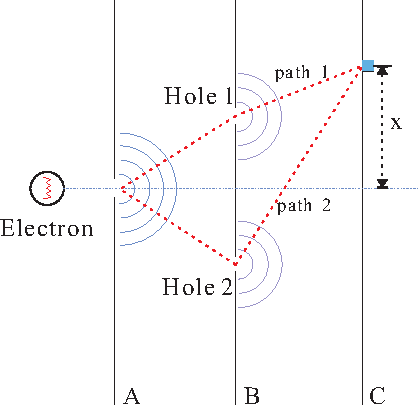
\includegraphics[width=6cm]{fig4.pdf}
  \caption{实验装置$A$处射出的电子前进到屏$C$处的探测器, 其间插入一个带有两个孔的屏$B$. 对于到达的每一个电子, 探测器记录下一个计数; 当探测器距离屏幕中心为$x$时, 测量电子到达的比例, 并以$x$进行标定, 如图\ref{Experiment solution}所示.}\label{pic-electron}
\end{figure}
如果探测器足够灵敏, 则会发现, 到达$x$的电流不是连续的, 而是一个个电子相继到达的. 若电子源$S$的强度足够弱, 探测器将会记录下一个个的脉冲. 脉冲时间间隔内没有电子到达, 因为这个原因, 我们说电子是粒子. 如果将探测器分布在屏$C$上的各个位置, 并且电子源$S$足够微弱, 那么一次只有一个探测器响应, 过间隔时间后另一个探测器才响应. 如此不断地连续下去. 探测器绝对不会出现半个响应或者同时多个响应. 也就是说, 要么一次一个电子的完整响应, 要么什么也没有. 换句话说, 探测器记录了电子从源$S$到$x$的经历.

\indent我们需要做的是对于不同位置$x$的探测器, 测量每秒钟脉冲的平均个数, 最后得到电子从$S$到$x$相对概率$P$作为$x$的函数. 概率$P$作为$x$函数的图像是一条复杂的曲线, 定性的画在下图, 它有极大值极小值, 在中心的附近一些区域几乎没有电子到达, 我们需要处理的物理问题就是找到这条曲线的规律.

\indent由于电子是粒子, 我们必须做出如下假定
\begin{enumerate}[I]
  \item 从$S$到达$x$的电子必须经过孔$1$或者$2$
  \item 到达$x$的概率应该是两部分之和, 也就是说通过孔$1$的概率$P_1$加上通过孔$2$的概率$P_2$.
  \item\label{Prob} 存在复数$\phi_1,\phi_2$使得
\begin{equation*}
  \begin{split}
     P & =|\phi|^2 \\
     \phi & =\phi_1+\phi_2 \\
     P_1 & =|\phi_1|^2,P_2=|\phi_2|^2
  \end{split}
\end{equation*}
\end{enumerate}
我们可以用实验来检验这是否正确. 每一组分的概率是容易测量的.只需要分别遮住不同孔就能得到单个孔对应的电子概率分布.如图\ref{Experiment solution}所示.

\indent根据图中的结果, 蓝色曲线完全与两单孔对应的两条曲线叠加之和不同, 说明$P\neq P_1+P_2$.
\begin{figure}[H]
  \centering
  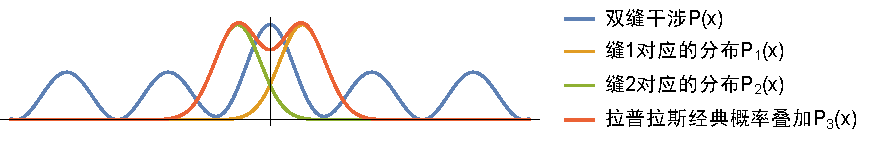
\includegraphics[width=14cm]{fig6.pdf}
  \caption{实验结果. 电子到达$x$的概率是相对探测器位置$x$画出的. 图\ref{pic-electron}的实验结果画在蓝色线中; 若仅仅只有孔$1$开启, 则电子仅仅能通过孔$1$,  其结果是绿色线所代表; 若仅仅孔$2$开启, 则是黄色线所代表的的结果. 如果我们设想每个电子恰好通过这个空或那个孔, 则当两孔都开启时, 预期得到的曲线应该是绿色线+黄色线=红色线. 这与实际所得的蓝色线大不相同.}\label{Experiment solution}
\end{figure}
\subsubsection{概率幅}
两孔都开启时, 电子到达$x$的概率并不是单独开启孔$1$的概率与单独开启孔$2$的概率之和.
\indent实际上, 复杂曲线$P(x)$是我们熟悉的电子通过两个孔后干涉叠加的分布强度曲线. 在波动力学里, 描述波是用复变函数$\phi(x)$描述的, 而$|\phi(x)|^2$正好描述了这个强度分布曲线$P(x)$, 而$\phi(x)$叫做电子到达$x$的概率幅. 这样我们就能用数学来描述$P(x)$的规律. 并且$\phi(x)$是两个孔对应$\phi_1(x),\phi_2(x)$之和.
\begin{figure}[H]
  \centering
  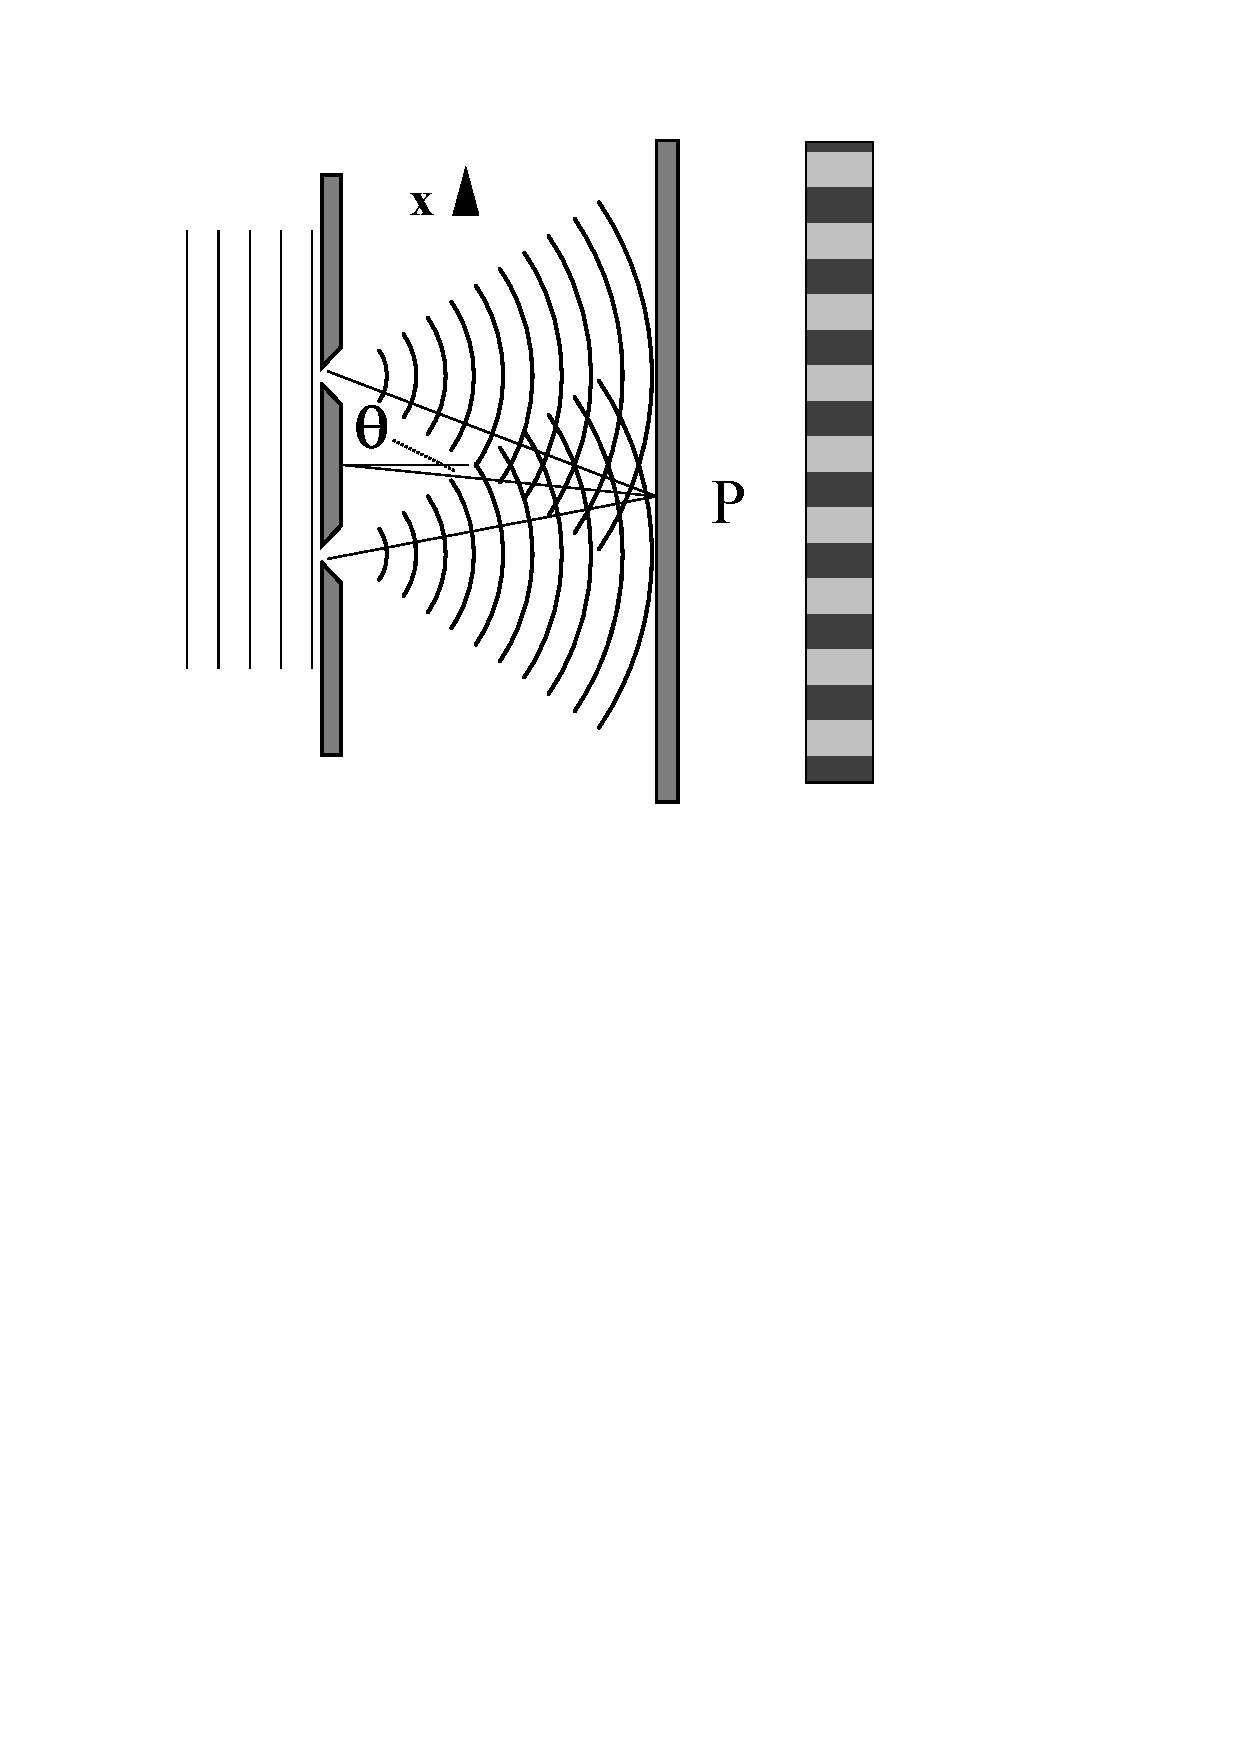
\includegraphics[width=6cm]{fig5.pdf}
  \caption{相干干涉叠加出的电子分布曲线有极大值也有极小值, 在一些点发自两个不同孔的电子相干相消, 在另一些点上发自不同孔的两个电子相干相长, 由此产生了电子分布曲线$I(x)$的条纹}\label{double slit 2}
\end{figure}
这样我们就能得到\ref{Prob}的推断.以后我们会介绍如何计算$\phi_1,\phi_2$. 总之, 我们能计算出到达$x$处探测器的波强度, 并且把这个强度解释为粒子到达$x$处的概率.
\subsubsection{测量问题}
值得注意的是, 这里我们描述电子的运动使用了波动力学里描述波用的复变函数$\phi(x)$. 这意味着我们应该抛弃经典力学里粒子与波的概念. 在量子力学里同时使用波的概念和粒子的概念并不产生矛盾.

\indent为了更详细地讨论这一点, 首先考虑观测结果是干涉条纹的情况. 新的概率叠加规律意味着$P_1+P_2=P$是不正确的. 这就导致了一个结论: 当两个孔开启时, 粒子通过这个孔或那个孔的说法是不对的. 因为如果粒子通过这个孔或那个孔, 我们可以根据通过的孔将粒子分为不相干的两类, 并且到达$x$的次数$P$一定是粒子经过孔$1$和孔$2$次数之和

\indent这与我们经典的理解完全不一样, 为了理解这点, 历史上曾经有人思考过电子也许在一条复杂的轨道上运动, 先通过孔$1$再以某种复杂的方式通过孔$2$; 或许电子以某种方式散开, 部分地通过两个孔, 导致最终的干涉结果; 或许由于遮住孔$2$有可能影响孔$1$附近的电子运动, 从而电子穿过孔$1$的概率没有正确的被确定, 人们曾经试图用许多这种经典力学模型去解释这个结果. 当我们使用光子时, 可以使干涉路径$1$和$2$在空间上相距几个厘米, 因此两个交叉轨道几乎肯定是独立的. 下面的实验可以证明, 实际情况比开始所设想的具有更深远的意义.
\paragraph*{观测的后果}\quad\\
\indent之前的逻辑推导得到的结果$P\neq P_1+P_2$. 这个结果可以说明根据电子通过孔$1$或者孔$2$来分析电子的运动是不正确的. 然而可以设计一个实验来验证这个结论, 在孔后面放一个光源, 就可以观看电子通过哪一个孔(如图\ref{Choose Experiment}). 由于电子散射光, 因此如果光在孔$1$后面被散射, 我们立马可以判定电子通过的是孔$1$; 若光在孔$2$后面被散射, 我们立马可以判定电子通过的是孔$2$.
\begin{figure}[H]
  \centering
  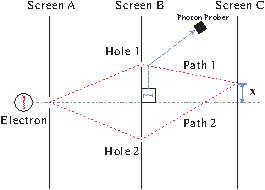
\includegraphics[width=10cm]{fig7.pdf}
  \caption{实验\ref{pic-electron}的一个修正. 我们在屏$B$后面放一个光源$L$, 并寻找通过孔$1$或者孔$2$的电子散射的光. 用一个很强的光源, 确实可以发现每个电子通过这个或那个孔. 但现在到达$x$的概率不再是由图\ref{Experiment solution}中的蓝线给出而是由图\ref{Experiment solution}中的红线给出.}\label{Choose Experiment}
\end{figure}
这个实验结果表示, 电子确实通过的孔$1$或者孔$2$. 对于每一个到达屏幕$C$的电子, 光要么在孔$1$后面被散射, 要么在孔$2$后面被散射,并且绝不会在两处同时被散射. (更精细的实验可以得到电子都是以一个完整电荷$e$出现的, 绝不会出现它的部分电荷.)

\indent这似乎引起了一个荒谬的问题. 假设将两个实验联合起来查看电子通过了哪个孔, 并同时测量电子到达$x$的概率, 然后对于每一个到达$x$的电子, 我们可以从实验上来说明电子是否通过了孔$1$或者孔$2$. 首先我们知道$P_1$由图\ref{Experiment solution}中的橙色曲线给出, 因为我们若选择到达$x$的电子只是通过孔$1$的电子, 则我们得到的正是橙色曲线$P_1$(孔$2$是否遮住均可得到这个结果, 因此可以说明孔$2$是否开启对孔$1$附近电子运动毫无影响). 如果选取孔$2$出散射光的电子, 我们得到的则是绿色曲线$P_2$. 现在每个电子要么出现在孔$1$要么出现在孔$2$, 并且可以将它分成不相干的两类. 因此如果我们把这两类放在一起, 一定得到的是红色曲线$P=P_1+P_2$, 实验确实如此. 然而该分布没有出现蓝色干涉曲线!

\indent这里发生的变化实际上是当我们观察电子通过哪个孔时, 就能得到结果$P=P_1+P_2$, 当我们观察时, 就得到不同的结果$P=|\phi_1+\phi_2|^2\neq P_1+P_2$.

\indent实际上正是我们观察了电子才改变了它到达$x$的概率. 为了观察电子, 我们是用了光, 而光与电子的碰撞会改变电子的运动, 或者更确切的说, 改变了电子到达$x$的概率.

\indent另一方面, 我们是否能使用较弱的光源来降低光对电子的影响呢? 事实上一个很弱甚至可以忽视的干扰对分布肯定不会产生从蓝色到红色曲线的有限小的改变. 但弱的光并不意味着弱的干扰. 光以能量$h\nu$或者动量$h/\lambda$的量子形式出, 减弱光意味着使用较少的光子. 因此我们会漏看一些电子. 但是当我们确实看见一个电子的时候, 就意味着一个完整的光子被散射, 并且这个电子获得大约为$h/\lambda$的有限动量.

\indent漏看的那些电子是根据干涉定律图\ref{Experiment solution}中蓝色曲线分布的, 而我们真正看到的是散射一个光子并到达$x$的那些电子, 这些电子的概率分布是图\ref{Experiment solution}中的红色曲线. 因此在这种情况下, 总的分布是蓝色曲线和红色曲线的加权平均. 在强的光线下, 几乎所有的电子都散射光, 分布近似红色曲线, 在弱的光线下, 散射极少, 它更相似于蓝色曲线.

\indent我们仍然可以认为, 既然光携带的动量是$h/\lambda$, 那么我们采用波长足够长的光就可以减弱影响效果. 但这是有限度的, 如果使用波长太长的光, 我们将不能区分电子到底从哪个孔后面被散射. 因为波长为$\lambda$的光源用于空间定位时, 其精度不超过$\lambda$的数量级.

\indent因此我们看到, 为测定电子通过哪个孔而设计的任何物理实验, 一定会产生强的干扰, 足以使分布从蓝色曲线变到红色曲线. 海森堡第一个注意到这些, 并在他的不确定性原理中作了陈述: 当时崭新的力学自洽性对所能进行的实验精度有一个限制. 在我们的情形中, 这个原理可以得出: 设计一种装置来测定电子通过什么样的孔, 并且足够精细, 使得电子的偏转不足以破坏干涉图形的企图一定不会成功. 量子力学自洽性要求这必须是一个普遍性的陈述. 对于不确定性原理, 从未发现过任何例外情况. 在后面的章节里, 我们会进一步讨论不确定性原理, 量子力学的不确定性是一种本质上的不确定性, 而不是实验所导致的.


\subsection{量子力学基础概念}
\subsubsection{量子态}
我们考虑一个微观量子系统, 它由具有一些物理特征(例如质量、电荷、角动量等)的粒子组成, 这些粒子之间按照力学规律去运动, 我们把每一种符合运动规律的状态叫做一个量子态. 按照经典力学的做法, 我们如果确定了这个力学系统的坐标$q$和动量$p$, 这个力学系统就确定下来了, 因为我们可以通过求解哈密顿正则方程去得到任何时刻的力学状态. 然而之前章节论证了, 对于一个量子系统, 存在不确定性, 我们无法的到这个力学系统所有的信息. 测量能力的局限性限制了一个量子态可以具有数据的数量. 这样就导致了量子系统的状态不能用某一个时刻的全部坐标与动量去确定, 而必须用比较少的数据, 或者一些具有概率性的数据来确定.
\begin{definition}[量子态的符号]
  在量子力学里, 一般使用符号$|\psi\rangle$表示一个量子态$\psi$, 其中$\psi$是量子态的记号. 在不同的系统里, 根据不同的情况可以采用不同的量子数去标记量子态. 例如$|\xi_1\xi_2\dots \xi_s\rangle$, 这里$\xi_1,\xi_2,\dots,\xi_s$是$s$个独立不同的量子数, 有些地方也用记号$|\psi_{\xi_1,\xi_2,\dots,\xi_s}\rangle$.
\end{definition}
\begin{example}
  坐标为$x$的电子的量子态用符号$|x\rangle$表示, 动量为$p$的电子用$|p\rangle$表示.
\end{example}
\indent在前面的干涉实验\ref{pic-electron}里, 我们讨论了干涉测量问题. 为了简化问题, 我们这里暂不考虑电子, 现在我们考虑一个单光子干涉的实验问题
\begin{figure}[H]
  \centering
  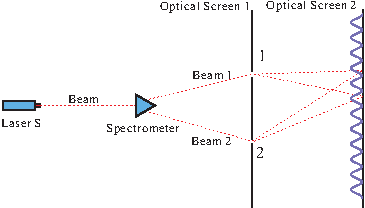
\includegraphics[width=10cm]{fig8.pdf}
  \caption{单光子干涉实验: 激光器发射一束激光通过分光器分为两束, 束流$1$通过孔$1$, 束流$2$通过孔$2$, 然后在光屏$2$上发生干涉. 若减弱激光器$S$, 以至于一束激光在足够长的时间内只射出一个光子, 该光子通过分光器后处于束流$1$的状态称作$|1\rangle$,处于 束流$2$的状态称作状态$|2\rangle$}\label{Single photon interference}
\end{figure}
\indent我们把通过孔$1$的状态标记为$|1\rangle$, 通过孔$2$的状态标记为$|2\rangle$. 如果我们减弱激光器功率, 一直到一束激光在足够长的时间内只有一个光子射出, 很自然我们会问到: 单个光子通过分光器后会走哪条路径? 这个问题看起来很怪异, 但实际上却指向了量子力学的核心. 若我们认为光子通过分光器后走孔$1$或者孔$2$对应的路径, 类似前面电子测量问题的分析, 孔$1$和孔$2$是独立的, 这就不可避免的让我们又回到了拉普拉斯概率性叠加$P=P_1+P_2$. 由前面的分析, 这点与我们所需要的量子力学并不符合.

\indent为了解决这个问题, 我们必须把光子描述成部分同时地进入由入射光分裂而成的两个组分$(|1\rangle,|2\rangle)$中的每一个. 这样我们可以说光子处于一个量子态, 这个量子态是分别由两个组分对应的状态(量子态)叠加而成. 用光学的语言来说就是, 每一个组分对应的量子态$|i\rangle$与普通波动力学中的波函数$\psi_i$相联系. 每一个波函数可以描述一个组分的光子, 而总的波函数是由各个组分的波函数$\psi_i$叠加而成, 因此量子态$|\cdot\rangle$可以像波函数一样线性叠加.

\begin{hypothesis}[量子态的线性叠加原理]\label{Superposition hypothesis}
  在量子力学中量子态满足线性叠加原理
\begin{equation*}
  |\psi\rangle=\sum_{n}c_n|\psi_n\rangle
\end{equation*}
其中$c_n\in\mathbb{C}$.
\end{hypothesis}
我们暂不考虑为什么量子力学是定义在复数域$\mathbb{C}$上的, 该后续章节会解释. 量子态$|\psi_n\rangle$满足线性叠加性, 这意味着$|\psi_n\rangle$在数域$\mathbb{C}$上构成了线性空间$E$. 我们把这个量子态$|\psi_n\rangle$构成的线性空间叫做态空间$E$, 态空间$E$的元素叫做态$|\psi_n\rangle$.
\begin{theorem}
  量子系统所有线性无关的量子态$|\psi_n\rangle,(n=1,2,\dots)$构成一个$\mathbb{C}$上的线性空间$E$, 量子力学里习惯叫做态空间. 这个系统任何时刻的量子态都处于态空间中, 并可以由不同量子态叠加得到
\end{theorem}
\begin{proof}
  根据量子态线性叠加的假设\ref{Superposition hypothesis}我们可以得到
\begin{equation*}
  \begin{split}
     c_1|\phi\rangle+c_2|\phi\rangle&=(c_1+c_2)|\phi\rangle \\
     c|\phi_1\rangle+c|\phi_2\rangle&=c(|\phi_1\rangle+|\phi_2\rangle)
  \end{split}
\end{equation*}
若$c_1+c_2=0$, 则有$|\phi\rangle+(-|\phi\rangle)=0$

\indent按照我们之前单光子实验的描述, 量子态的叠加态必须同时处于多个线性无关的组分中. 这意味着
\begin{equation*}
  \begin{split}
     |\phi_1\rangle+|\phi_2\rangle&=|\phi_2\rangle+|\phi_1\rangle\\
     (|\phi_1\rangle+|\phi_2\rangle)+|\phi_3\rangle&=|\phi_1\rangle+(|\phi_2\rangle+|\phi_3\rangle)
  \end{split}
\end{equation*}
这样就证明了量子态构成一个线性空间, 有些地方把量子态矢量简称为态矢量.
\end{proof}
\subsubsection{左矢量}
当我们建立起一个矢量集合之后, 我们总是能够通过矢量集合到数域$\mathbf{F}$之间的映射定义一个新的矢量集合, 我们叫做对偶矢量. 在物理系统里面最简单的到数域$\mathbf{F}$(量子力学里$\mathbf{F}=\mathbb{C}$)是量子态之间的内积
\begin{definition}[量子态的内积]
  在态空间$E$中的两个态矢量$|\varphi\rangle$与$|\psi\rangle$的内积定义为:
\begin{equation*}
  \langle\varphi|\psi\rangle=\phi
\end{equation*}
其中$\phi\in\mathbb{C}$, 这里$\langle\varphi|$称为左矢量, $|\psi\rangle$称为右矢量, $\phi$为复数.
\end{definition}
在\ref{Hilbert Space}章介绍了对偶空间的概念, 这里我们定义了量子态内积为$\langle\varphi|\phi\rangle\in\mathbb{C}$, 所以左矢量$\langle\phi|$是一个线性映射$L:|\phi\rangle\longmapsto\mathbb{C}$. 而根据\ref{Hilbert Space}章对偶空间的概念, 这意味着所有的左矢量也构成一个线性空间$E'$.
\begin{theorem}[态空间的对偶空间---左矢空间]
  对于一个给定的量子系统, 量子态的内积诱导出左矢空间$E'$, 左矢空间$E'$是右矢空间$E$的对偶空间, 其中两个态矢量的正交定义为:
\begin{equation*}
  \langle\varphi|\psi\rangle=0
\end{equation*}
\end{theorem}
\begin{proof}
\indent在第\ref{Hilbert Space}章的对偶空间里, 我们已经证明过. 这里我们从物理的角度说明一下.

\indent假定有一个数$\phi$, 它是右矢量$|\psi\rangle$的函数. 也就是对于每一个右矢量$|\psi\rangle$都有一个数$\psi$与之对应. 我们假定这个函数数是线性的, 意思是对应于$|\psi\rangle+|\psi'\rangle$的数是对应于$\psi\rangle$的数与对应于$|\psi\rangle$的数之和, 而对应于$c|\psi\rangle$的数等于$c$乘以对应于$|\psi\rangle$的数.($c\in\mathbb{C}$).因此我们可以把数$\phi$看成矢量$|\psi\rangle$与某个新的矢量的标量积, 每一个右矢量$|\psi\rangle$的线性函数都有一个这类新的矢量与之对应. 这个新的矢量就叫做左矢量. 我们假定对于线性函数$\phi$, $|\psi\rangle$对应的左矢量为$\langle\varphi|$. 它们之间的线性条件可以写成:
\begin{equation}\label{leftvec add 1}
  \begin{split}
     \langle\varphi|(|\psi\rangle+|\psi'\rangle)&=\langle\varphi|\psi\rangle+\langle\varphi|\psi'\rangle \\
     \langle\varphi|(c|\psi\rangle)&=c\langle\varphi|\psi\rangle
  \end{split}
\end{equation}
其中$c\in\mathbb{C}$.
\end{proof}

\begin{property}[左矢量的几个性质]\quad
\begin{enumerate}[(1)]
  \item 如果左矢量与任意右矢量的内积都完全确定下来, 那么左矢量就完全确定下来了. 特别是, 如果对所有的$|\psi\rangle$都有$\langle\varphi|\psi\rangle=0$, 则$\langle\varphi|=0$
  \item\label{leftvec add 2} 两个左矢量之和$\langle\varphi|+\langle\varphi'|$定义为它与任意右矢量的内积等于$\langle\varphi|$和$\langle\varphi'|$分别与$|\psi\rangle$的内积之和
\begin{equation}
  (\langle\varphi|+\langle\varphi'|)|\psi\rangle=\langle\varphi|\psi\rangle+\langle\varphi'|\psi\rangle
\end{equation}
  \item\label{scale leftvec} 左矢量$\langle\varphi|$与$\mathbb{C}$中的标量$c$的乘积为$(c\langle\varphi|)|\psi\rangle=c\langle\varphi|\psi\rangle$
\end{enumerate}
\end{property}
方程\eqref{leftvec add 1}和性质\ref{leftvec add 2}与性质\ref{scale leftvec}表明, 左右矢量的乘法都满足分配律, 它们与复数域的标量$c$的乘积满足结合律.

\indent这里所引入的左矢量是与右矢量完全不同的矢量, 到目前为止, 它们之间没有任何联系, 只是在左右矢量之间存在标量积(内积). 现在我们给定一个左右矢量之间一个新的假设, 以建立起左右矢量之间的一一对应关系.
\begin{hypothesis}
  我们假定对应于$|\psi\rangle+|\psi'\rangle$的左矢量等于对应于$|\psi\rangle$的左矢量和对应于$|\psi‘\rangle$的左矢量之和, 而对应于$c|\psi\rangle$的左矢量等于$c^*$乘对应于$|\psi\rangle$的左矢量. 其中$c^*$是$c$的复共轭.
\end{hypothesis}
建立起这种对应关系后, 我们可以用相同的记号来表示与右矢量$|\psi\rangle$对应的左矢量$\langle\psi|$. 左右矢量之间的这种一一对应关系建立起来之后, 量子动力学系统在任意时刻$t$的任何状态既可以用右矢量$|\psi(t)\rangle$表示也可以用左矢量$\langle\psi(t)|$来表示. 事实上整个理论在左右矢量是对称的.

\begin{theorem}[左右矢量与量子态的对应关系]
  对应于两个独立量子态的叠加态$c_1\phi_1+c_2\phi_2$, 对应的右矢量为$c_1|\phi_1\rangle+c_2|\phi_2\rangle$, 左矢量为$c_1^*\langle\phi_1|+c_2^*\langle\phi_2|$.
\begin{equation*}
  \begin{split}
     &\text{量子态}\phi\longleftrightarrow\text{右矢量}|\phi\rangle\longleftrightarrow\text{左矢量}\langle\phi|\\
     &\text{量子态}c_1\phi_1+c_2\phi_2\longleftrightarrow\text{右矢量}c_1|\phi_1\rangle+c_2|\phi_2\rangle\longleftrightarrow\text{左矢量}c_1^*\langle\phi_1|+c_2^*\langle\phi_2|\\
  \end{split}
\end{equation*}
\end{theorem}
这样我们可以使用一个统一的符号来用左右矢量表示量子态:
\begin{equation*}
  \begin{split}
     \text{量子态}c\phi & \longmapsto|c\phi\rangle=c|\phi\rangle \\
     \text{量子态}c\phi & \longmapsto\langle c\phi|=c^*\langle\phi|
  \end{split}
\end{equation*}
给定两个量子态$\varphi$和$\phi$, 我们有它们的内积$\langle\varphi|c\psi\rangle=c\langle\varphi|\psi\rangle$与$\langle c\psi|\varphi\rangle=c^*\langle\psi|\varphi\rangle$.这使得我们进行进一步的假设:
\begin{hypothesis}[态矢量内积复共轭]
给定量子态$\varphi$与$\psi$, 我们假定它们的内积$\langle\varphi|\psi\rangle$与$\langle\psi|\varphi\rangle$之间满足复共轭
\begin{equation*}
  \langle\varphi|\psi\rangle=\langle\psi|\varphi\rangle^*
\end{equation*}
\end{hypothesis}
\indent在这个假设下, 令$\langle\varphi|=\langle\psi|$, 很显然$\langle\psi|\psi\rangle$是实数. 这样我们进一步假定\footnote{这是为了用内积去定义范数而做的假设.}除$|\psi\rangle=0$外
\begin{equation}\label{braket proper}
  \langle\psi|\psi\rangle>0
\end{equation}

\indent在之前的干涉实验里, 概率叠加满足概率幅的线性叠加原理$|\phi|^2=|\psi_1+\psi_2|^2$, 并且概率幅的模方满足正定性$|\psi_i|^2\geq 0$与三角不等式$|\phi_1+\phi_2|<|\phi_1|+|\phi_2|$. 根据量子态和右矢量之间的对应性, 再考虑到线性空间内积和范数的联系. 我们可以定义量子态的范数.
\begin{theorem}[范数]\label{ket norm}
  在态空间$E$中, 任意量子态$\psi$对应的右矢量$|\psi\rangle$的范数$\||\psi\rangle\|$为
\begin{equation*}
  \||\psi\rangle\|=\sqrt{\langle\psi|\psi\rangle}
\end{equation*}
\end{theorem}
\begin{proof}
  \indent首先正定性显然满足$\||\psi\rangle\|=\sqrt{\langle\psi|\psi\rangle}>0$

\indent接下来证明三角不等式$\||\varphi\rangle\|+\||\psi\rangle\|>\||\varphi+\psi\rangle\|$
\begin{equation*}
  \begin{split}
     \||\varphi\rangle+|\psi\rangle\|^2 & =(\langle\varphi|+\langle\psi|)(|\varphi\rangle+|\psi\rangle) \\
       & =\langle\varphi|\varphi\rangle+\langle\varphi|\psi\rangle+\langle\psi|\varphi\rangle+\langle\psi|\psi\rangle \\
       & =\langle\varphi|\varphi\rangle+2Re(\langle\varphi|\psi\rangle)+\langle\psi|\psi\rangle\\
       & <\langle\varphi|\varphi\rangle+2|\langle\varphi|\psi\rangle|+\langle\psi|\psi\rangle\\
       & <\langle\varphi|\varphi\rangle+2\||\varphi\rangle\|\|\psi\rangle\|+\langle\psi|\psi\rangle\\
       & =(\||\varphi\rangle\|+\||\psi\rangle\|)^2
  \end{split}
\end{equation*}
\end{proof}
\begin{definition}\label{ket normalization}
  给定一个右矢量$|\psi\rangle$, 我们可以构成一个归一的右矢量$|\tilde{\psi}\rangle$, 记为:
\begin{equation*}
  |\tilde{\psi}\rangle=\frac{|\psi\rangle}{\langle\psi|\psi\rangle}
\end{equation*}
它有下列性质:
\begin{equation*}
  \langle\tilde{\psi}|\tilde{\psi}\rangle=1
\end{equation*}
\end{definition}
由于归一化, 在物理学中我们认为$|\psi\rangle$和$c|\psi\rangle$在$c\neq0$时表示同一个物理态. 换句话说, 态空间中只有方向是有意义的.

\indent根据正定性假设\ref{braket proper}和归一化条件\ref{ket normalization}, 很自然会做一个假设:归一化态矢量$|\psi\rangle$的自身内积$\langle\psi|\psi\rangle$对应物理测量\footnote{测量问题会在算符谱理论中进行解释}得到的\textbf{总概率}$1$.

\indent实验\ref{Single photon interference}可以看出, 物理系统总是要求一个量子系统态矢量的集合$E$是完备的. 从物理的要求上来说, 态空间$E$必须是$Hilbert$空间$\mathcal{H}$, 其中状态矢量是$Hilbert$空间$\mathcal{H}$的一个元素. 所有的量子力学演化过程都发生在$Hilbert$空间$\mathcal{H}$里, 这使得我们可以利用$Hilbert$空间$\mathcal{H}$来描述量子力学.用数学的语言来说:
\begin{theorem}[完备性]\label{Quantum Parseval}
  若$\{|\psi_n\rangle\}\subset\mathcal{H}$是一组完备正交基. 则对于任意$|\varphi\rangle\subset\mathcal{H}$.
\begin{equation*}
  \|\varphi\|^2=\sum_{n}|\langle\varphi|\psi_n\rangle|^2
\end{equation*}
\end{theorem}
该定理实质上就是Parseval关系. 证明过程在\ref{Parseval formula}. 在之前的章节里, 介绍了Hilbert空间里可以通过Schmidt正交化$\mathcal{H}^n$得到一组完备正交归一的基向量${|\psi_n\rangle}$. $\mathcal{H}$中任意向量都可以用这组完备正交归一的基展开.
\begin{equation*}
  |\psi\rangle=\sum_{k}c_k|\psi_n\rangle
\end{equation*}
其中$c_k=\langle\psi_k|\psi\rangle$. 如果$\mathcal{H}$包含一组正交归一基, 则叫$\mathcal{H}$为可分的Hilbert空间.
\section{算符理论}
\subsection{线性算符}
在之前的章节里我们建立起了一套描述量子力学所需要的数学, 很自然地就会想到, 态空间中两个不同的右矢量之间有何联系. 实际上我们希望建立起两个不同量子态$\psi\mapsto\varphi$之间的联系, 而这两个量子态之间的联系对应的物理实际意义正是这章我们要讨论的核心内容. 在实际物理实验中, 可以制备许多相同的量子态(纯态$\{|\phi_1\rangle,|\phi_2\rangle,\dots,|\phi_n\rangle\}$), 而在这些相同的量子态测量相同的力学量(例如角动量、动量、能量等)会得到不同的取值结果(返回值). 在经典力学里, $n$个相同的状态分别测量相同力学量得到的n个结果必定一样, 这意味着量子力学里的力学量与经典力学里的力学量并不一样. 量子力学与经典力学之间的矛盾暗含了量子力学中的力学量应该对应着一个测量值的分布. 线性算符正好满足这个性质, 线性算符具有谱, 正好对应着量子力学的测量值分布. 线性算符的性质直接与实际物理相互对应.
\subsubsection{线性算符}
\begin{definition}[线性算符]
  $\mathcal{H}$中的线性算符$\hat{A}$是指映射$A:\mathcal{H}\longmapsto\mathcal{H}$, $\hat{A}$满足线性关系
\begin{equation*}
  \hat{A}(\alpha|\varphi\rangle+\beta|\psi\rangle)=\alpha \hat{A}|\varphi\rangle+\beta \hat{A}|\psi\rangle
\end{equation*}
其中$|\varphi\rangle, |\psi\rangle\in\mathcal{H},\alpha,\beta\in\mathbb{C}$.
\end{definition}
实际上我们只需要算符$\hat{A}$定义在定义域$\mathcal{D}(\hat{A})\subset\mathcal{H}$, 其中定义域$\mathcal{D}(\hat{A})$在$\mathcal{H}$中稠密:
\begin{equation*}
  A:\mathcal{D}(\hat{A})\longmapsto\mathcal{H}
\end{equation*}
下面是一些$\mathcal{H}$上线性算符的例子.
\begin{example}\quad
  \begin{enumerate}[1]
    \item 恒等映射
\begin{equation*}
  \mathbf{1}:|\psi\rangle\longmapsto|\psi\rangle
\end{equation*}
    \item 坐标算符
\begin{equation*}
  \hat{x}_j:|\psi\rangle\longmapsto \hat{x}_j|\psi\rangle
\end{equation*}
    \item 动量算符
\begin{equation*}
  \hat{p}_j:|\psi\rangle\longmapsto \hat{p}_j|\psi\rangle
\end{equation*}
    \item 两个不同量子态$\psi\longmapsto\varphi=\hat{A}\psi$
\begin{equation*}
  \hat{A}:|\psi\rangle\longmapsto|\varphi\rangle=|\hat{A}\psi\rangle=\hat{A}|\psi\rangle
\end{equation*}
  \end{enumerate}
\end{example}
\indent我们是用右矢量$|\psi\rangle$去标记量子态$\psi$, 右矢量与量子态之间存在对应$\psi\longleftrightarrow|\psi\rangle$, 右矢量与左矢量之间又存在线性对偶$|\psi\rangle\stackrel{Dual}{\longmapsto}\langle\psi|$. 这就可以在量子态, 右矢量和左矢量之间建立起算符的对应.
\begin{equation*}
  \begin{split}
     \text{量子态:}\psi & \longmapsto\varphi=\hat{A}\psi \\
     \text{右矢量:}|\psi\rangle & \longmapsto|\varphi\rangle=|\hat{A}\psi\rangle=\hat{A}|\psi\rangle \\
     \text{左矢量:}\langle\psi| & \longmapsto\langle\varphi|=\langle\hat{A}\psi|
  \end{split}
\end{equation*}
两个不同线性算符的乘积也可以利用线性映射定义\\
\begin{minipage}[b]{0.75\linewidth}
\begin{definition}[线性算符的乘积]
    $\mathcal{H}$中两个线性算符$\hat{A},\hat{B}$的乘积定义为
\begin{equation*}
  (\hat{A}\hat{B})|\psi\rangle=\hat{A}|\hat{B}\psi\rangle=\hat{A}(\hat{B}|\psi\rangle)
\end{equation*}
其中$|\psi\rangle\in\mathcal{H}$.
\end{definition}
\end{minipage}
\begin{minipage}[b]{0.25\linewidth}
  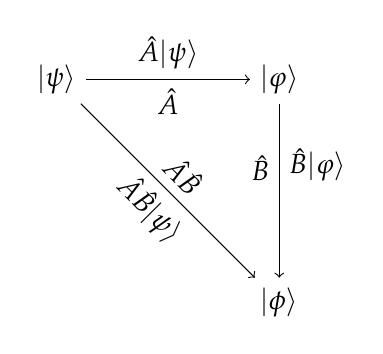
\begin{tikzpicture}
  \node (phi) at (315:2) {$|\phi\rangle$};
  \node (varphi) at (45:2) {$|\varphi\rangle$} edge [->] node[above left] {$\hat{B}$} node[above right] {$\hat{B}|\varphi\rangle$} (phi);
  \node (psi) at (135:2) {$|\psi\rangle$} edge [->] node[below,sloped] {$\hat{A}$} node[above,sloped] {$\hat{A}|\psi\rangle$} (varphi)
                                          edge [->] node[above,sloped] {$\hat{A}\hat{B}$} node[below,sloped] {$\hat{A}\hat{B}|\psi\rangle$} (phi);
\end{tikzpicture}
\end{minipage}

\indent在定理\ref{Quantum Parseval}里, 我们得到了量子力学完备性条件(Parseval公式). 这里可以进一步写成算符形式.
\begin{theorem}[完备性条件]\label{Quantum Completed condition}
  若$\{|\psi_n\rangle:|\psi_n\in\mathcal{H}\}$是态空间$\mathcal{H}$中的一组完备正交归一向量的集合, 则有完备性条件
\begin{equation*}
  \sum_{n}|\psi_n\rangle\langle\psi_n|=\mathbf{1}
\end{equation*}
其中$\mathbf{1}$是单位算符$\mathbf{1}_{n\times n}$.
\end{theorem}
\begin{proof}
  根据上一节的Parseval公式\ref{Quantum Parseval}有
\begin{equation*}
  \begin{split}
     \||\varphi\rangle\|^2&=\sum_{n}|\langle\varphi|\psi_n\rangle|^2 \\
       & =\sum_{n}\langle\varphi|\psi_n\rangle\langle\psi_n|\varphi\rangle \\
       & =\langle\varphi|\left(\sum_{n}|\psi_n\rangle\langle\psi_n|\right)|\varphi\rangle \\
       & =\langle\varphi|\varphi\rangle
  \end{split}
\end{equation*}
所以
\begin{equation*}
  \sum_{n}|\psi_n\rangle\langle\psi_n|=\mathbf{1}
\end{equation*}
\end{proof}
\subsubsection{有界算符和逆算符}
\begin{definition}[有界算符]
  算符$\hat{A}$是$\mathcal{H}$上的有界算符定义为
\begin{equation}\label{Bound operator}
  \|\hat{A}\|:=\sup_{\{|\psi\rangle\in\mathcal{H}|\|\psi\|=1\}}\|\hat{A}|\psi\rangle\|<\infty
\end{equation}
\end{definition}
\indent事实上, 表达式\ref{Bound operator}定义了一个范数, 它使$\mathcal{H}$上有界算符的空间$B(\mathcal{H})$成为一个Banach空间. 我们将会看到在一些方面有界算符比无界算符要容易处理的多. 然而, 由于量子力学中一些最重要的算符是无界的, 我们需要研究它们的性质.

\indent通常我们可以证明在定义域$\mathcal{D}$上稠密的算符$A$一致有界. 下面这个引理表示, 在这种情况下, $A$可以推广到有界算符.
\begin{lemma}
  如果算符$A$在定义域$\mathcal{D}\subset\mathcal{H}$上稠密, 对于$\psi$满足$\|\hat{A}|\psi\rangle\|\leq C\||\psi\rangle\|$(C与$\psi$无关), 则它可以扩展到$\mathcal{H}$上的有界算符, 满足相同的界:
\begin{equation*}
  \|\hat{A}|\psi\rangle\|\leq C\||\psi\rangle\|,\quad|\psi\rangle\in\mathcal{H}
\end{equation*}
\end{lemma}
\begin{proof}
  对于任意$|\psi_n\rangle\in\mathcal{H}$, 有序列$\{|\psi_n\rangle\}\subset \mathcal{D}$使得当$n\to\infty$时$|\psi_n\rangle\to|\psi\rangle$($\mathcal{D}$的稠密性). 则关系
\begin{equation*}
  \|\hat{A}|\psi_n\rangle-\hat{A}|\psi_m\rangle\|\leq C\|\psi_n\rangle-|\psi_m\rangle\|
\end{equation*}
表明了$\{A|\psi_n\rangle\}$是一个Cauchy序列, 所以对于一些$|\varphi\rangle\in\mathcal{H}$, $\hat{A}|\psi_n\rangle\to|\varphi\rangle$, 我们令$\hat{A}|\psi\rangle:=|\varphi\rangle$.

\indent因为$\|\hat{A}|\psi\rangle\|=\lim\|\hat{A}|\psi_n\rangle\|\leq C\lim\|\psi_n\rangle\|=C\||\psi\rangle\|$, 这使$\hat{A}$扩展到$\mathcal{H}$上的有界算符, 有相同的界$C$.
\end{proof}
对于特定重要的一类算符, 反过来说也成立:定义在$\mathcal{H}$上的算符必须是有界的. 这样的一类算符是闭算符.
\begin{definition}[有界算符]\label{Closed operator def}
  $\mathcal{H}$上有算符$\hat{A}$.若对于任意的序列${|\psi_j\rangle}_{j=1}^{\infty}\subset\mathcal{D(\hat{A})}$, 其中当$j\to\infty$时,$|\psi_j\rangle\to|\psi\rangle, A|\psi_j\rangle\to|\varphi\rangle$, 可以的得到$|\psi\rangle\in\mathcal{D}(\hat{A})$以及$\hat{A}|\psi\rangle=|\varphi\rangle$, 则$\hat{A}$被叫做闭算符. 换句话说, $\hat{A}$的图$\{(|\psi\rangle,\hat{A}|\psi\rangle):|\psi\rangle\in\mathcal{D}(\hat{A})\}\subset\mathcal{H}\times\mathcal{H}$是封闭的.
\end{definition}
另一类算符是对称算符.
\begin{definition}[对称算符]\label{Symmetric operator}
  若满足下列条件时, 算符$\hat{A}$是对称算符
\begin{equation*}
  \langle\varphi|\hat{A}\psi\rangle=\langle\hat{A}\varphi|\psi\rangle
\end{equation*}
其中$\varphi,\psi\in\mathcal{D}(\hat{A})$.
\end{definition}
量子力学里最重要的算符是对称算符, 特别是自伴算符, 这将会在下节介绍.
\begin{theorem}\label{Bounded operator theorem}
  定义在全体$\mathcal{H}$上的闭算子或对称算子是有界的.
\end{theorem}
\begin{proof}
  对于闭算符, 这是闭图象定理. 对于对称算符, 则是Hellinger-Toeplitz定理.
\end{proof}
\begin{definition}[逆算符]
  给定Hilbert空间$\mathcal{H}$上算符$\hat{A}$, 满足下列条件的算符$\hat{B}$称为算符$\hat{A}$的逆算符. 如果$\mathcal{D}(\hat{B})=\mathcal{R}(\hat{A}), \mathcal{D}(\hat{A})=\mathcal{R}(\hat{B})$,
\begin{equation*}
  \hat{B}\hat{A}=\mathbf{1}|_{\mathcal{R}(\hat{A})}\quad\hat{A}\hat{B}=\mathbf{1}_{\mathcal{R}(B)}
\end{equation*}
这里
\begin{equation*}
  \mathcal{R}(\hat{A}):=\{\hat{A}|\psi\rangle:|\psi\rangle\in \mathcal{D}(\hat{A})\}
\end{equation*}
表示$\hat{A}$的值域
\end{definition}
\indent从该定义可以得出, 算符$\hat{A}$最多只能有一个逆. 算符$\hat{A}$的逆记作$\hat{A}^{-1}$. 换句话说, 找到$\hat{A}$的逆等价于求解方程$\hat{A}|\psi\rangle=|\varphi\rangle$, 其中$|\varphi\rangle\in\mathcal{R}(A)$.

\indent判断算符$\hat{A}$有逆的一个准则是:$\hat{A}$是一一映射. 也就是说, $\hat{A}|\psi\rangle=0\Longrightarrow|\psi\rangle=0$, 或者等价于它是平凡核或者零空间:
\begin{equation}\label{operator inverse 1}
  \mathrm{Ker}\,(\hat{A}):=\left\{|\psi\rangle\in\mathcal{D}(\hat{A}):\hat{A}|\psi\rangle=0\right\}=\{0\}
\end{equation}
如果$\hat{A}$具有有界逆, 则称算符$\hat{A}$是可逆的. 由于有界算符是定义在$\mathcal{H}$上的, 所以除了一一映射之外, 可逆算符$\hat{A}$还必须有:
\begin{equation}\label{operator inverse 2}
  \mathcal{R}(\hat{A})=\mathcal{H}
\end{equation}
\indent条件\ref{operator inverse 1}和\ref{operator inverse 2}确保了$A^{-1}$的存在, 并且$A^{-1}$定义在$\mathcal{H}$上. 事实上, 在一些重要的情况下, 它们足以确保$\hat{A}$确实是可逆的(即$A^-1$是有界的) , 即:
\begin{enumerate}
  \item 如果$\hat{A}$是闭算符, 根据定义\ref{Closed operator def}, $A^{-1}$也是, 因此根据定理\ref{Bounded operator theorem}, $A^{-1}$是有界的.
  \item 如果$\hat{A}$是对称算符, 那么根据定理\ref{Bounded operator theorem}$A^{-1}$也是对称算符.
\end{enumerate}
\begin{theorem}\label{A+B inverse}
  $\hat{A}$是可逆算符, $\hat{B}$是有界算符, 并且满足$\|\hat{B}\hat{A}^{-1}\|<1$. 那么定义在$\mathcal{D}(\hat{A}+\hat{B})=\mathcal{D}(\hat{A})$算符$\hat{A}+\hat{B}$是可逆的
\end{theorem}
这个关系式遵循关系式$\hat{A}+\hat{B}=(\mathbf{1}+\hat{B}\hat{A}^{-1})\hat{A}$
\subsubsection{练习题}
\begin{problem}[可逆算符的乘积]
  证明:若算符$\hat{A}$和$\hat{B}$都是可逆的, 并且$\hat{B}$是闭算符, 则算符$\hat{B}\hat{A}$定义在$\mathcal{D}(\hat{B}\hat{A})=\mathcal{D}(\hat{A})$并且是可逆的, 逆算符满足$(\hat{B}\hat{A})^{-1}=\hat{A}^{-1}\hat{B}^{-1}$
\end{problem}
\begin{problem}[Neumann级数]\label{Neumann series}
  证明满足$\|\hat{A}\|<1$的有界算符$\hat{A}$, 级数$\sum_{n=0}^{\infty}(-\hat{A})^n$是绝对收敛的, 并且它的逆算符是$1+\hat{A}$.
\begin{equation*}
  (1+\hat{A})^{-1}=\sum_{n=0}^{\infty}(-\hat{A})^n
\end{equation*}
\end{problem}
\subsection{自伴算符(厄米算符)和投影算符}
\subsubsection{自伴算符}
在量子力学里自伴算符扮演着核心角色. 本节专门讨论这类算符以及更广泛的对称算符. 所有的算符都假定定义在稠密的定义域$\mathcal{D}(\hat{A})$上
\begin{definition}[自伴算符]\label{Self-adjoint def 1}
  Hilbert空间$\mathcal{H}$上有线性算符$\hat{A}$, 若$\hat{A}$是对称的且$\mathcal{R}(\hat{A}+i\mathbf{1})=\mathcal{H}$, 则$\hat{A}$是自伴算符.
\end{definition}
值得注意, 条件$\mathcal{R}(\hat{A}+i\mathbf{1})=\mathcal{H}$等价于方程
\begin{equation*}
  (\hat{A}+i\mathbf{1})\psi=f
\end{equation*}
\indent对于所有的$f\in\mathcal{H}$有解.上述定义与通常用的定义不同, 但实质上是等价的. 这样定义自伴算符隐藏了我们真正需要的自伴算符性质, 并避免了与我们无关的冗长证明.

\indent与上述定义等价的一个常用定义是利用伴算符来定义的.
\begin{definition}[伴算符]\label{Self-adjoint def 2}
  Hilbert空间$\mathcal{H}$上的算符$\hat{A}^{\dag}$满足下列关系叫做伴算符:
\begin{equation}\label{Adjoint operator}
  \langle\hat{A}\varphi|\psi\rangle=\langle\varphi|\hat{A}^{\dag}\psi\rangle
\end{equation}
对于所有的$|\psi\rangle\in\mathcal{D}(\hat{A})$以及对于定义域
\begin{equation*}
  \mathcal{D}(\hat{A}^{\dag}):=\{\varphi\in\mathcal{H}:\text{对于某些与$|\psi\rangle$无关的常数}C_{\varphi}, |\langle\varphi|\hat{A}\psi\rangle|\leq C_{|\varphi\rangle}\||\psi\rangle\|,\forall|\psi\rangle\in\mathcal{D}(\hat{A})\}
\end{equation*}
中的$|\varphi\rangle$都成立
\end{definition}
\indent之前我们定义了对称算符\ref{Symmetric operator}, 这里我们引入一种特殊的对称算符,叫做自伴算符.
\begin{definition}
  若$\hat{A}^{\dag}=\hat{A}$, 则算符$\hat{A}$是自伴算符
\end{definition}
\indent根据自伴算符的定义, 每一个自伴算符都是对称算符. 事实上确实如此, 算符$\hat{A}$是自伴算符当且仅当它是对称的且$\mathcal{D}(\hat{A})=\mathcal{D}(\hat{A}^{\dag})$. 但是不是所有的对称算符都是自伴算符, 每一个自伴算符也不能唯一的扩展到更大的自伴定义域, 后面的章节里会接触这类问题.
\indent接下来我们会说明有界对称算符是自伴算符. 为了说明这一点, 我们先引入一个引理.
\begin{lemma}\label{sym operator lemma}
  设$\hat{A}$是对称算符. 若存在一些$z$($Im z>0$)有$\mathcal{R}(\hat{A}-z\mathbf{1})=\mathcal{H}$, 则对于$Im z>0$的每一个$z$都成立.同样的, 对于$Im z<0$也有相同的结论. 进一步说, 若$\hat{A}$是自伴算符, 则对于每个$Im z\neq0$的$z$, $\hat{A}-z\mathbf{1}$是可逆的, 并且满足估计
\begin{equation}\label{sym estimate}
  \|(\hat{A}-z\mathbf{1})^{-1}\|\leq\frac{1}{|Im z|}
\end{equation}
\end{lemma}
\begin{proof}
  记$z=\lambda+i\mu\quad\lambda,\mu\in R$.由于$\hat{A}$是对称算符, 我们有
\begin{equation}\label{symmetric operator proof}
  \begin{split}
     \|(\hat{A}-z\mathbf{1})|\psi\rangle\|^2 & =\langle(\hat{A}-z\mathbf{1})\psi|(\hat{A}-z\mathbf{1})\psi\rangle \\
       & =\langle(\hat{A}-(\lambda+i\mu)\mathbf{1})\psi|(\hat{A}-(\lambda+i\mu)\mathbf{1})\psi\rangle \\
       & =\langle(\hat{A}-\lambda\mathbf{1})\psi|(\hat{A}-\lambda\mathbf{1})\psi\rangle-i\mu\langle(\hat{A}-\lambda\mathbf{1})\psi|\psi\rangle+i\mu\langle\psi|(\hat{A}-\lambda\mathbf{1})\psi\rangle+\mu^2\langle\psi|\psi\rangle\\
       & =\|(\hat{A}-\lambda\mathbf{1})|\psi\rangle\|^2+\||\mu\psi\rangle\|^2\geq|\mu|^2\||\psi\rangle\|^2
  \end{split}
\end{equation}
因此, 若$Im z>0$(或者$Imz<0$), 则$\mathrm{Ker}\,(A-z)={0}$. 若$\mathcal{R}(\hat{A}-z\mathbf{1})=\mathcal{H}$, 则$(\hat{A}-z)^{-1}$定义在全体$\mathcal{H}$. 进一步说, 式子\eqref{symmetric operator proof}意味着$(\hat{A}-z\mathbf{1})^{-1}$是有界的, 界由\eqref{sym estimate}确定(如果定义$|\varphi\rangle:=(\hat{A}-z\mathbf{1})|\psi\rangle$), 所以特别是$(\hat{A}-z\mathbf{1})$是可逆的. 那么根据定理\ref{A+B inverse}, 对于$|z'-z|<\|(\hat{A}-z\mathbf{1})^{-1}\|^{-1}$, $\hat{A}-z'\mathbf{1}=(\hat{A}-z\mathbf{1})+(z\mathbf{1}-z'\mathbf{1})$是可逆的. 因此如果$|z'-z|<|Im z|$,$A-z'\mathbf{1}$是可逆的, 所以我们可以拓展$\hat{A}-z\mathbf{1}$的可逆性到全体$Im z'>0$(或者$Imz'<0$)上. 若$\hat{A}$是自伴的, 则$\mathcal{R}(\hat{A}\pm i=\mathcal{H})$, 因此$\hat{A}-z\mathbf{1}$是可逆的且对于$z\in\mathbb{C}$满足\ref{sym estimate}.
\end{proof}
这个引理表示了若$\hat{A}$是自伴的, 则对于任意$\alpha\neq0$的实数$\alpha,\beta$, $\alpha\hat{A}+\beta$也是自伴的以及:
\begin{equation*}
  \text{$\hat{A}$是自伴算符}\Rightarrow\text{对于$\forall Im z\neq0$},\; (\hat{A}-z\mathbf{1})|\psi\rangle=|\phi\rangle\text{有唯一的解}
\end{equation*}
下面这个定理显示了对于有界算符, 自伴性很容易检验.
\begin{theorem}
  若$\hat{A}$是有界对称算符, 则$\hat{A}$是自伴算符.
\end{theorem}
\begin{proof}
  根据引理\ref{sym operator lemma}, 足以表明$\mathcal{R}(\hat{A}+i\lambda\mathbf{1})$提供的$|\lambda|$足够大. 这等价于对于$|\phi\rangle\in\mathcal{H}$和这个$\lambda$求解方程
\begin{equation*}
  (\hat{A}+i\lambda\mathbf{1})|\psi\rangle=|\phi\rangle
\end{equation*}
两边除以$i\lambda$得到
\begin{equation*}
  (\mathbf{1}+\hat{K}(\lambda))|\psi\rangle=|\varphi\rangle
\end{equation*}
其中$\hat{K}(\lambda)=(i\lambda)^{-1}\hat{A}, |\varphi\rangle=(i\lambda)^{-1}|\phi\rangle$. 令$|\lambda|>\|V\|$. 则$\|\hat{K}(\lambda)\|=\frac{1}{\lambda}\|\hat{A}\|<1$, 我们也推断出$(\mathbf{1}+\hat{K}(\lambda))$是可逆的(习题\ref{Neumann series}).
\end{proof}
\subsubsection{投影算符}
\begin{definition}
  设$\mathcal{H}$是Hilbert空间. 如果有界算符$\hat{P}\in\mathcal{H}$满足下面条件, 则叫做投影算符
\begin{equation*}
  \hat{P}^2=\hat{P}
\end{equation*}
\end{definition}
这个关系意味着$\|\hat{P}\|\leq\|\hat{P}\|^2$, 所以$\|\hat{P}\|\geq1$规定了$\hat{P}\neq
0$. 我们有
\begin{equation}\label{projection operator}
  |\phi\rangle\in\mathcal{R}(\hat{P})\Longleftrightarrow\hat{P}|\phi\rangle=|\phi\rangle\quad\text{和}\quad|\phi\rangle\in(\mathcal{R}(\hat{P}))^{\perp}\Longleftrightarrow\hat{P}^{\dag}|\phi\rangle=0
\end{equation}
确实, 如果$|\phi\rangle\in\mathcal{R}(\hat{P})$, 则存在$|psi\rangle\in\mathcal{H}$使得$|\phi\rangle=\hat{P}|\psi\rangle$, 所以$\hat{P}|\phi\rangle=\hat{P}^2|\psi\rangle=\hat{P}|\psi\rangle=|\phi\rangle$.
\begin{example}[几个投影算符的例子]
  \begin{enumerate}{(1)}
    \item 令$\mathcal{H}=L^2(\mathbb{R}^n)$, $E$是$\mathbb{R}^n$的子集. 则
    \begin{equation*}
      \chi_{x\in E}:f(x)\mapsto\chi_{E}(x)f(x)
    \end{equation*}
    其中
    \begin{equation*}
      \chi_{E}(x):=\left\{
                     \begin{array}{ll}
                       1\quad & \hbox{$x\in E$;} \\
                       0\quad & \hbox{$x\notin E$.}
                     \end{array}
                   \right.
    \end{equation*}
    是投影
    \item\label{Projection Hilbert} $\mathcal{H}$是任意的Hilbert空间, 且$\varphi,\psi\in\mathcal{H}$满足$\langle\varphi,\psi\rangle=1$. 则
        \begin{equation*}
          \phi\mapsto\langle\varphi,\phi\rangle\psi
        \end{equation*}
        是一个投影
    \item 如\ref{Projection Hilbert}里一样, 但现在有一个正交归一的基组\footnote{$\langle\psi_i,\psi_j\rangle=\delta_{ij}$}$\{\psi_{i}\}_{i=1}^N$. 则有
        \begin{equation*}
          \psi\mapsto\sum_{i}^{N}\langle\psi_i,\psi\rangle\psi_i
        \end{equation*}
        是一个投影
    \item 如上例, 只是此时Hilbert空间是$\mathcal{H}$是态空间, 同样的设有一组正交归一的基组$\{|\psi_k\}$. 则
        \begin{equation}\label{Projection ket}
          |\psi\rangle\mapsto\sum_{k}\langle\psi_k|\psi\rangle|\psi_k\rangle
        \end{equation}
        是一个投影.

        \indent由于$\langle\psi_k|\psi\rangle\in\mathbb{C}$, 式子\eqref{Projection ket}可以写成
        \begin{equation*}
          |\psi\rangle\mapsto\sum_{k}|\psi_k\rangle\langle\psi_k|\psi\rangle
        \end{equation*}
        \indent若将$|\psi_k\rangle\langle\psi_k|$看成算符映射
        \begin{equation*}
          |\psi_k\rangle\langle\psi_k|:|\psi\rangle\longmapsto|\psi_k\rangle
        \end{equation*}
        \indent这表明了算符$|\psi_k\rangle\langle\psi_k|$是一个投影算符$\hat{P}=|\psi_k\rangle\langle\psi_k|$
  \end{enumerate}
\end{example}
\begin{definition}
  \begin{enumerate}
    \item 如果投影算符$\hat{P}$有$\dim\mathcal{R}(\hat{P})=r$, 则称其秩$rank\;r<\infty$
    \item 如果投影算符$\hat{P}$是自伴的, 则被称为正交投影算符. 即$\hat{P}=\hat{P}^{\dag}$.
  \end{enumerate}
\end{definition}
若$\hat{P}$是正交投影算子, 则式子\eqref{projection operator}意味着
\begin{equation*}
  |\psi\rangle\perp\mathcal{R}(\hat{P})\Longleftrightarrow\hat{P}|\psi\rangle=0
\end{equation*}
即:$\mathrm{Ker}(\hat{P})=\mathcal{R}(\hat{P})^{\perp}$
上面的四个例子中除了第二个例子不是正交投影, 其余三个例子都是正交投影\footnote{特别应该注意$|\psi_k\rangle\langle\psi_k|$是正交投影算符}. 而第二个例子是正交的当且仅当$\varphi=\psi$
\subsubsection{练习题}
\begin{problem}
  证明方程\ref{Adjoint operator}定义了$D(\hat{A}^{\dag})$上唯一的线性算符
\end{problem}
\begin{problem}
  证明自伴算符两种定义\ref{Self-adjoint def 1}与\ref{Self-adjoint def 2}是等价的.

\indent\textbf{提示}:利用
\begin{lemma}
  若$\hat{A}$是有界对称算符, 则$\hat{A}$是自伴算符.
\end{lemma}
\end{problem}
\begin{problem}
  证明式子\eqref{projection operator}.
\end{problem}
\begin{problem}
  证明:
\begin{enumerate}
  \item 当且仅当$|\psi\rangle\perp\mathcal{R}(\hat{P})$时, $\hat{P}^{\dag}|\psi\rangle=0$
  \item $\mathcal{R}(\hat{P})$是闭的
  \item $\hat{P}^{\dag}$也是投影算符
\end{enumerate}
\end{problem}
\begin{problem}
  设$\hat{P}$是正交投影算符. 证明
  \begin{enumerate}
    \item $\|\hat{P}\|\leq1$, 所以若$\hat{P}\neq0$, 则$\|\hat{P}\|=1$;
    \item $1-\hat{P}$也是正交算符, 并且$\mathcal{R}(1-\hat{P})\perp\mathcal{R}(\hat{P}), \mathrm{Ker}\,(1-\hat{P})=\mathcal{R}(\hat{P})$;
    \item $\mathcal{H}=\mathcal{R}(\hat{P})\oplus \mathrm{Ker}\,\hat{P}$
  \end{enumerate}
\end{problem}
\subsection{谱理论}
迄今为止我们只在抽象的Hilbert空间中定义了算符, 而我们想要找到算符与实际物理对应的量是什么. 我们希望某些算符对应了某些物理量, 这些物理量正好是实验上可以观测的. 我们观测到的结果总是一个以某种概率分布出现的数值. 同时我们看到算符是具有谱结构的, 我们希望算符的谱能对应实际物理的结果. 这驱动我们去学习算符的一个重要特征------谱
\subsubsection{算符的谱}

\subsubsection{算符函数与谱映射定理}
\subsection{可观测力学量}
迄今为止我们已经基本建立起了Hilbert空间上右矢量、左矢量、线性算符. 很自然的会问到, 这样定义的数学对应的物理是什么. 在上一节里, 自伴算符满足$\hat{A}=\hat{A}^{\dag}$, 也就是$\langle\hat{A}\varphi|\psi\rangle=\langle\varphi|\hat{A}^{\dag}\psi\rangle=\langle\varphi|\hat{A}\psi\rangle$. 我们在上一章构建了右矢量的对偶, 也就是左矢量. 由于左矢量和右矢量之间存在一一映射, 左矢量空间实质上与右矢量空间同构. 我们所希望构建的一个新理论(量子力学)应该在左右矢量之间是对称的, 也就是左右矢量满足的运动方程实质上应该是一样的, 力学量在左右矢量之间应该是对称的. 这不得不使我们猜想, 量子力学里的力学量可能是自伴算符.
\begin{definition}
  具有可观测效应的物理量叫做力学量
\end{definition}
所谓可观测效应是指在实验测量过程中总是能够被观测到的量. 比如动量$p$, 角动量$J$, 自旋\footnote{粒子自旋是一个没有经典力学量对应的力学量, 但是我们可以通过观测粒子的磁矩得到自旋值}$s$. 所谓不可观测的物理量是指那些仅仅具有数学意义, 而无论设计多么巧妙的实验都无法观测的量\footnote{例如幺正幺模算符$\hat{U}$, 宇称算符$\hat{P}$, 时间反演算符$\hat{T}$等等, 都不可观测.}.
\begin{hypothesis}
  力学量是自伴算符, 用符号$\hat{A}$表示, 满足
\begin{equation*}
  \langle\hat{A}\psi|\psi\rangle=\langle\psi|\hat{A}^{\dag}\psi\rangle=\langle\psi|\hat{A}\psi\rangle
\end{equation*}
即$\hat{A}=A^{\dag}$.
\end{hypothesis}
由于这个假设, 我们通常在写力学量与态矢量乘积的时候并不区分力学量$\hat{A}$在左矢量上还是在右矢量上. 统一可以记作$\langle\psi|\hat{A}|\psi\rangle$, 力学量$\hat{A}$可以向后乘$\langle\psi|\overrightarrow{\hat{A}}|\psi\rangle$也可以向左乘$\langle\psi|\overleftarrow{\hat{A}}|\psi\rangle$.

\section{量子化}
\subsection{基本物理学量}
\subsection{表象变换与本征态}
\subsection{李乘法}
\subsection{基本量子化条件}
\subsection{不确定关系}
\section{量子动力学}
\subsection{薛定谔方程}
\subsubsection{能量本征方程}
\subsubsection{概率流守恒}
\subsubsection{一维well问题举例}
\subsection{单参数幺模群——时间演化算符}
\subsection{传播子与格林函数}
\subsection{动力学图像——薛定谔图像、海森堡图像、狄拉克图像}
\section{量子力学对称性}
\subsection{平移对称性与动量}
\subsection{转动对称性与角动量}
\subsection{李群李代数及其表示}
\subsection{角动量及其耦合}
\subsection{不可约张量算符}
\section{三维束缚态}
\subsection{渐进分析}
\subsection{无限深球well}
\subsection{有限深球well}
\subsection{三维谐振子}
\subsection{氢原子严格解}
\section{三维散射态}
\subsection{经典散射与微分截面}
\subsection{含时散射}
\subsection{$S-matrix$}
\subsection{Dyson公式}
\subsection{Born近似}
\section{多粒子量子系统}
\subsection{全同粒子与交换对称性}
\subsection{置换群与杨图、杨算子}
\subsection{二次量子化}
\subsection{电磁场正则量子化}
\subsection{Casmir效应}
\part{相对论量子力学}
\section{连续场基本方程}
\subsection{欧拉-拉格朗日方程}
\subsection{诺特原理与诺特流}
\subsection{克莱因-高登方程}
\subsection{克莱因-高登方程正则量子化}
\section{洛伦兹群}
\subsection{洛伦兹变换}
\subsection{Clifford代数的表示——$\gamma$矩阵}
\subsection{狄拉克方程}
\subsection{狄拉克方程正则量子化}
\subsection{洛伦兹群的分离对称性与电荷对称性——$\mathcal{CPT}$联合不变性}
\section{微扰理论}
\subsection{Gellman-Low公式与真空}
\subsection{Wick定理}
\subsection{Feynman图与费曼规则}
\subsubsection{$\phi^4$的费曼规则}
\subsubsection{QED的费曼规则}
\subsection{截面与$S$矩阵元}
\section{树图计算}
\subsection{$e^+e^-\rightarrow\mu^+\mu^-$}
\subsection{康普顿散射}
\subsection{库仑散射}
\section{圈图计算}
\subsection{顶角近似}
\subsection{辐射修正,正规化方案——PV方案}
\subsection{场强重整化}
\subsection{LSZ约化定理}
\subsection{光学定理}
\subsection{Ward-Takahashi恒等式}
\subsection{电荷重整化}
\part{规范理论}
\section{$U(1)$规范理论}
\section{$SU(n)$规范理论}
\subsection{规范理论的内禀空间与底流形}
\subsection{规范自由与纤维丛}
\subsection{规范固定与截面}
\subsection{Yang-Mills方程}
\subsection{Wilson圈}
\section{路径积分量子化}
\subsection{量子力学的路径积分}
\subsection{标量场的量子化}
\subsection{QED的量子化}
\subsection{旋量场的量子化}
\section{$Non-Abel$规范场量子化}
\subsection{Faddeev-Poppov路径积分量子化}
\subsection{鬼}
\subsection{BRST对称性}
\subsection{$Non-Abel$场的单圈修正}
\subsection{渐进自由}
\section{量子色动力学}
\subsection{夸克理论}
\subsection{胶子辐射}
\subsection{强子散射:轻子对}
\section{微扰理论}
\subsection{二维手征流}
\subsection{四维手征流}
\subsection{Goldstone定理}
\subsection{手征流反常}
\section{自发对称性破缺}
\subsection{Higgs机制}
\subsection{弱相互作用的Glashow-Weinberg-Salam理论}
\end{document} 